\chapter{Convolutional neural network evaluation} %%%%%%%%%%%%%%%%%%%%%%%%%%%%%%%%%%%%%%%%%%%%%%%%
\label{chap:results} %%%%%%%%%%%%%%%%%%%%%%%%%%%%%%%%%%%%%%%%%%%%%%%%%%%%%%%%%%%%%%%%%%%%%%%%%%%%%

\section{Performance} %%%%%%%%%%%%%%%%%%%%%%%%%%%%%%%%%%%%%%%%%%%%%%%%%%%%%%%%%%%%%%%%%%%%%%%%%%%%
\label{sec:results_eval} %%%%%%%%%%%%%%%%%%%%%%%%%%%%%%%%%%%%%%%%%%%%%%%%%%%%%%%%%%%%%%%%%%%%%%%%%

Here the performance of the CNN approach is presented and compared to that achieved by the
standard \chips methods outlined in Section.~\ref{sec:cnn_old} as well as other experiments. Again
it must be highlighted that the primary aim is the selection of an efficient and pure appeared CC
$\nu{e}$ sample for which the neutrino energy can be estimated well. Alongside this selection, the
secondary CC $\nu_{\mu}$ selection is also presented below for completeness.

Firstly, however, one key and hugely impactful advantage of the CNN approach must be highlighted.
Although the full time taken to train the CNNs of this work is approximately two days, once
trained the time required to calculate all network outputs (inference time) for a single event is
on the order of \unit{2}{\mathrm{ms}}. When combined with event seeding and map generation, the
total time taken to reconstruct and classify a raw event fully is roughly
\unit{0.2}{\mathrm{seconds}}.

Armed with this incredible speed, when split across multiple computing nodes, the time taken to
process an extensive Monte Carlo dataset containing millions of events becomes a matter of a few
hours. When compared to the multiple weeks typically required using standard methods, the
far-reaching implications for quick iteration of analyses becomes clear. By removing the
processing bottleneck, larger datasets can be used, and new analysis techniques can be implemented
without concern.

\subsection{Evaluation sample and preselection} %%%%%%%%%%%%%%%%%%%%%%%%%%%%%%%%%%%%%%%%%%%%%%%%%%
\label{sec:results_eval_sample} %%%%%%%%%%%%%%%%%%%%%%%%%%%%%%%%%%%%%%%%%%%%%%%%%%%%%%%%%%%%%%%%%%

A statistically independent sample of events is used to evaluate the combined performance of the
trained CNNs. The evaluation sample consists of 400000 beam and 350000 cosmic muon events,
produced in the same way as the training and validation events using the detector simulation and
event generation methods outlined in Section.~\ref{sec:chips_monte_carlo} with a \chipsfive
geometry. The beam events include the expected $\nu_{\mu}$, $\bar{\nu}_{\mu}$, $\nu_{e}$ and
$\bar{\nu}_{e}$ components of the beam as well as events generated to mimic the appeared(App)
$\nu_{e}$ component. In this work, only the neutrino mode (forward horn current) of NuMI beam
operation is considered for simplicity.

All evaluation events are weighted to match the expected spectrum in the \unit{5}{\mathrm{kton}}
\chipsfive detector, using the expected unoscillated flux, cross-sections, and oscillation
probabilities (including the MSW effect). Additional weighting also scales events to match data
taking in the NuMI beam for a year, corresponding to $6\times 10^{20}$ protons on target (POT).
Cosmic muon events are weighted according to the \unit{11.8}{\mathrm{kHz}} and
\unit{48}{\mathrm{m}} of overburden outlined in Section.~\ref{sec:chips_monte_carlo_cosmic}. For
simplicity, the neutrino and antineutrino components of the beam are also combined as they are
impossible to tell apart in practice. The final weighted spectrum of events is shown in
Fig.~\ref{fig:explore_osc_fluxes}. Furthermore, the evaluation sample contains the expected
combination of underlying neutrino interaction types, as shown in
Fig.~\ref{fig:explore_stacked_int_types}.

\begin{figure} % OSC FLUXES DIAGRAM %
    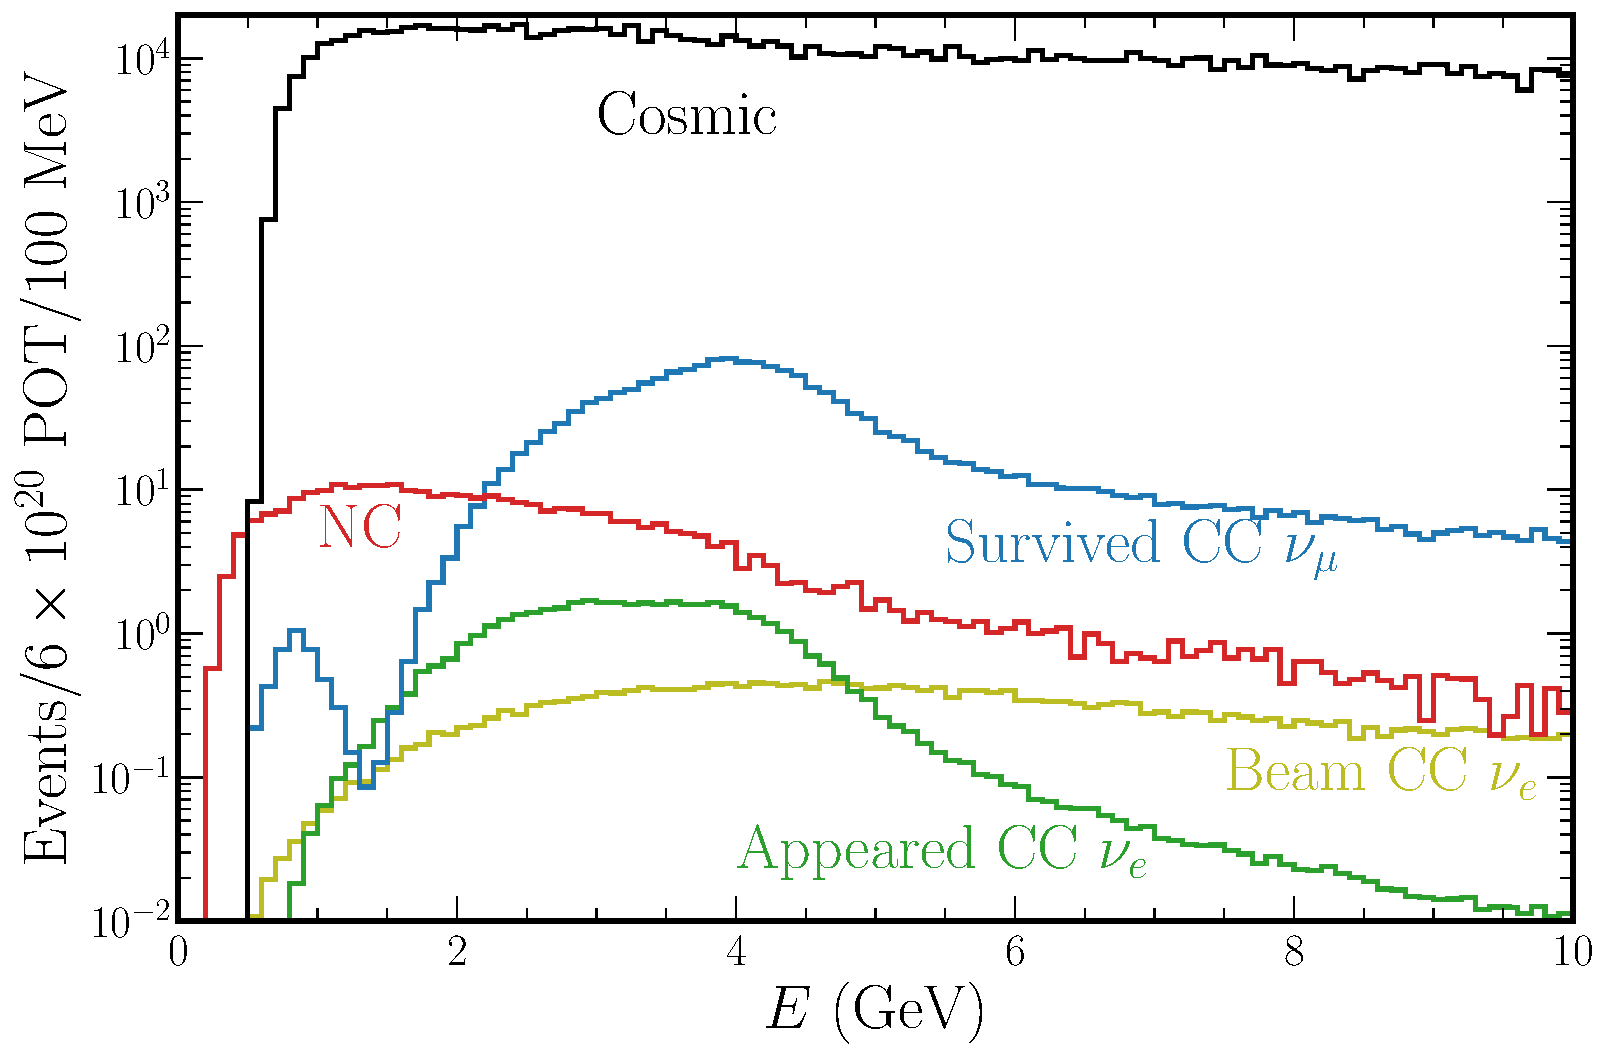
\includegraphics[width=0.7\textwidth]{diagrams/7-results/explore_osc_fluxes.pdf}
    \caption[Weighted spectrum of evaluation sample events]
    {Weighted spectrum of events contained within the evaluation sample. The weighting is designed
        to mimic the expected event spectrum of the \chipsfive detector. Beam events are weighted by
        combining the expected unoscillated flux with cross-sections and standard oscillation
        probabilities, while cosmic events are weighted using the expected cosmic rate and overburden.
        Shown in blue, green and olive are the surviving CC $\nu_{\mu}$, appearing CC $\nu_{e}$ and
        the intrinsic beam CC $\nu_{e}$ spectra respectively, binned in terms of their neutrino
        energy. Additionally, shown in red is the NC event spectra binned in terms of the energy of
        the hadronic component (excluding the outgoing neutrino energy) to represent more accurately
        the energy visible to the detector. Finally, shown in black is the cosmic muon event spectra
        binned in terms of the muon energy.}
    \label{fig:explore_osc_fluxes}
\end{figure}

\begin{figure} % STACK INT TYPES DIAGRAM %
    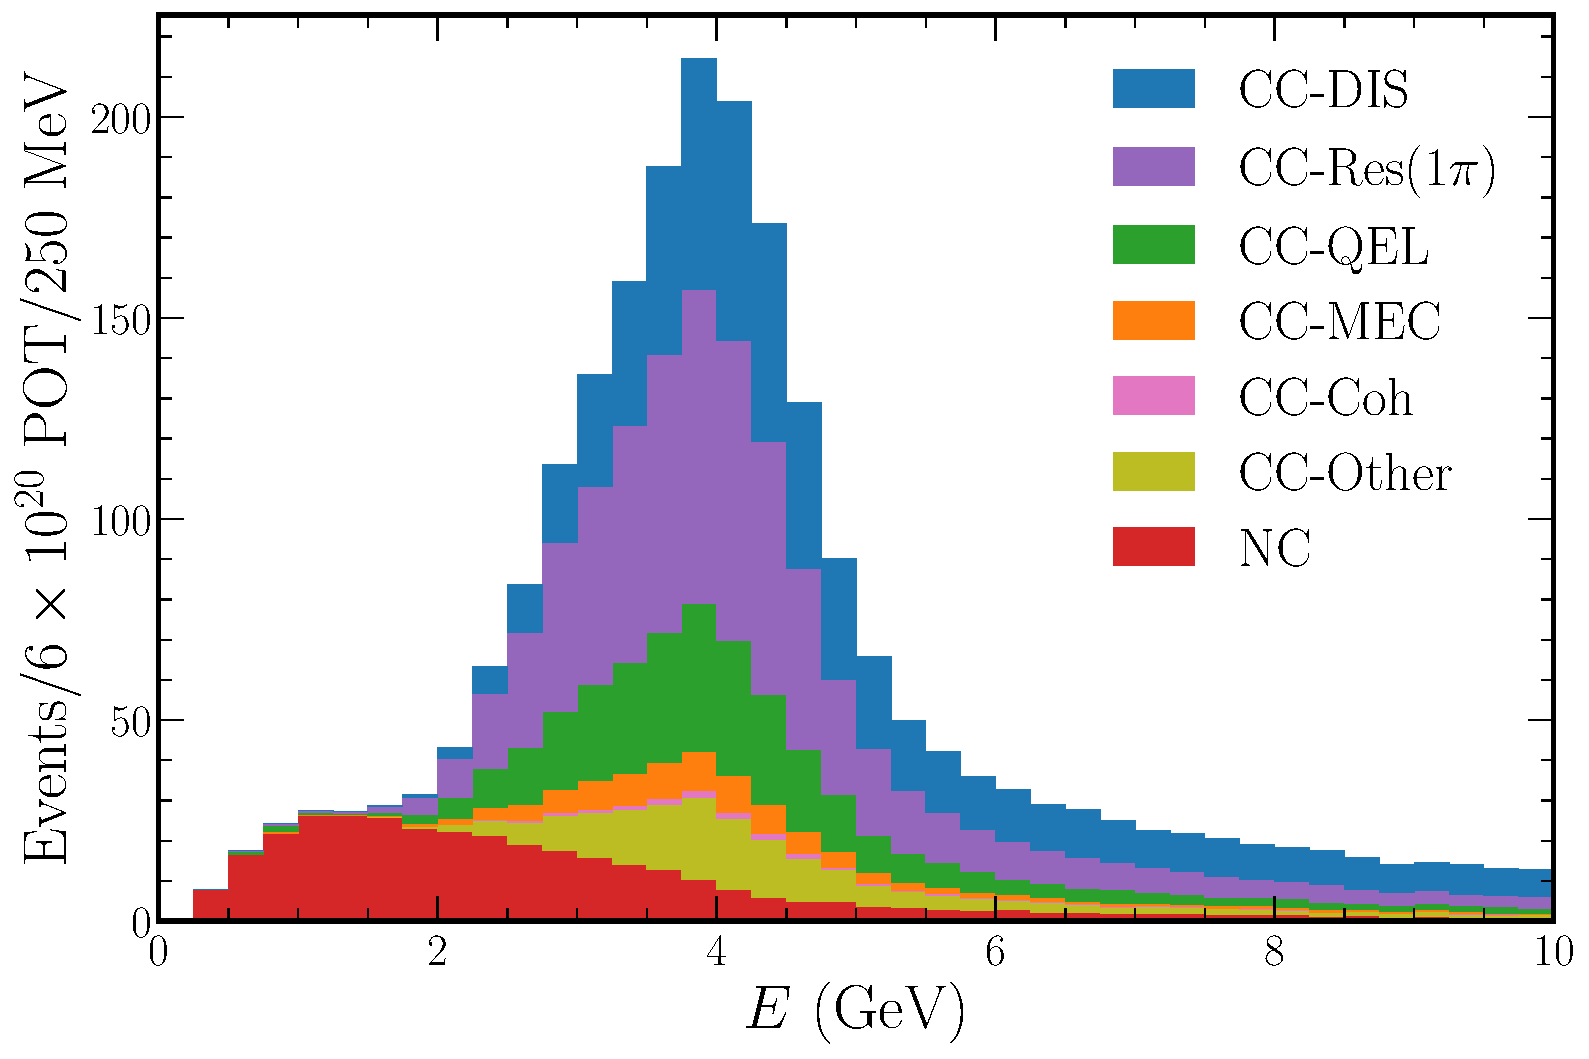
\includegraphics[width=0.7\textwidth]{diagrams/7-results/explore_stacked_int_types.pdf}
    \caption[Weighted spectrum of interaction types within the evaluation sample]
    {Weighted spectrum of $\nu_{\mu}$ and $\nu_{e}$ beam events contained within the evaluation
        sample separated by interaction type. CC events are binned in terms of neutrino energy while
        NC events are binned in terms of the hadronic component energy.}
    \label{fig:explore_stacked_int_types}
\end{figure}

Separate from the CNN driven work, a simple preselection is applied to all evaluation sample
events. Designed to reject cosmic and NC events while keeping the efficiency of CC beam events
high, the preselection consists of four simple cuts, shown in Fig.~\ref{fig:explore_simple_cuts}.
Firstly, the total number of collected photoelectrons (charge) across all PMTs in the event must
be greater than 250. Secondly, the maximum Hough transform space height must be greater than 250
photoelectrons. Thirdly, the leading seed $\cos(\theta)$ direction must be between $\pm$0.7.
Finally, the leading seed $\phi$ direction must be between $\pm$1.1 radians. The first two cuts
reject low energy events which are usually NC in nature, while the last two reject events whose
activity is not along the beamline, typically cosmic.

\begin{figure} % SIMPLE CUTS DIAGRAM %
    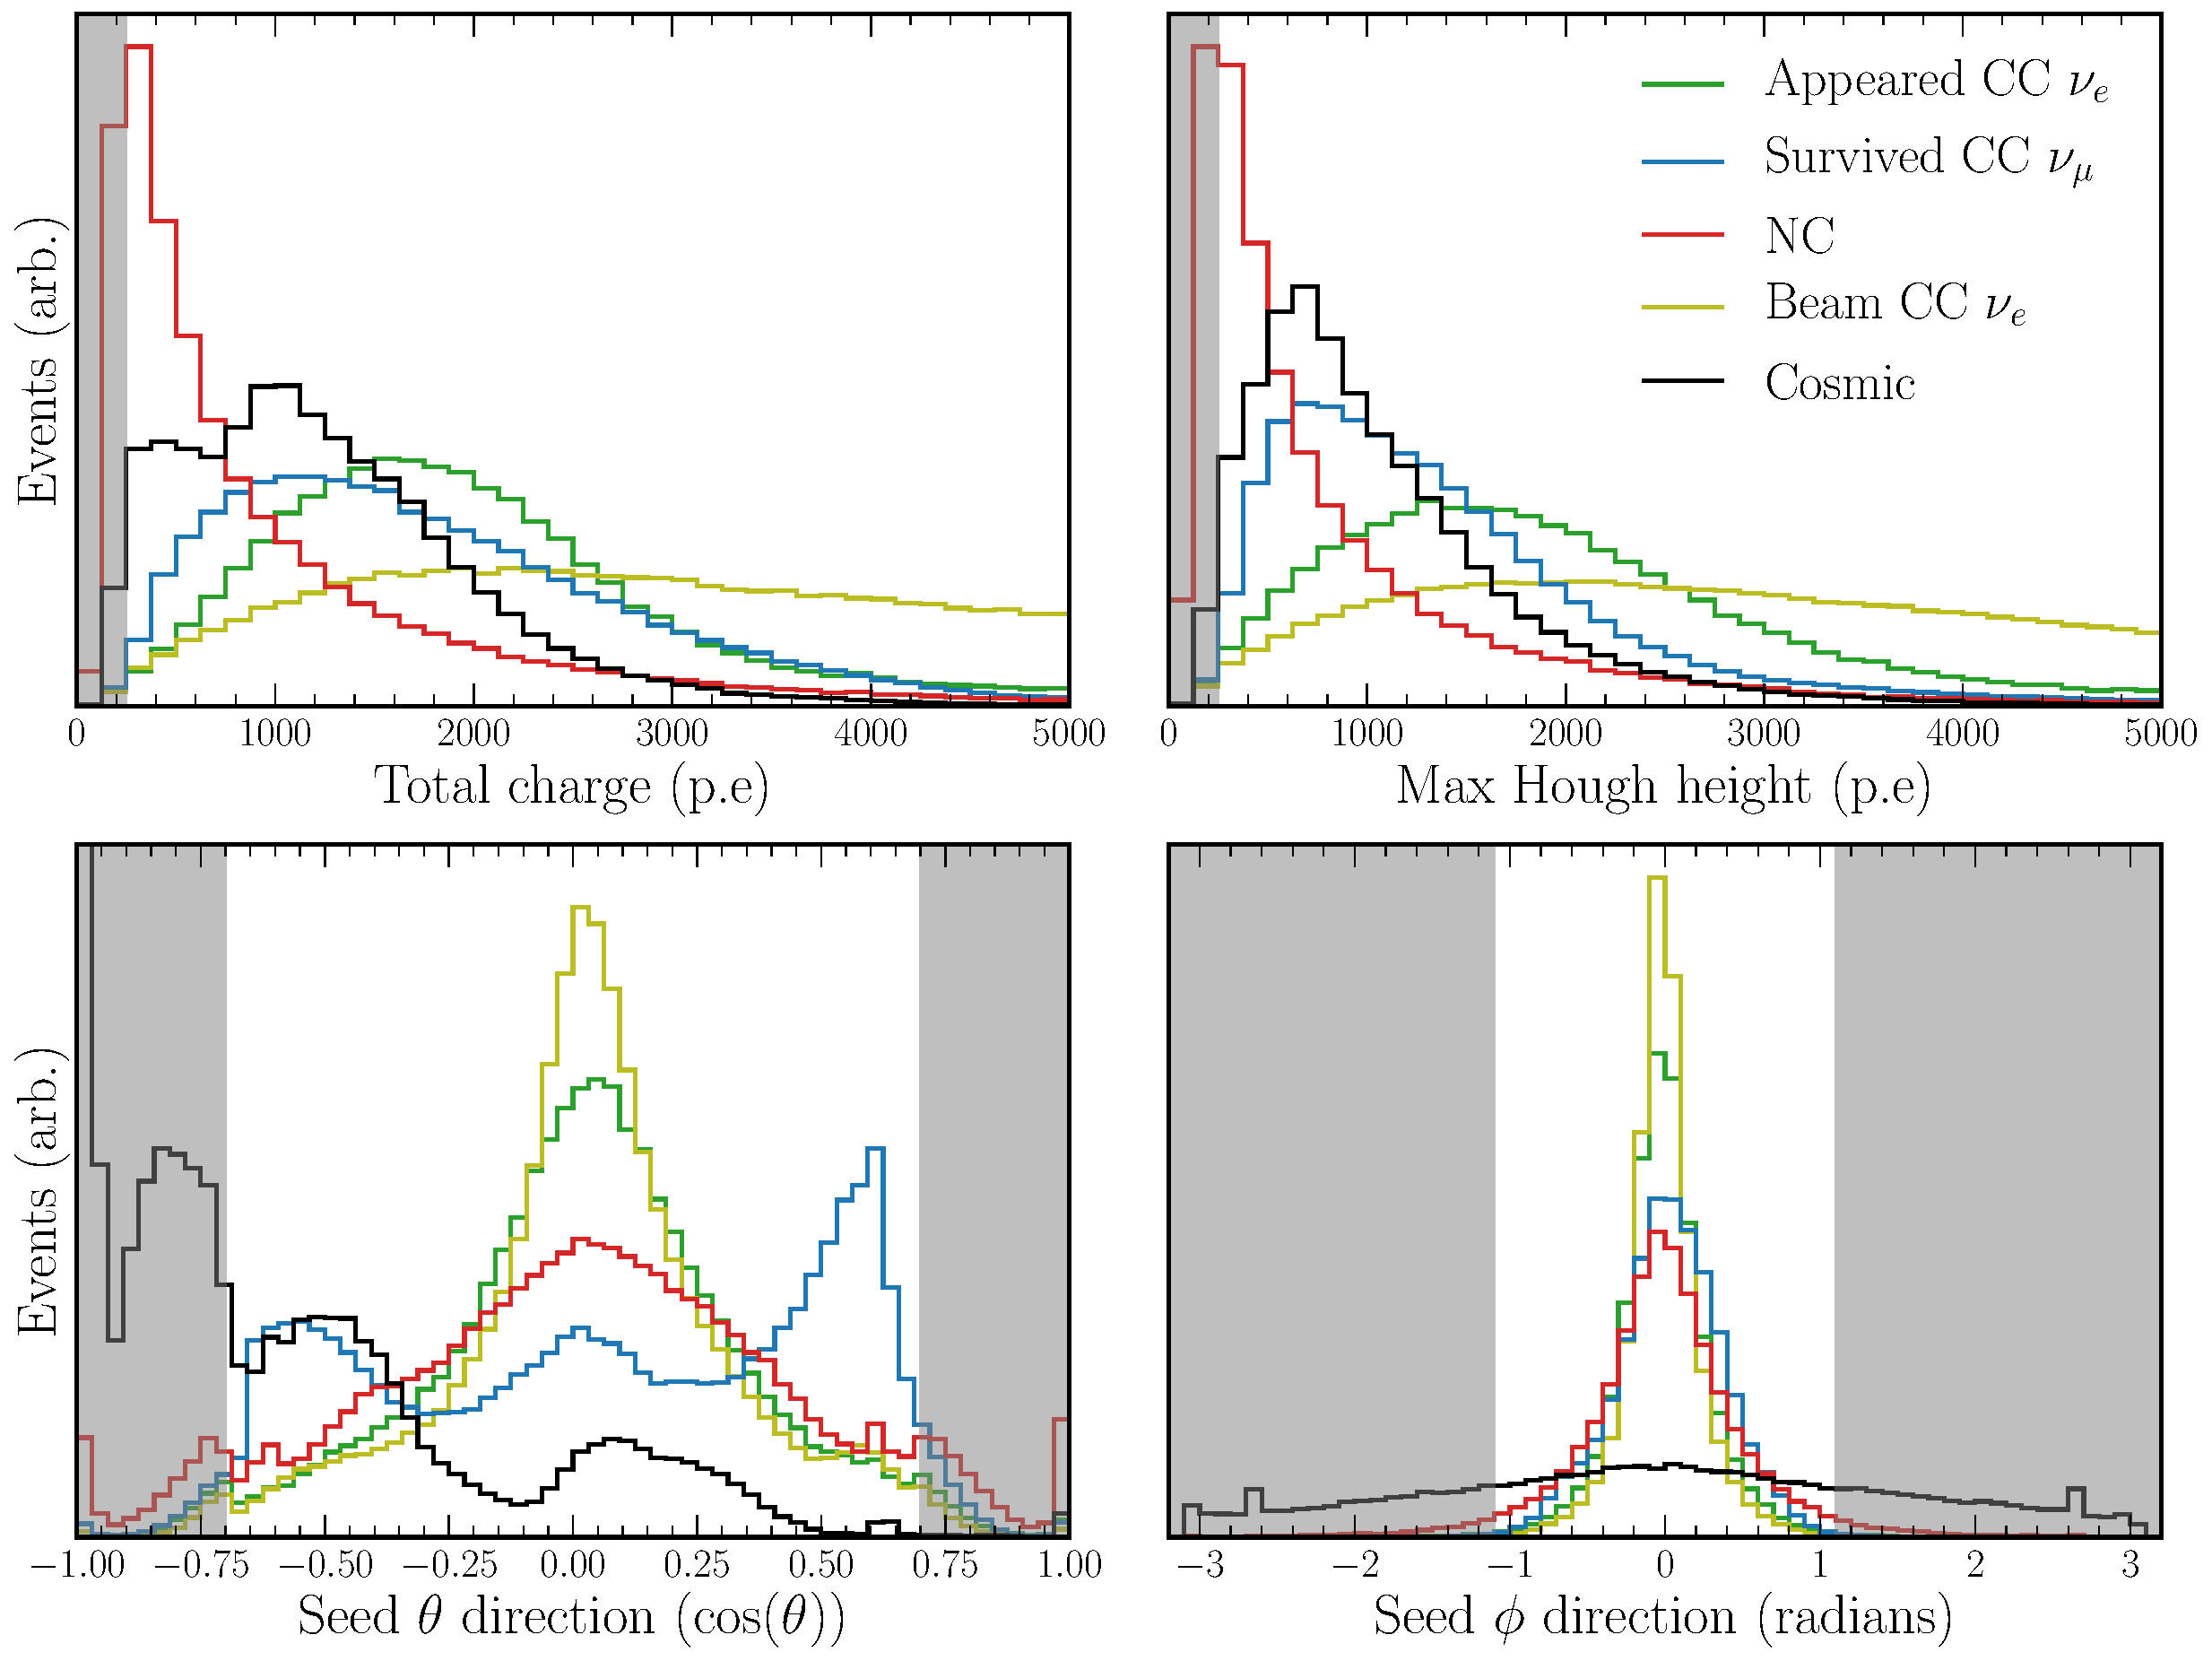
\includegraphics[width=\textwidth]{diagrams/7-results/explore_simple_cuts.pdf}
    \caption[Plots detailing evaluation sample preselection cuts]
    {Plots showing the four simple preselection cuts and how they affect the different event
        categories. The greyed out regions indicate rejected events.}
    \label{fig:explore_simple_cuts}
\end{figure}

\subsection{Cosmic rejection and containment} %%%%%%%%%%%%%%%%%%%%%%%%%%%%%%%%%%%%%%%%%%%%%%%%%%%%
\label{sec:results_eval_cosmic} %%%%%%%%%%%%%%%%%%%%%%%%%%%%%%%%%%%%%%%%%%%%%%%%%%%%%%%%%%%%%%%%%%

The \emph{cosmic score} output from the trained cosmic rejection network gives excellent
separation between beam like (output close to zero) and cosmic like (output close to one) events,
as can be seen in Fig.~\ref{fig:cosmic_outputs}. Importantly, the vast majority of beam events are
associated with a score incredibly close to zero as is more clearly shown in
Fig.~\ref{fig:cosmic_zoomed_outputs}. Given this, a tight cut of a \emph{cosmic score} below
0.0001 is chosen by inspection to select beam like events. Out of the total 350000 cosmic events
in the evaluation sample, all are rejected by this cut alongside preselection. Without the
addition of the second \emph{escapes score} output during training, the cosmic rejection network
instead allows five cosmic events to pass preselection and the cut above.

\begin{figure} % COSMIC OUTPUTS DIAGRAM %
    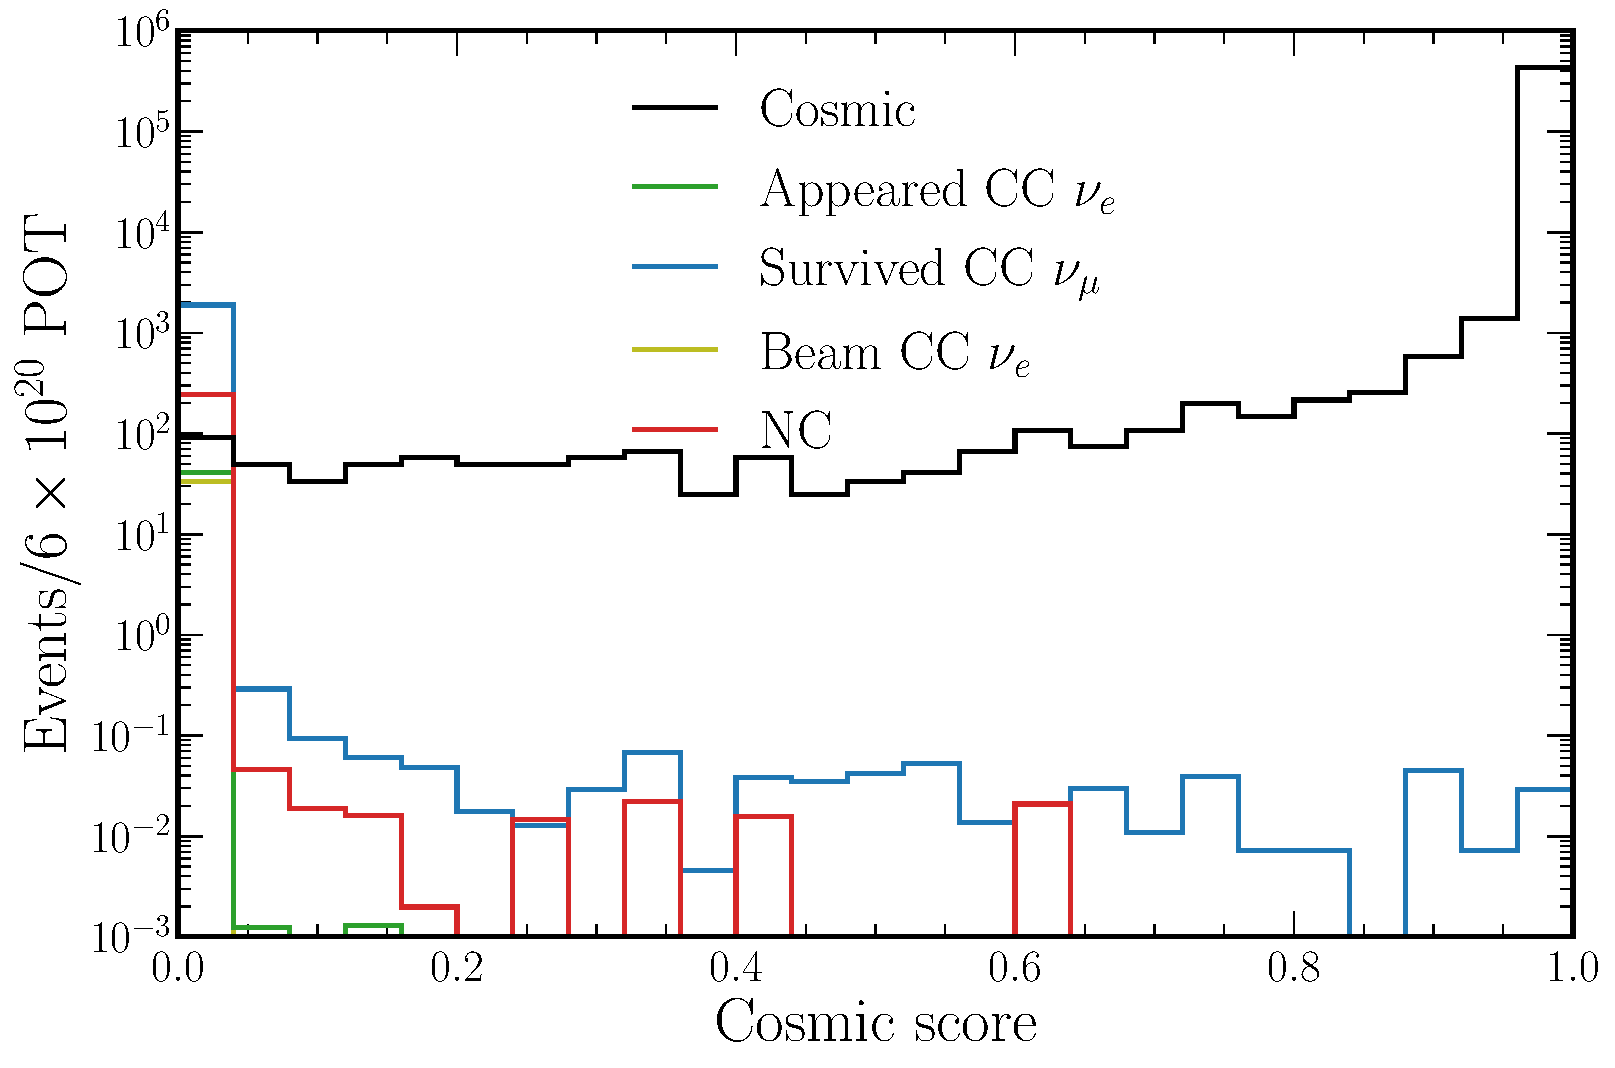
\includegraphics[width=0.7\textwidth]{diagrams/7-results/final_cosmic_outputs.pdf}
    \caption[Distribution of cosmic score output values]
    {Distribution of \emph{cosmic score} output values from the trained cosmic rejection network
        for the different event categories. A score close to one signifies a cosmic like event,
        while a score close to zero corresponds to a beam like event. Only preselected events are
        shown to better highlight the events this output aims to classify.}
    \label{fig:cosmic_outputs}
\end{figure}

\begin{figure} % COSMIC OUTPUTS ZOOMED DIAGRAM %
    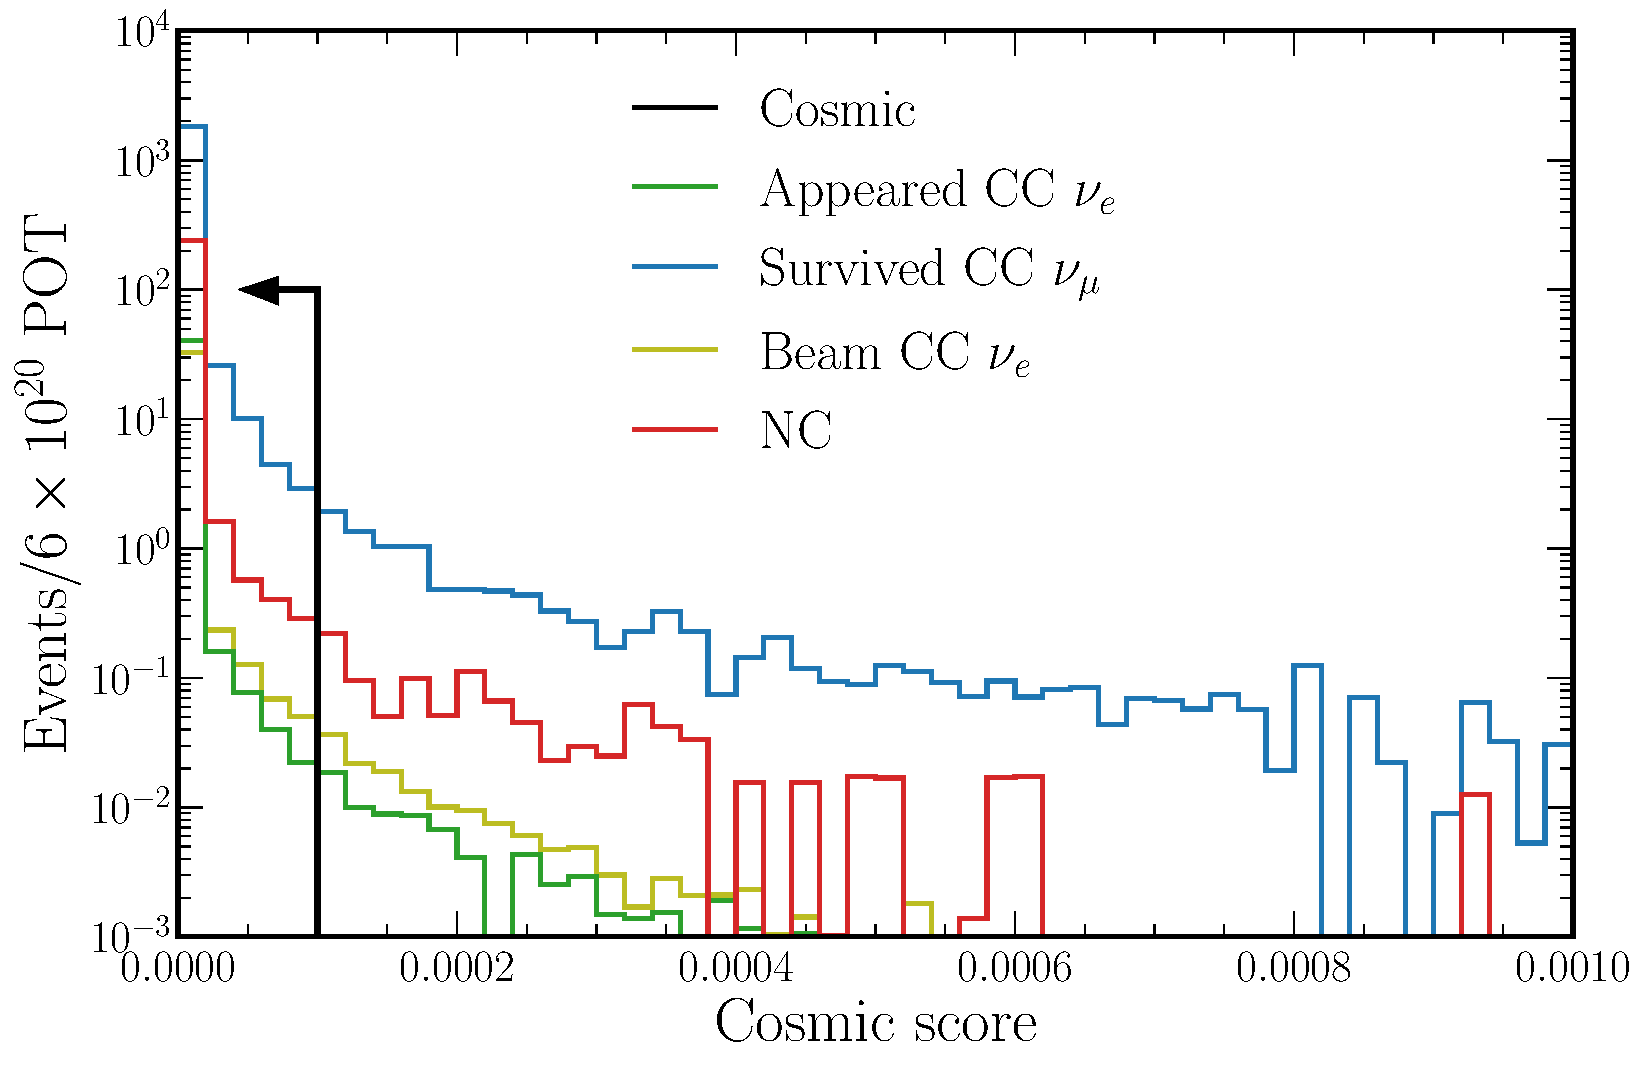
\includegraphics[width=0.7\textwidth]{diagrams/7-results/final_cosmic_zoomed_outputs.pdf}
    \caption[Distribution of cosmic score output values close to zero]
    {Distribution of \emph{cosmic score} output values from the trained cosmic rejection network
        close to zero for the different event categories. The cosmic rejection cut value at 0.0001
        is shown with the arrow indicating selected events. No cosmic events are within the shown
        range due to the statistical limitations of the evaluation sample.}
    \label{fig:cosmic_zoomed_outputs}
\end{figure}

It is crucial for accurate neutrino energy estimation that the activity of an event is fully
contained within the volume of the detector. If charged event particles instead leave the detector
and emit Cherenkov radiation not captured by PMTs, it can be incredibly difficult to estimate the
resulting missing energy and hence neutrino energy. Within the \chipsfive detector, this is
particularly important for CC $\nu_{\mu}$ events for which only 44\% of the long track primary
charged muons are fully contained within the detector volume.

Therefore, the second output from the cosmic rejection network \emph{escapes score} is also used
to select events. Although this only considers the primary charged lepton instead of all particles
in an event, it still acts as a reasonable simplified proxy for event containment. The
distribution of \emph{escapes score} output values from the trained cosmic rejection network is
shown in Fig.~\ref{fig:final_escapes_outputs}.

A value below 0.5 is chosen by inspection to select events for which the primary charged lepton is
fully contained within the detector. With this selection, 97\%(96\%) of CC $\nu_{\mu}$ events for
which the primary charged lepton is contained within(escapes) the detector are classified
correctly, resulting in a 95\% purity for the surviving CC $\nu_{\mu}$ sample. As expected, the
vast majority of CC $\nu_{e}$ and NC events are selected.

For comparison with other experiments, the escapes cut effectively works as a quasi fiducial
volume cut, but just for an energy-dependent region near the downstream wall of the detector.
Fiducial volume cuts are common in neutrino experiments, to remove events whose activity is close
to the detector walls and, therefore, can not be reconstructed well. Future work, should explore
how a fully implemented fiducial cut using the reconstructed interaction vertex position impacts
the final performance.

\begin{figure} % ESCAPES OUTPUTS DIAGRAM %
    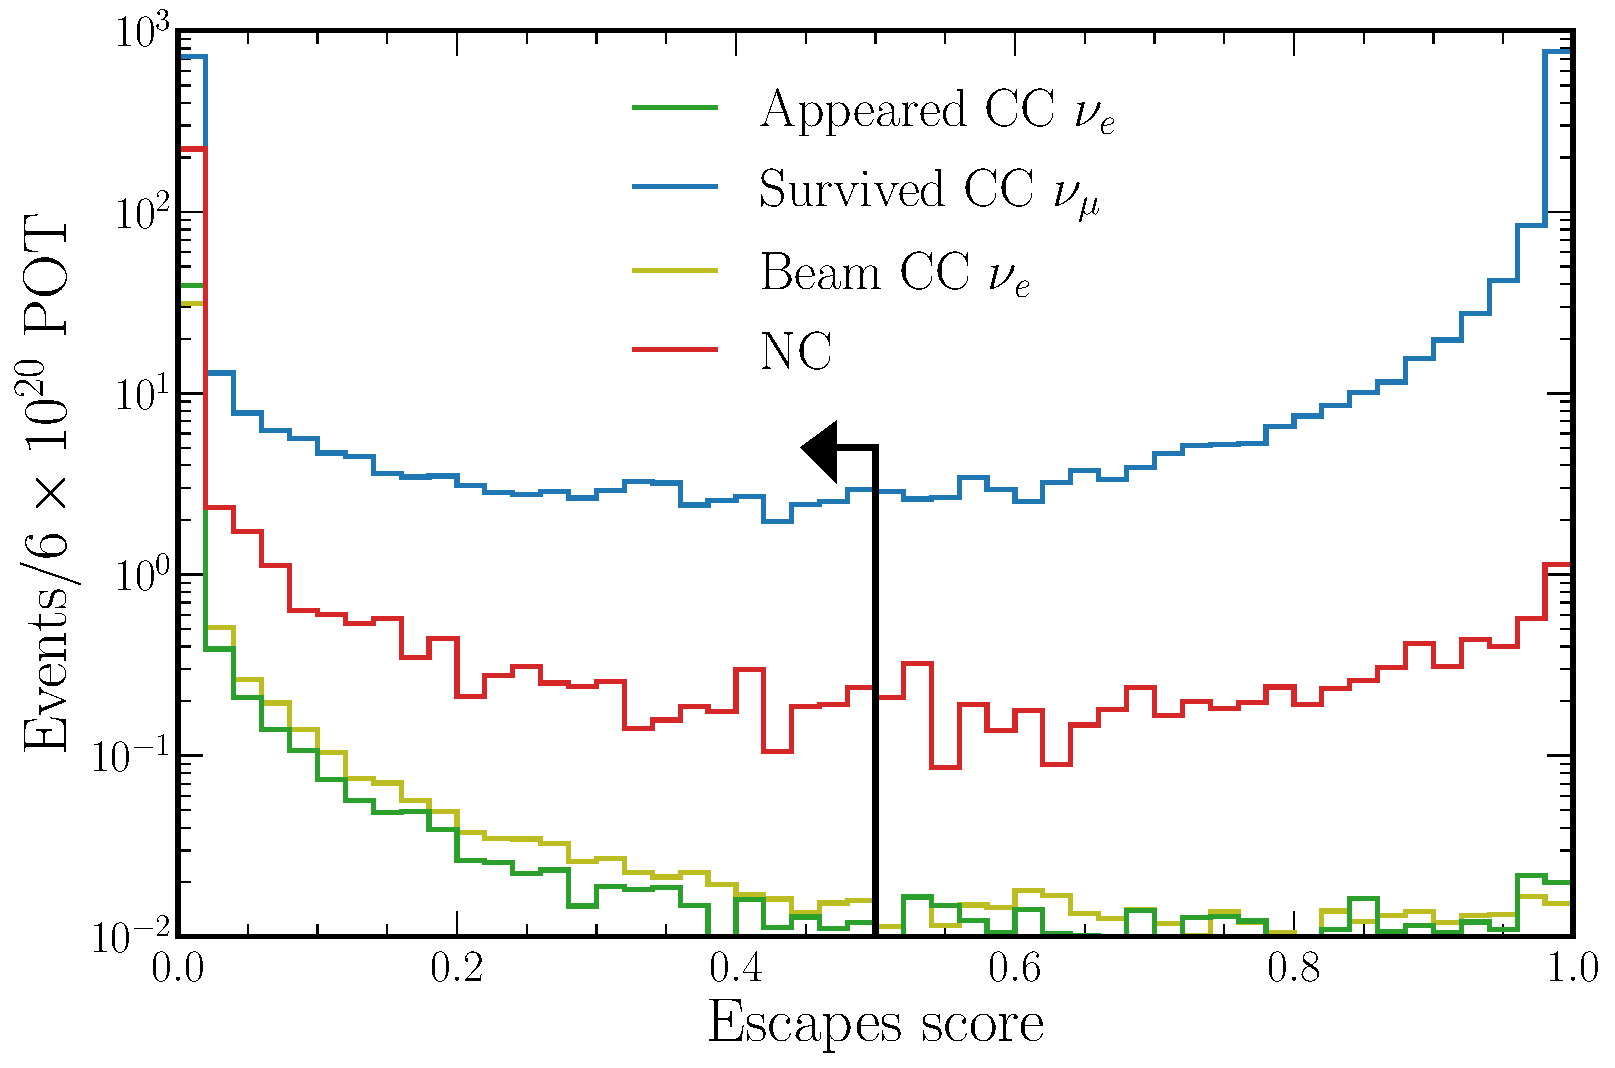
\includegraphics[width=0.7\textwidth]{diagrams/7-results/final_escapes_outputs.pdf}
    \caption[Distribution of escapes score output values]
    {Distribution of \emph{escapes score} output values from the trained cosmic rejection network
        for the different event categories. A score close to one signifies an escaped primary
        charged lepton like event, while a score close to zero corresponds to a contained primary
        charged lepton like event. The containment cut value at 0.5 is shown with the arrow
        indicating the events that are selected.}
    \label{fig:final_escapes_outputs}
\end{figure}

The total number of expected events per year that pass each successive cut (including
preselection) for each event category is shown in Table.~\ref{tab:selection}. Both CC $\nu_{e}$
categories are selected with an efficiency greater than 90\%, while CC $\nu_{\mu}$ events are
intentionally reduced to 40\% efficiency to ensure they are fully contained. Furthermore, NC
events are found to be primarily rejected by the preselection, while cosmic events are heavily
rejected by both the preselection and \emph{cosmic score} cuts.

\begin{table}
    \begin{tabular}{lccccc}
                       & App CC $\nu_{e}$ & CC $\nu_{\mu}$ & Beam CC $\nu_{e}$ & NC             & Cosmic                 \\
        \midrule
        Total events   & 44.2             & 2045.9         & 35.1              & 348.7          & 1211000                \\
        + preselection & 41.2             & 1889.5         & 33.5              & 239.6          & 249260                 \\
        + cosmic cut   & 41.1             & 1874.4         & 33.4              & 238.0          & 0.13                   \\
        + escapes cut  & 40.8             & 818.0          & 33.0              & 231.0          & 0.02                   \\
        \midrule
        Efficiency     & $92.4\pm0.4\%$   & $40.0\pm0.2\%$ & $94.2\pm0.4\%$    & $66.3\pm0.7\%$ & $\sim1.5\times10^{-8}$ \\
    \end{tabular}
    \caption[Number of events passing basic cuts for each event category.]
    {The total number of events and the number that pass successive selection cuts for the
        different event categories. The preselection, \emph{cosmic score} cut, and \emph{escapes
            score} cut numbers are shown.}
    \label{tab:selection}
\end{table}

When compared to the approximately 2.1 million expected cosmic events per year, the zero selected
out of 350000 evaluation events is not statistically significant. However, the generation of a
sufficiently sized cosmic evaluation sample is deemed infeasible due to the vast computational
resources and time required.

Therefore, to more accurately gauge the number of cosmic events likely to be classified as beam
events, we consider the more statistically significant number that passes a loose \emph{cosmic
    score} cut below a value of $0.9$. In this case, when combined with the preselection and
\emph{escapes score} cut, $38$ out of $350000$ evaluation sample cosmic events are selected, which
when weighted gives to $317$ events per year. Assuming a flat distribution of events between a
\emph{cosmic score} of zero and $0.9$, and using the actual $0.0001$ cut value, $0.035$ events are
expected to be selected. This corresponds to an excellent combined rejection factor for cosmic
muon events of $\sim1.5\times10^{-8}$.

Additionally, of the $317$ events under a \emph{cosmic score} value of $0.9$, $167$ would be
selected as CC $\nu_{\mu}$ and zero as CC $\nu_{e}$ by the beam classification detailed in the
following subsection. This gives high confidence that even if a tiny number of cosmic events are
selected, they would be classified as CC $\nu_{\mu}$ and not contaminate the principle CC
$\nu_{e}$ selection. In summary, the expected cosmic muon contamination of the final beam
selections is expected to be negligible and ignored for the rest of this results section. When
compared to the approximately $2\%$ cosmic contamination of the CC $\nu_{\mu}$ sample seen by
\nova~\cite{acero2019}, the performance is apparent.

\subsection{Beam classification} %%%%%%%%%%%%%%%%%%%%%%%%%%%%%%%%%%%%%%%%%%%%%%%%%%%%%%%%%%%%%%%%%
\label{sec:results_eval_beam} %%%%%%%%%%%%%%%%%%%%%%%%%%%%%%%%%%%%%%%%%%%%%%%%%%%%%%%%%%%%%%%%%%%%

The output values from each of the \emph{combined category} neurons of the trained beam
classification network give the probability score that an event belongs to the corresponding
category. As the output neuron scores collectively sum to one, the highest-scoring neuron can be
used to classify events as either CC $\nu_{e}$, CC $\nu_{\mu}$, or NC in nature.
Fig.~\ref{fig:final_comb_cat_confusion} shows the resulting classification matrix using this
approach.

\begin{figure} % FINAL COMB CAT CONFUSION DIAGRAM %
    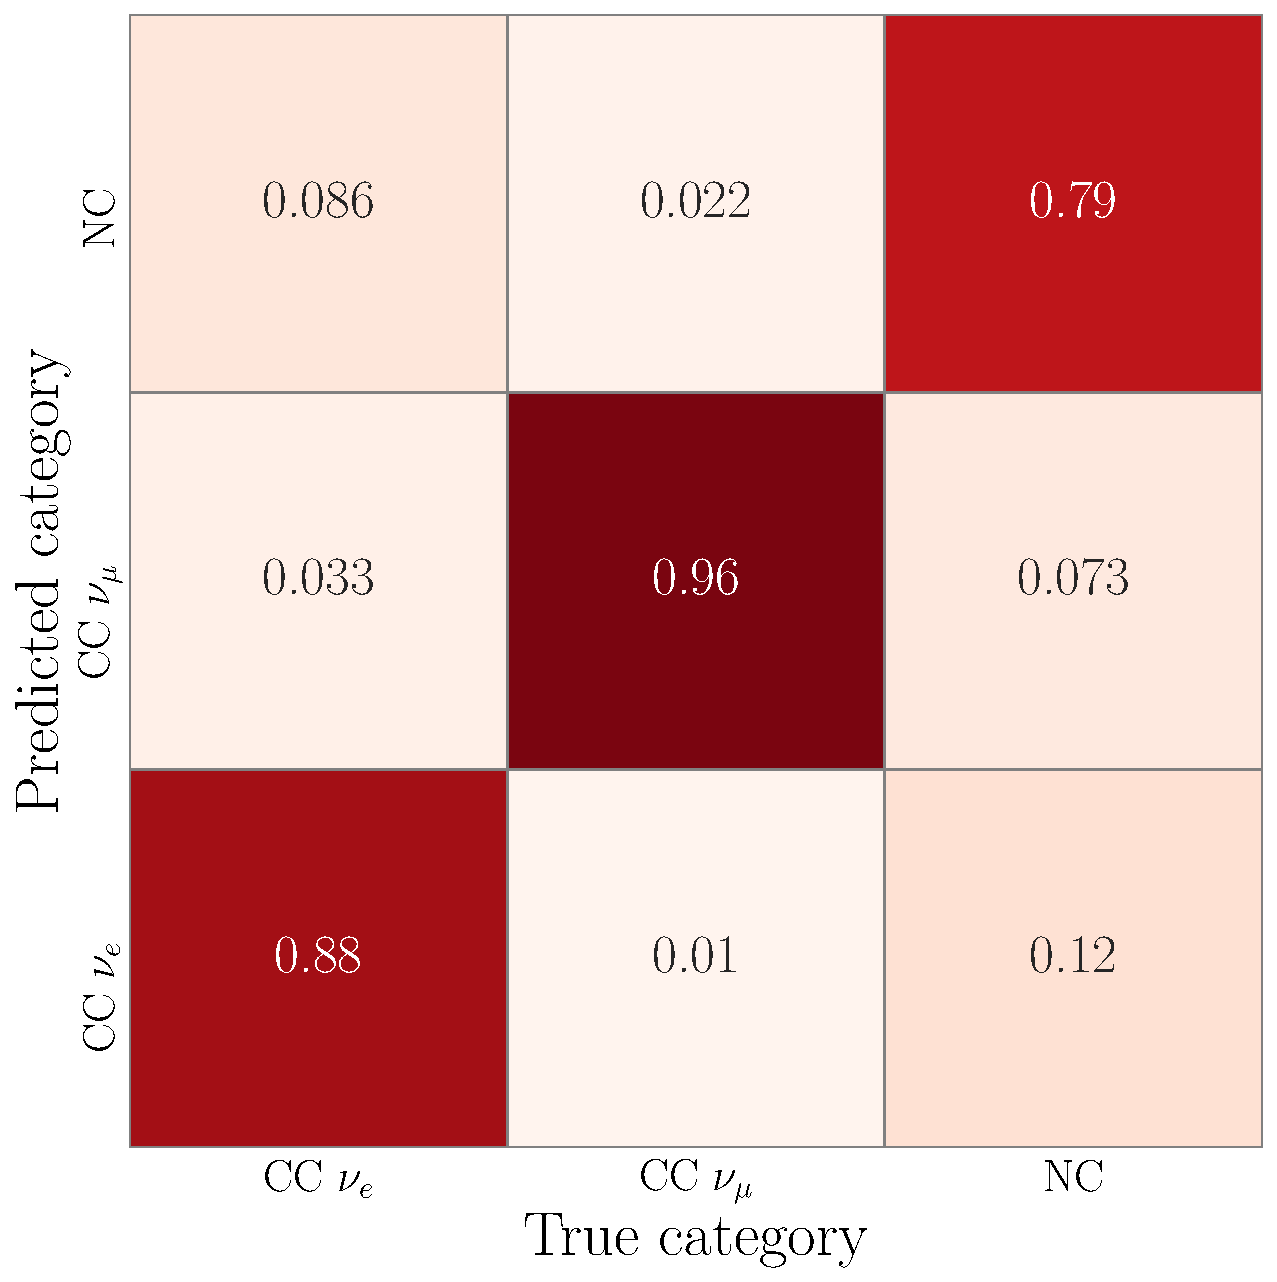
\includegraphics[width=0.6\textwidth]{diagrams/7-results/final_comb_cat_confusion.pdf}
    \caption[Classification matrix for the combined category output of the beam classification
        network] {Classification matrix for the \emph{combined category} output of the trained
        beam classification network. Events are simply classified using the categorical score for
        which they have the highest value. The numbers shown are the fraction of true category
        events classified into each of the three possible categories.}
    \label{fig:final_comb_cat_confusion}
\end{figure}

To access the beam classification performance more rigorously it is instead common to calculate a
selection score for each of the output categories, found by maximising a figure-of-merit (FOM).
All events with a score above this optimised value are then accepted as signal. In this work, the
figure-of-merit, $\mathrm{efficiency}\times\mathrm{purity}$ is optimised. Below the results for
both appeared CC $\nu_{e}$ and survived CC $\nu_{\mu}$ selections are presented.

\subsubsection*{CC $\nu_{e}$ selection} %%%%%%%%%%%%%%%%%%%%%%%%%%%%%%%%%%%%%%%%%%%%%%%%%%%%%%%%%%

The distribution of CC $\nu_{e}$ scores for the different event categories is shown in
Fig.~\ref{fig:final_beam_nuel_outputs}. Strong separation between appeared CC $\nu_{e}$ signal and
both CC $\nu_{\mu}$ and NC background events is achieved, especially given the large difference in
sample size. As no attempt is made to separate the appeared CC $\nu_{e}$ signal component from the
intrinsic beam CC $\nu_{e}$ background, both are clustered with scores close to one as expected.

\begin{figure} % BEAM OUTPUTS NUEL DIAGRAM %
    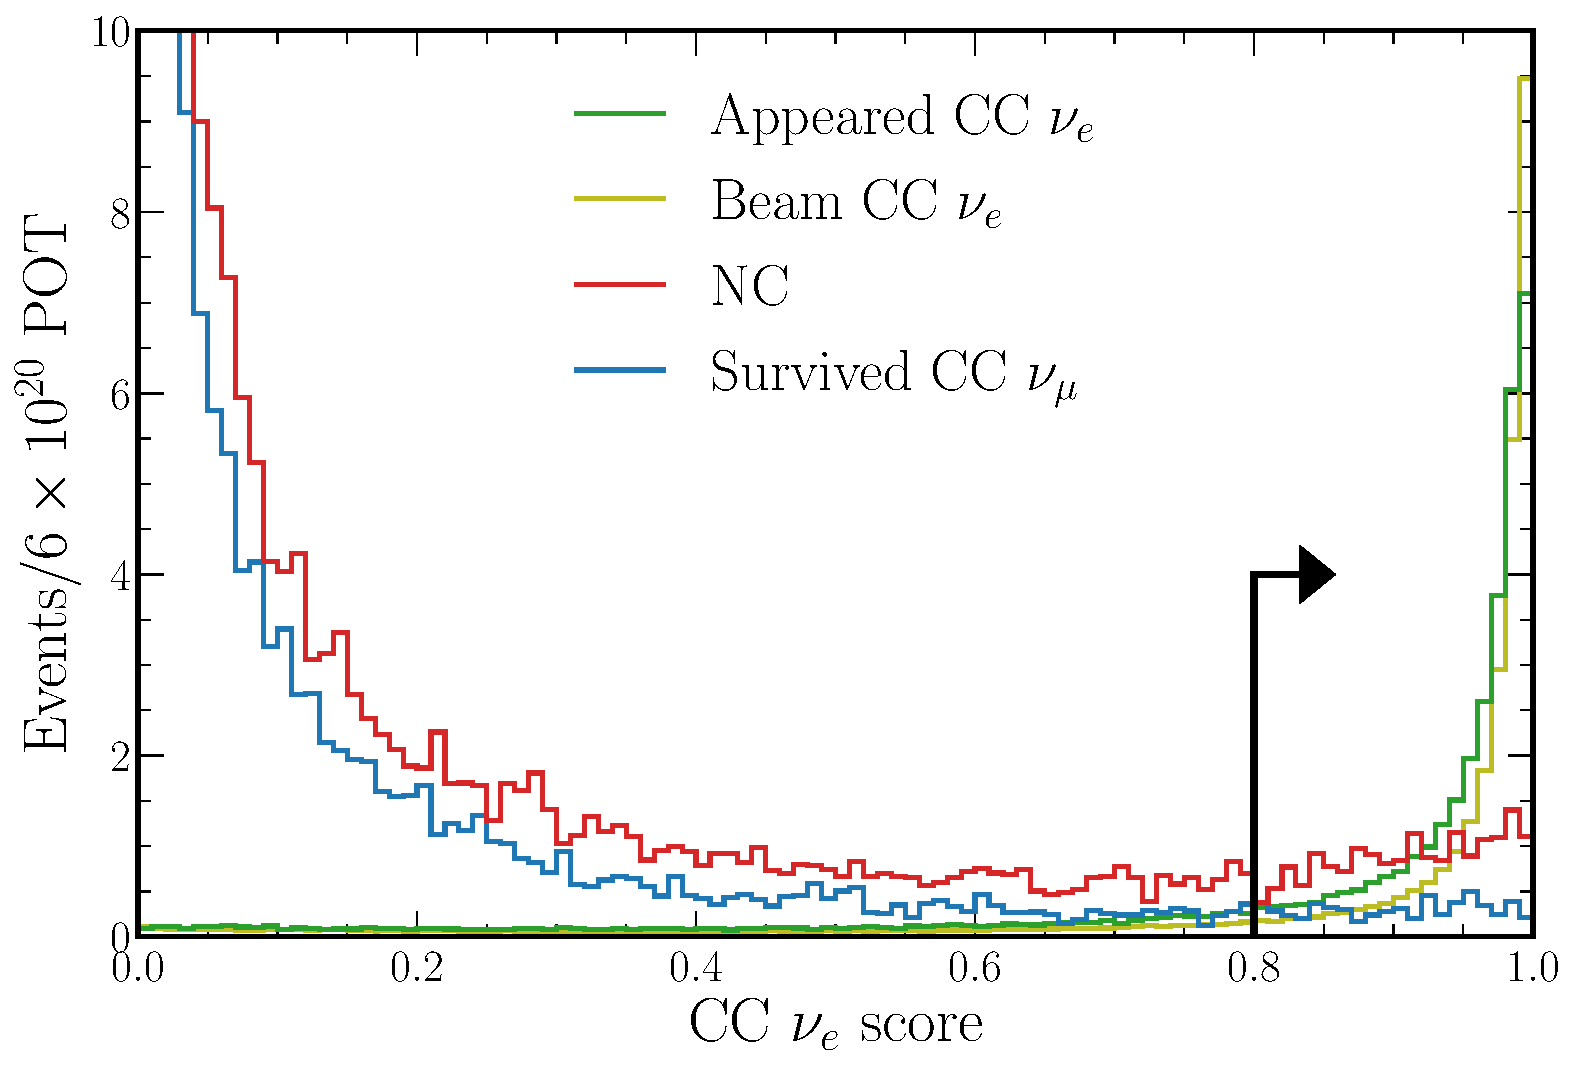
\includegraphics[width=0.7\textwidth]{diagrams/7-results/final_beam_nuel_outputs.pdf}
    \caption[Distribution of CC $\nu_{e}$ scores from the trained beam classification network]
    {Distribution of \emph{combined category} CC $\nu_{e}$ scores from the trained beam
        classification network for the different event categories. A score close to one signifies
        a CC $\nu_{e}$ like event. The y-axis has been truncated so that the CC $\nu_{\mu}$ and NC
        components are not fully visible in order to better show the distribution of signal CC
        $\nu_{e}$ events.}
    \label{fig:final_beam_nuel_outputs}
\end{figure}

The efficiency, purity, and their product (the figure-of-merit) for CC $\nu_{e}$ events (both
appeared and beam) as a function of selecting events above a certain CC $\nu_{e}$ score are shown
in Fig.~\ref{fig:final_nuel_eff_curves}. $\mathrm{Efficiency}\times\mathrm{purity}$ is optimised
by selecting events with a CC $\nu_{e}$ score above $0.8$, achieving a value of $0.519$. Note that
$\mathrm{efficiency}\times\mathrm{purity}$ is optimised considering both appeared and beam CC
$\nu_{e}$ components as signal. Due to their indistinguishable nature, this is the only reasonable
approach to generate cut values.

The corresponding number and efficiency of selected events for each event category, as well as the
appeared signal CC $\nu_{e}$ purity, is shown in Table.~\ref{tab:nuel_selection}. The final FOM
selected signal purity of $38.3\pm0.5\%$ may appear low, but this is mainly due to the
indistinguishable intrinsic beam CC $\nu_{e}$ contamination. When both CC $\nu_{e}$ components are
considered signal the selection purity becomes $71.0\pm0.6\%$.

\begin{figure} % FINAL NUEL EFF CURVES DIAGRAM %
    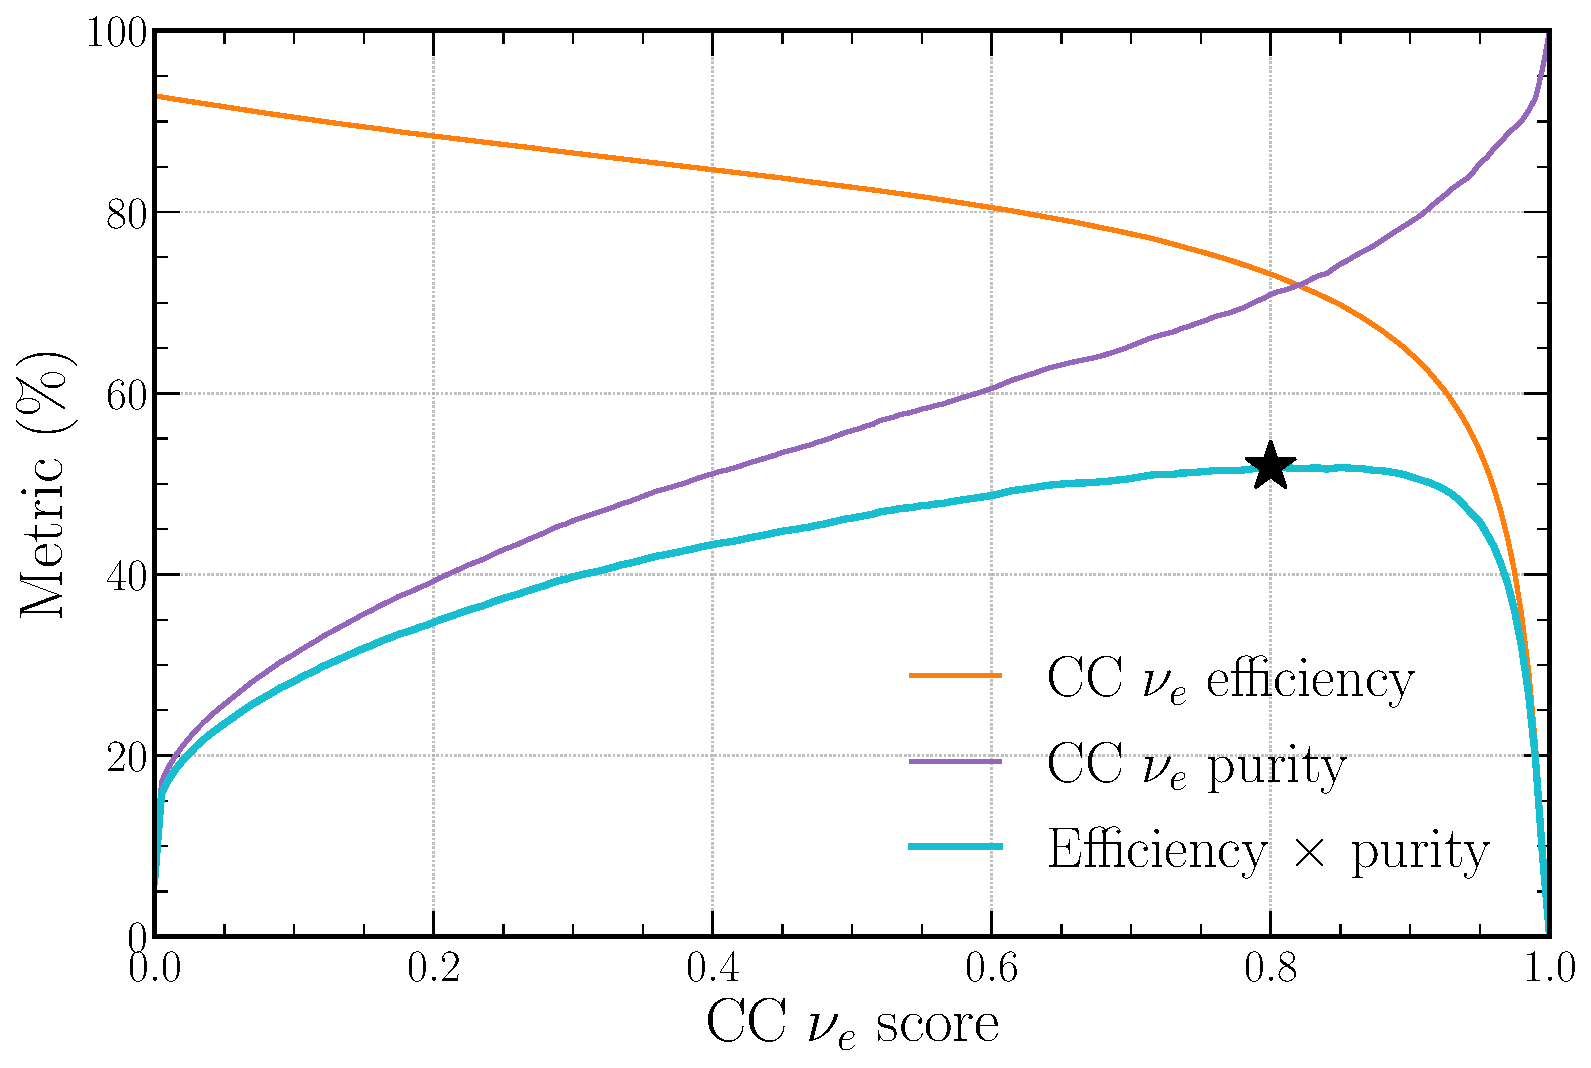
\includegraphics[width=0.7\textwidth]{diagrams/7-results/final_nuel_eff_curves.pdf}
    \caption[CC $\nu_{e}$ efficiency, purity and $\mathrm{efficiency}\times\mathrm{purity}$]
    {CC $\nu_{e}$ efficiency, purity and $\mathrm{efficiency}\times\mathrm{purity}$ for different
        values of CC $\nu_{e}$ score selection.}
    \label{fig:final_nuel_eff_curves}
\end{figure}

\begin{table}
    \begin{tabular}{ccccccc}
                 & CC $\nu_{e}$ sig & Beam CC $\nu_{\mu}$ bkg & CC $\nu_{e}$ bkg & NC bkg        & Sig Purity     \\
        \midrule
        Cuts Num & 40.8             & 818.0                   & 33.0             & 231.0         & $3.6\pm0.1\%$  \\
        FOM Num  & 31.3             & 6.1                     & 26.7             & 17.6          & $38.3\pm0.5\%$ \\
        \midrule
        FOM Eff  & $70.9\pm0.4\%$   & $0.3\pm0.02\%$          & $76.3\pm0.3\%$   & $5.1\pm0.2\%$ & -              \\
    \end{tabular}
    \caption[Table showing CC $\nu_{e}$ selected event numbers, efficiencies and signal purity.]
    {Table showing CC $\nu_{e}$ selected event numbers and corresponding efficiencies for the
        various event categories as well as the associated signal purity. Shown are the numbers
        for both the post preselection, \emph{cosmic score} cut, and \emph{escapes score} cut
        numbers (Cuts) in addition to the $\mathrm{efficiency}\times\mathrm{purity}$ optimised
        (FOM) selection for which the efficiency is shown.}
    \label{tab:nuel_selection}
\end{table}

The $\mathrm{efficiency}\times\mathrm{purity}$ optimised CC $\nu_{e}$ selection efficiency as a
function of energy for the different event categories is shown in Fig.~\ref{fig:final_nuel_hists}.
From low neutrino energies, both CC $\nu_{e}$ category selection efficiencies rise steeply to a
plateau of approximately 80\% beginning at \unit{4}{GeV}. This is expected as low energy CC
$\nu_{e}$ events typically do not have well-defined electron Cherenkov rings, leading to their
rejection. Due to the abundance of selected intrinsic beam CC $\nu_{e}$ events at higher energies,
the appeared CC $\nu_{e}$ purity is observed to peak at approximately \unit{2.5}{\GeV} (close to
the oscillation maximum) before declining. The NC efficiency is seen to slowly increase
approaching 15\% for hadronic component energies above \unit{5}{\GeV}; this is likely due to
misidentification of high energy pions or protons as electrons. Importantly, however, within the
key signal region from 2 to \unit{4}{\GeV}, NC selection efficiency remains low.

\begin{figure} % FINAL NUEL HISTS DIAGRAM %
    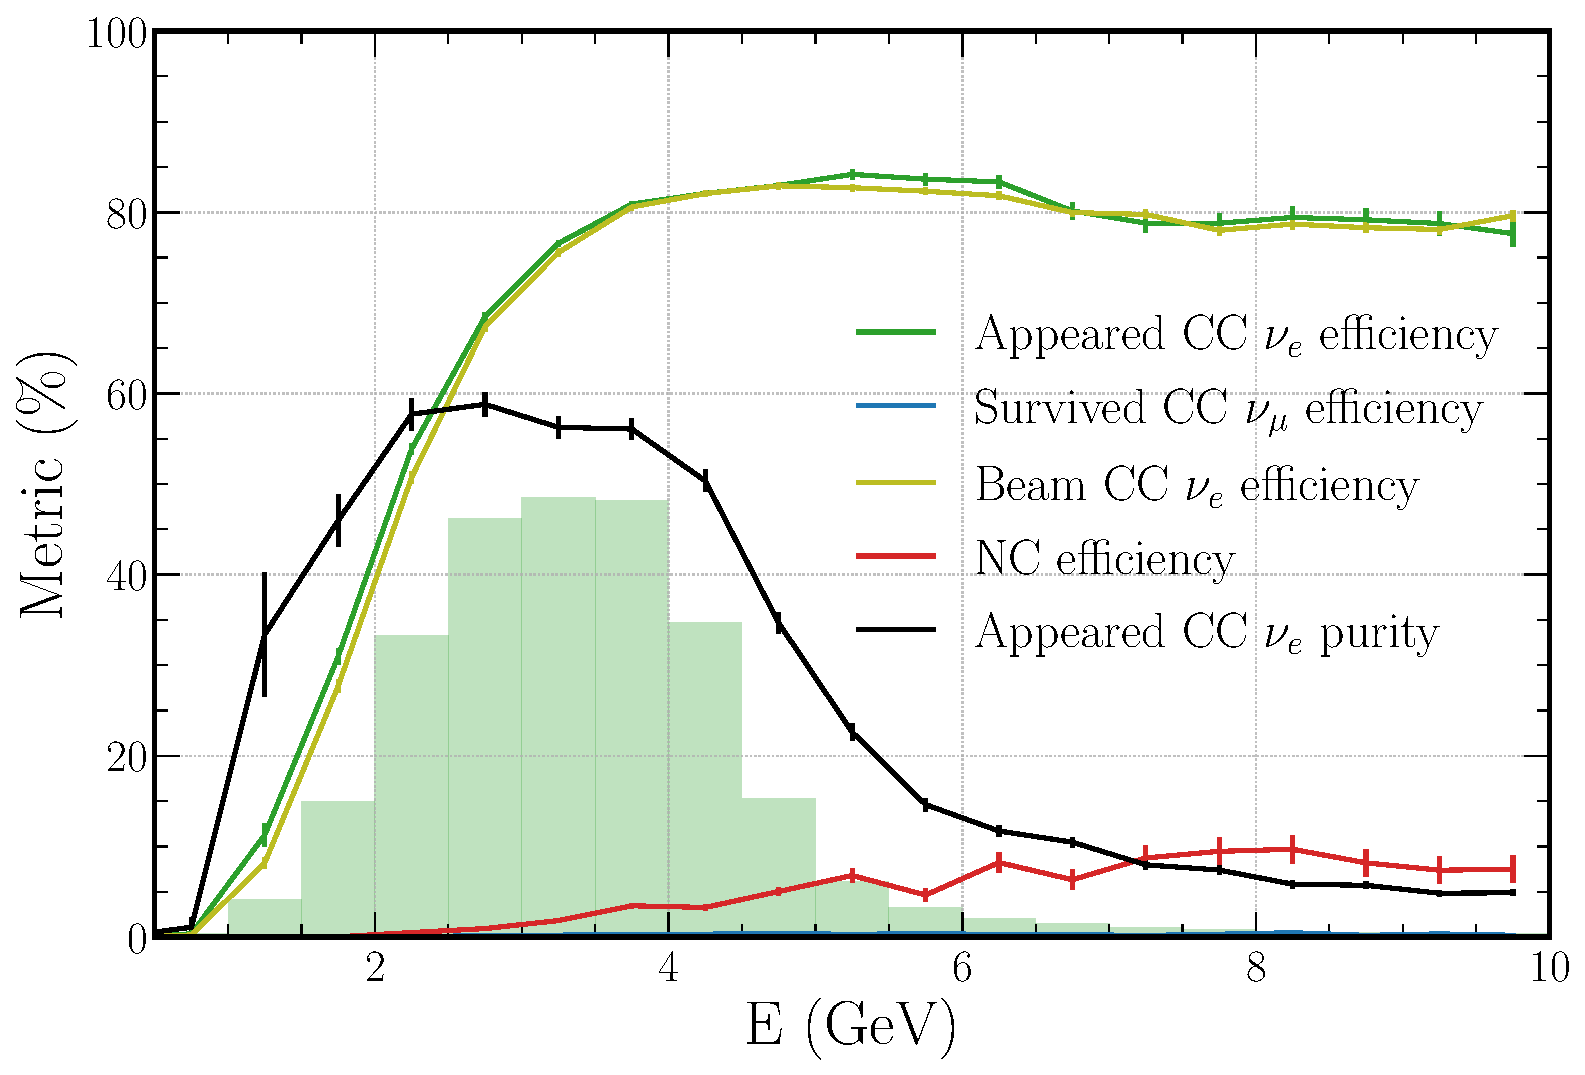
\includegraphics[width=0.7\textwidth]{diagrams/7-results/final_nuel_hists.pdf}
    \caption[Efficiency of CC $\nu_{e}$ selection as a function of energy]
    {Efficiency of CC $\nu_{e}$ selection for the different event categories as well as appeared CC
        $\nu_{e}$ purity as a function of energy. All CC categories are shown in terms of neutrino
        energy, while NC events are shown in terms of the hadronic component energy. The survived CC
        $\nu_{\mu}$ efficiency is so low it is barely visible near zero. For reference, the true
        appeared CC $\nu_{e}$ neutrino energy distribution is shown in the green.}
    \label{fig:final_nuel_hists}
\end{figure}

The best way to understand the relative performance of the CNN CC $\nu_{e}$ classification is by
comparison with the standard event selection presented in Section.~\ref{sec:cnn_old_pid}. The
distribution of output scores from both neural networks used in the standard selection is shown in
Fig.~\ref{fig:final_old_pid_outputs}. By optimising the selection values for both networks, 0.91
and 0.78 respectively, to maximise $\mathrm{efficiency}\times\mathrm{purity}$, the standard CC
$\nu_{e}$ selection sample is found. All events that pass the preselection, not just those shown
in Fig.~\ref{fig:final_old_pid_outputs} are used in this optimisation.

A maximum $\mathrm{efficiency}\times\mathrm{purity}$ of 0.132 is achieved; only 25\% the value
reached by the CNN approach. Both the signal efficiency of 34\% compared to 71\% and combined
appeared and beam CC $\nu_{e}$ purity of 39\% compared to 71\% are considerably lower than that
provided by the new CNN classification. Furthermore, the signal efficiency of 71\% compares well
to the 62\%(64\%) achieved by the \nova(T2K) selection. However, the purity is significantly lower
at 38\% compared to the 78\%(80\%) reached by \nova(T2K)~\cite{acero2019, abe2015}.

A large proportion of this difference can be explained by the lower neutrino energies close the
$\sim$\unit{1.5}{\GeV} $\nu_{\mu}\rightarrow\nu_{e}$ oscillation maximum at which these
experiments operate. Firstly, this increases the proportion of easy to identify CC QEL events that
these experiments see. Secondly, the indistinguishable intrinsic beam CC $\nu_{e}$ component that
these experiments see is also lower. However, some of the difference will be due to the `cheap as
chips' philosophy.

\begin{figure} % FINAL OLD PID OUTPUTS DIAGRAM %
    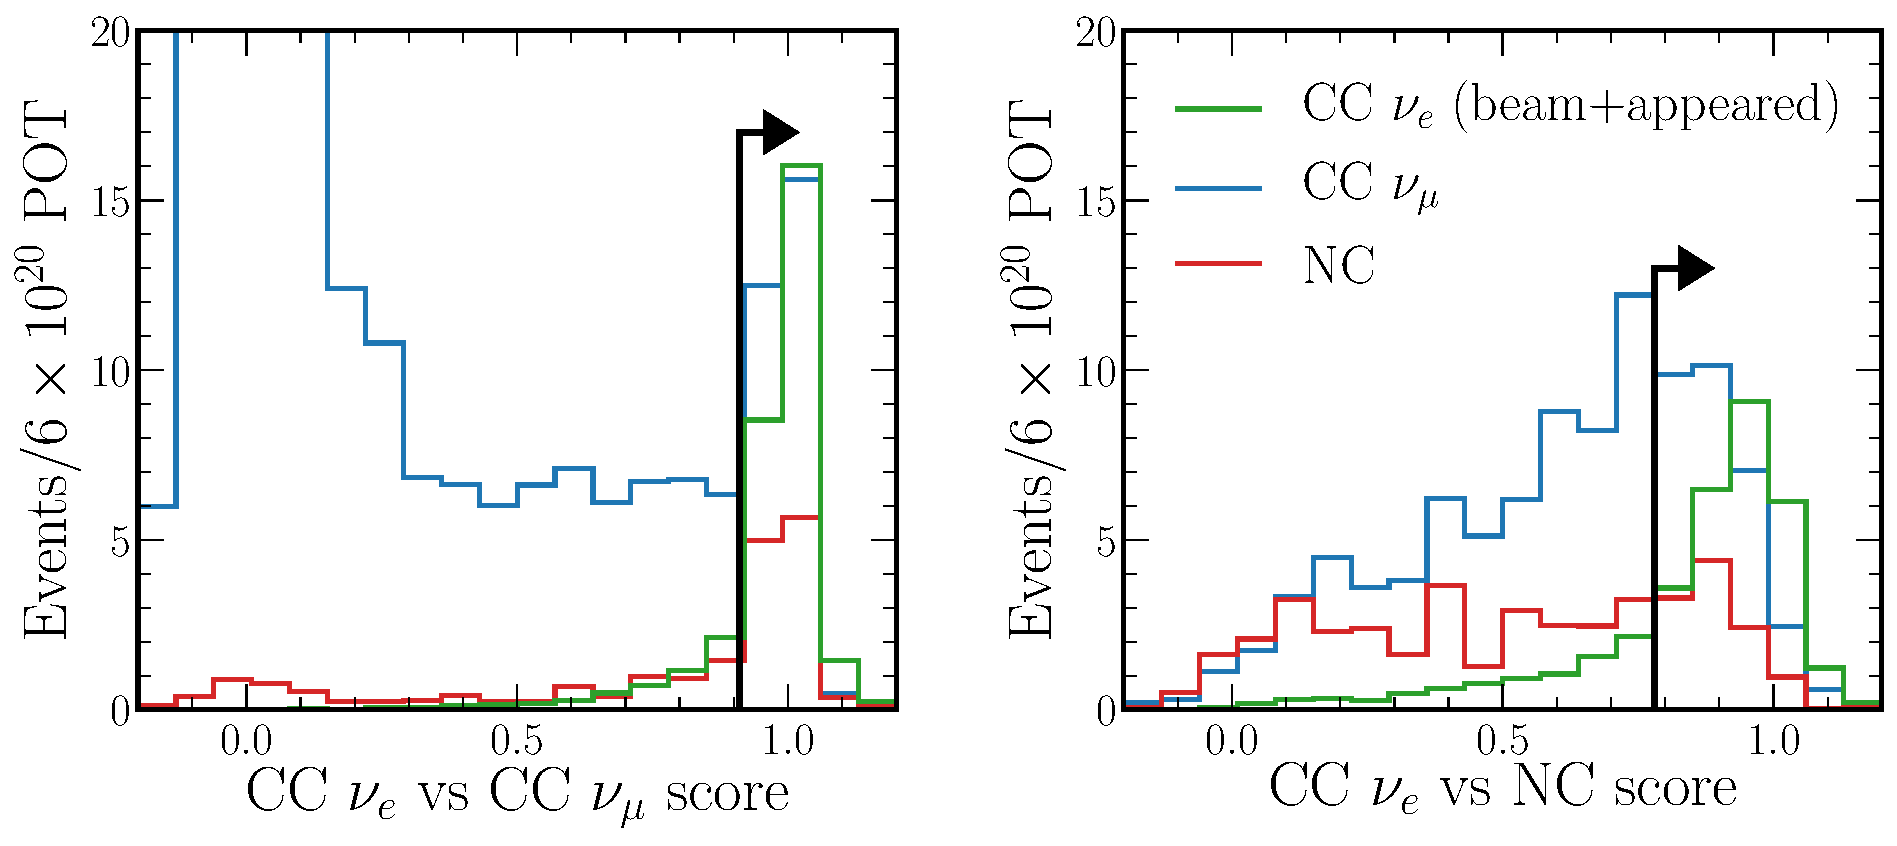
\includegraphics[width=0.8\textwidth]{diagrams/7-results/final_old_pid_outputs.pdf}
    \caption[Distributions of standard event selectio neural network output scores]
    {Distributions of CC $\nu_{e}$ vs CC $\nu_{\mu}$ (left) and CC $\nu_{e}$ vs NC (right) output
        scores from the two standard event selection neural networks for the different event
        categories. A score close to one signifies a CC $\nu_{e}$ like event in both cases. Each
        plot shows events which have passed both the preselection and the optimised cut from the
        other network. This is done to better show the events which the network in question
        rejects. Selected CC $\nu_{e}$ events are shown by the arrows. The y-axis for the CC
        $\nu_{e}$ vs CC $\nu_{\mu}$ distributions has been truncated so that the CC $\nu_{\mu}$
        component is not fully visible in order to better show the distribution of signal CC
        $\nu_{e}$ events. Due to the long reconstruction time required, a smaller but comparable
        evaluation sample is used here.}
    \label{fig:final_old_pid_outputs}
\end{figure}

\subsubsection*{CC $\nu_{\mu}$ selection} %%%%%%%%%%%%%%%%%%%%%%%%%%%%%%%%%%%%%%%%%%%%%%%%%%%%%%%%

The distribution of CC $\nu_{\mu}$ scores for the different event categories is shown in
Fig.~\ref{fig:final_beam_numu_outputs}. Excellent separation between appeared CC $\nu_{\mu}$
signal and both CC $\nu_{e}$ components and NC background is achieved. For high CC $\nu_{\mu}$
scores the difference between signal and background event counts is approximately three orders of
magnitude.

\begin{figure} % BEAM OUTPUTS NUMU DIAGRAM %
    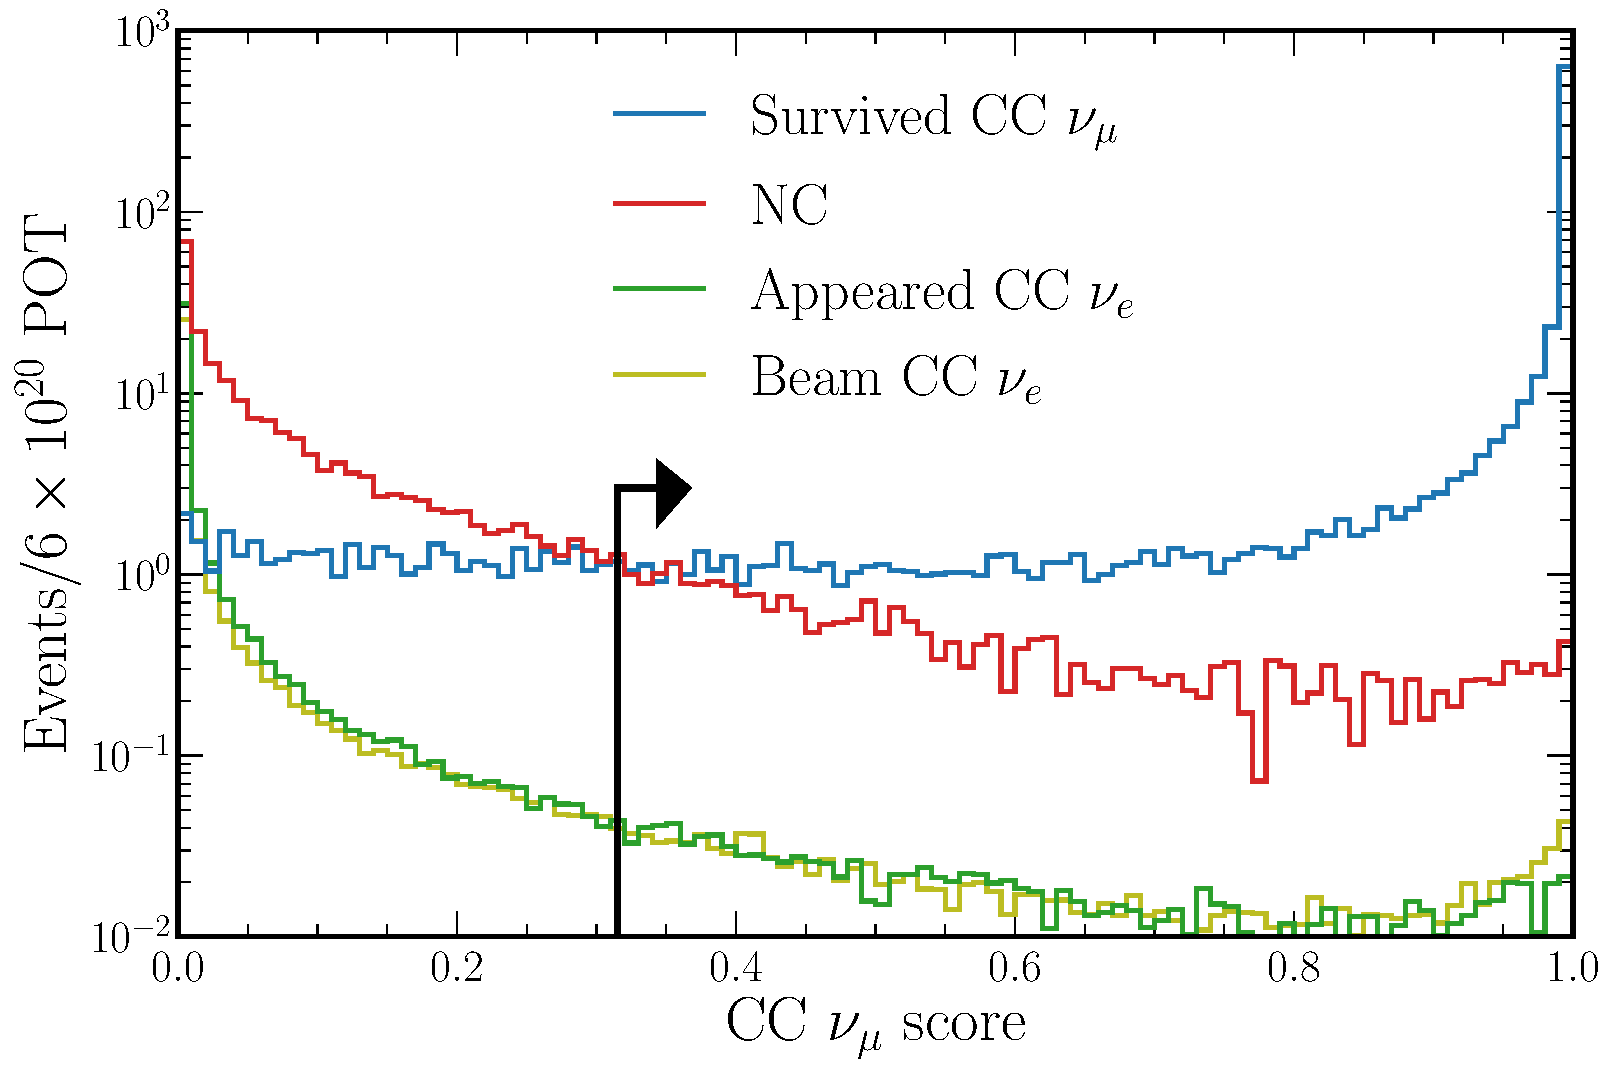
\includegraphics[width=0.7\textwidth]{diagrams/7-results/final_beam_numu_outputs.pdf}
    \caption[Distribution of CC $\nu_{\mu}$ scores from the trained beam classification network]
    {Distribution of \emph{combined category} CC $\nu_{\mu}$ scores from the trained beam
        classification network for the different event categories. A score close to one signifies
        a CC $\nu_{\mu}$ like event.}
    \label{fig:final_beam_numu_outputs}
\end{figure}

The efficiency, purity, and their product (the figure-of-merit) for CC $\nu_{\mu}$ events as a
function of selecting events above a particular CC $\nu_{\mu}$ score is shown in
Fig.~\ref{fig:final_numu_eff_curves}. $\mathrm{Efficiency}\times\mathrm{purity}$ is optimised by
selecting events with a CC $\nu_{\mu}$ score above $0.315$, achieving a value of $0.365$. The
corresponding number and efficiency of selected events for each event category, as well as the
signal purity, is shown in Table.~\ref{tab:numu_selection}. The results compare well to the
31.2\%(36\%) signal efficiency and 98.6\%(94\%) purity of the \nova(T2K) $\nu_{\mu}$
selection~\cite{acero2019, abe2015}.Although the final signal efficiency is low for the
figure-of-merit selection, this is desirable to ensure events are fully contained for energy
estimation. When considering just CC $\nu_{\mu}$ events for which the primary charged muon is
contained, an 87\% selection efficiency for the figure-of-merit selection is achieved.

\begin{figure} % FINAL NUMU EFF CURVES DIAGRAM %
    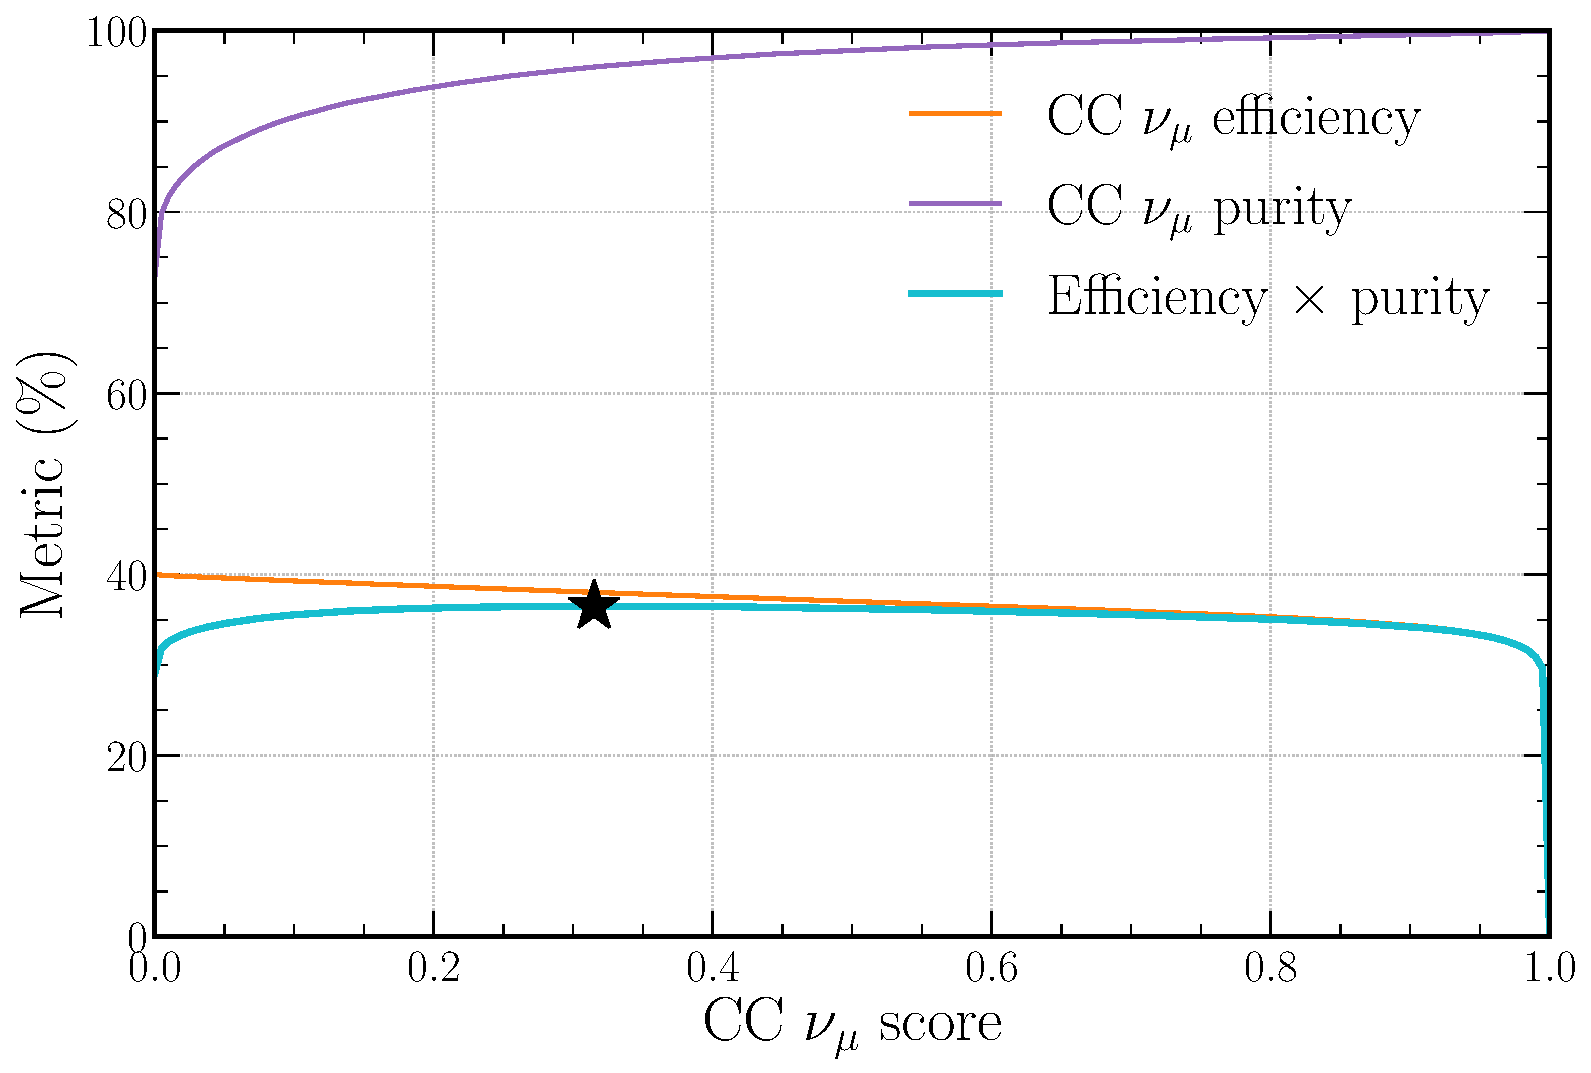
\includegraphics[width=0.7\textwidth]{diagrams/7-results/final_numu_eff_curves.pdf}
    \caption[CC $\nu_{\mu}$ efficiency, purity and $\mathrm{efficiency}\times\mathrm{purity}$]
    {CC $\nu_{\mu}$ efficiency, purity and $\mathrm{efficiency}\times\mathrm{purity}$ for
        different values of CC $\nu_{\mu}$ score selection.}
    \label{fig:final_numu_eff_curves}
\end{figure}

\begin{table}
    \begin{tabular}{cccccc}
                 & CC $\nu_{\mu}$ sig & App CC $\nu_{e}$ bkg & Beam CC $\nu_{e}$ bkg & NC bkg        & Sig Purity     \\
        \midrule
        Cuts Num & 818.0              & 40.8                 & 33.0                  & 231.0         & $72.9\pm0.5\%$ \\
        FOM Num  & 777.9              & 1.32                 & 1.37                  & 29.3          & $96.1\pm0.6\%$ \\
        \midrule
        FOM Eff  & $38.0\pm0.2\%$     & $3.0\pm0.1\%$        & $4.0\pm0.1\%$         & $8.4\pm0.2\%$ & -              \\
    \end{tabular}
    \caption[Table showing CC $\nu_{\mu}$ selected event numbers, efficiencies and signal purity.]
    {Table showing CC $\nu_{\mu}$ selected event numbers and corresponding efficiencies for the
        various event categories as well as the associated signal purity. Shown are the numbers
        for both the post preselection, \emph{cosmic score} cut, and \emph{escapes score} cut
        numbers (Cuts) in addition to the $\mathrm{efficiency}\times\mathrm{purity}$ optimised
        (FOM) selection for which the efficiency is shown.}
    \label{tab:numu_selection}
\end{table}

The $\mathrm{efficiency}\times\mathrm{purity}$ optimised CC $\nu_{\mu}$ selection efficiency as a
function of energy for the different event categories is shown in Fig.~\ref{fig:final_numu_hists}.
Survived CC $\nu_{\mu}$ selection efficiency peaks just below \unit{2}{\GeV} before slowly
declining, this is entirely explained by higher energy events being less likely to have their
primary charged muon fully contained within the detector. Of interest is the expected dip in the
otherwise very high (>90\%) CC $\nu_{\mu}$ purity at approximately \unit{1.5}{\GeV} corresponding
to the oscillation maximum as shown in Fig.~\ref{fig:osc_cp_probs}. As in the CC $\nu_{e}$
selection case the NC efficiency is seen to rise with energy, again likely due to
misidentification of energetic protons and pions.

\begin{figure} % FINAL NUMU HISTS DIAGRAM %
    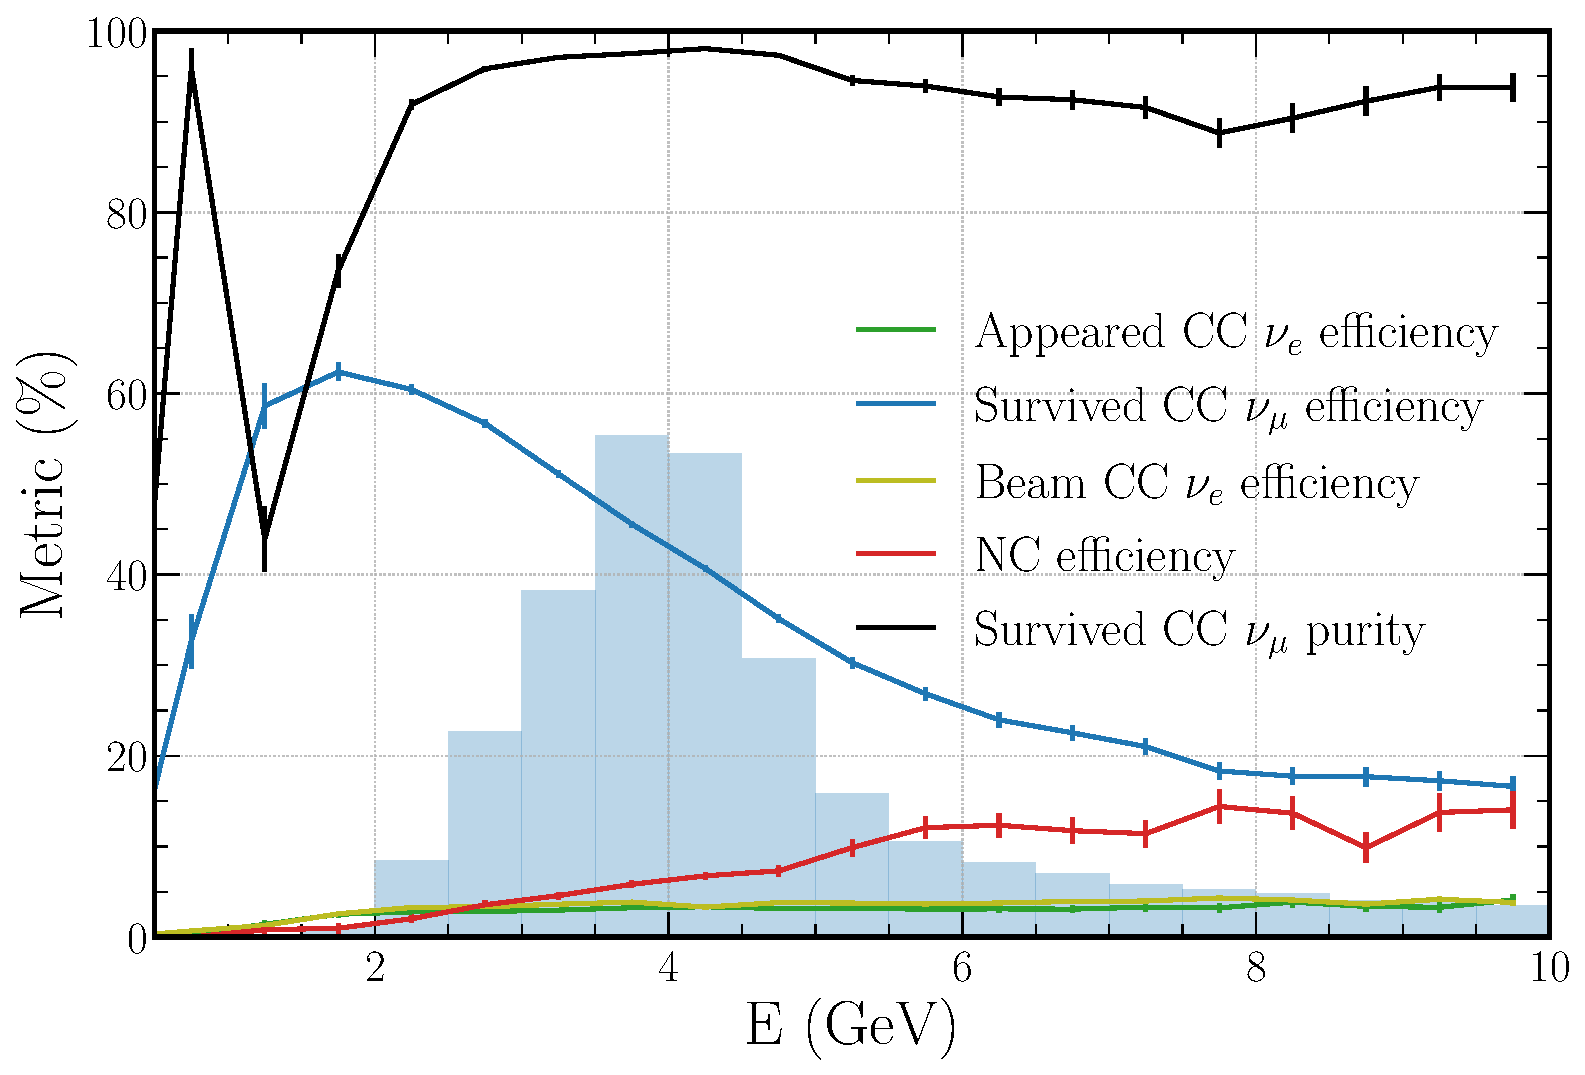
\includegraphics[width=0.7\textwidth]{diagrams/7-results/final_numu_hists.pdf}
    \caption[Efficiency of CC $\nu_{\mu}$ selection as a function of energy]
    {Efficiency of CC $\nu_{\mu}$ selection for the different event categories as well as survived
        CC $\nu_{\mu}$ purity as a function of neutrino energy. All CC categories are shown in terms
        of neutrino energy, while NC events are shown in terms of the hadronic component energy. For
        reference, the true survived CC $\nu_{\mu}$ neutrino energy distribution is shown in the
        blue.}
    \label{fig:final_numu_hists}
\end{figure}

\subsubsection*{Interaction type classification} %%%%%%%%%%%%%%%%%%%%%%%%%%%%%%%%%%%%%%%%%%%%%%%%%

Using the \emph{CC category} output of the trained beam classification network, the CC interaction
type (used in the following energy estimation section) for both CC $\nu_{e}$ and CC $\nu_{\mu}$
selected events can be determined. As in the \emph{combined category} output case, the
highest-scoring neuron can be used for classification, resulting in the matrix shown in
Fig.~\ref{fig:final_cc_cat_confusion}. Note that only events which are selected by either the CC
$\nu_{e}$ or CC $\nu_{\mu}$ selection are shown.

\begin{figure} % FINAL CC CAT CONFUSION DIAGRAM %
    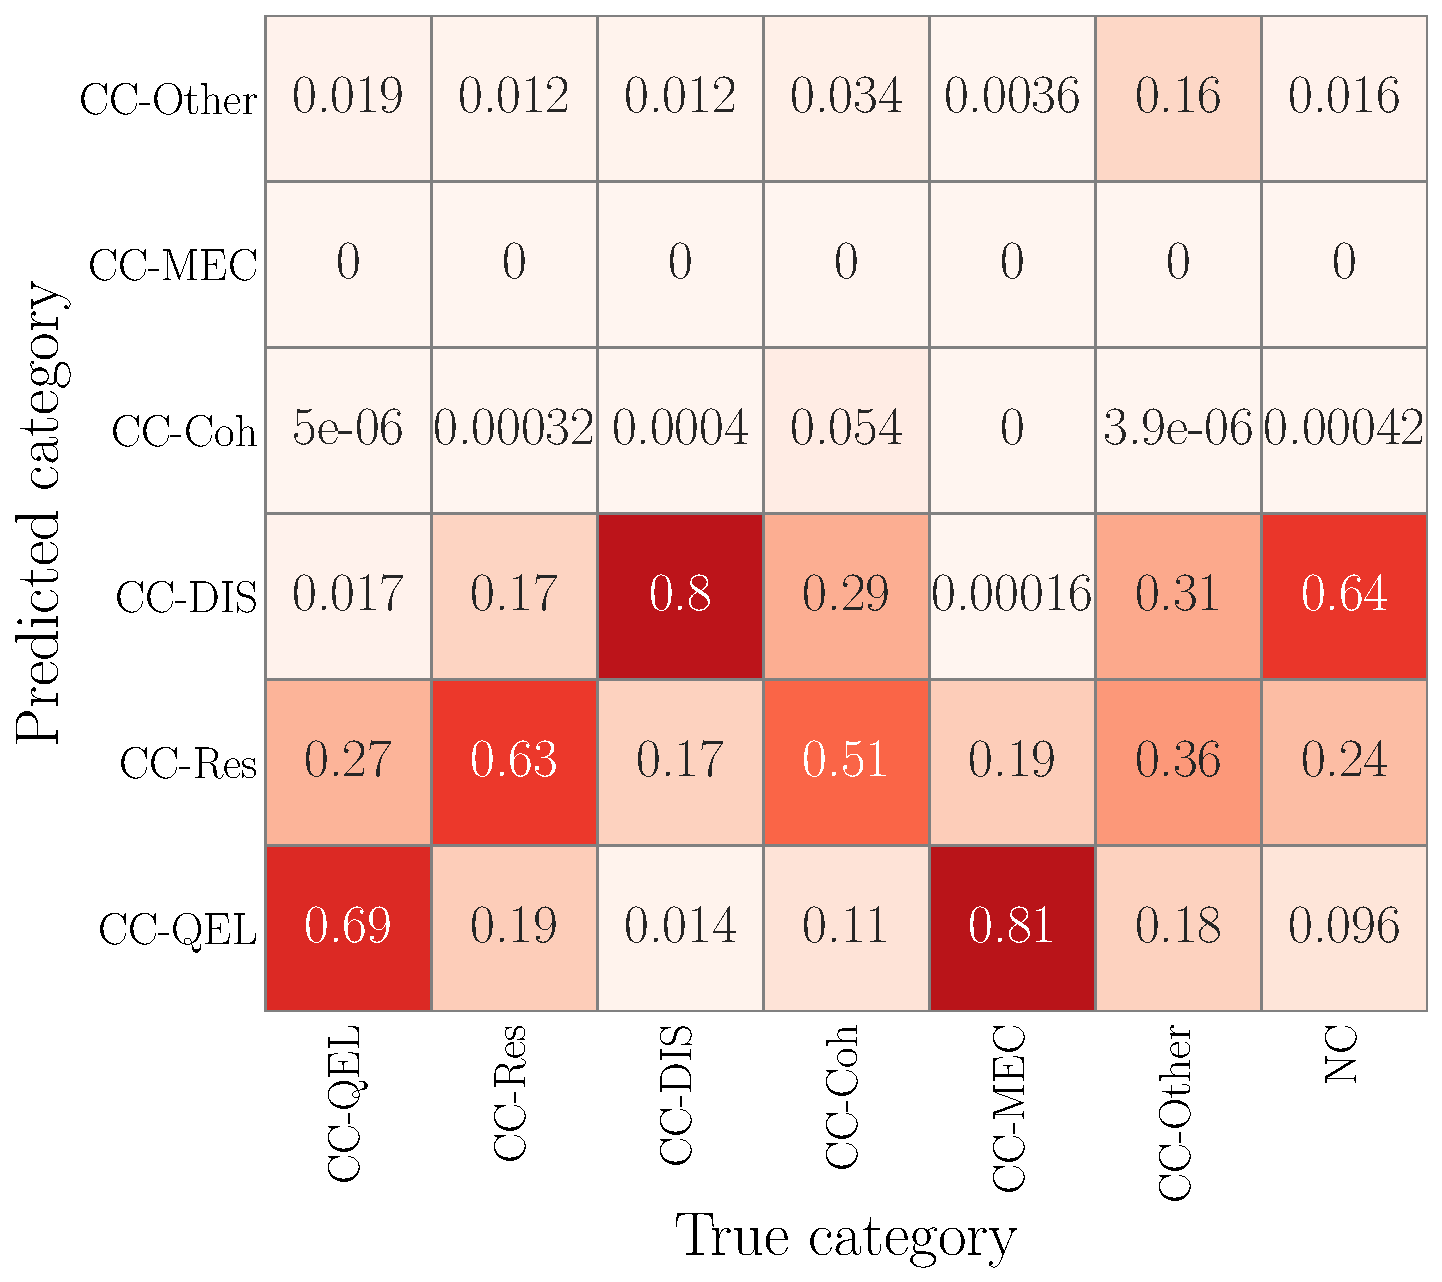
\includegraphics[width=0.7\textwidth]{diagrams/7-results/final_cc_cat_confusion.pdf}
    \caption[Classification matrix for the CC category output of the beam classification network]
    {Classification matrix for the \emph{CC category} output of the trained beam classification
        network. Shown are events that have either been selected by the CC $\nu_{e}$ or CC
        $\nu_{\mu}$ selection. Events are simply classified using the categorical score for which
        they have the highest value. The numbers shown are the fraction of true category events
        classified into each of the six possible categories.}
    \label{fig:final_cc_cat_confusion}
\end{figure}

Reasonable classification accuracy greater than 60\% is achieved across the three dominant
interaction types CC-QEL, CC-Res, and CC-DIS. The less common CC-Coh and CC-MEC types are found to
be commonly misidentified as CC-Res and CC-QEL respectively, likely due to the imbalanced training
dataset and their corresponding topological similarities. Background NC events which pass either
CC $\nu_{e}$ or CC $\nu_{\mu}$ selection (commonly high in energy) are found to be typically
classified as CC-DIS in nature; this is expected as they commonly contain multiple visible
particles in the final state as do CC-DIS events.

For completeness, the \emph{NC category} classification matrix is shown in
Fig.~\ref{fig:final_nc_cat_confusion} for events that are neither classified as CC $\nu_{e}$ or CC
$\nu_{\mu}$. As in the CC case, the dominant interaction types NC-Res and NC-DIS are classified
well, with NC-Coh events typically being classified as NC-Res. Of the CC events that are not
selected, the vast majority are classified as NC-DIS events. Similarly to above, this is likely
due to multiple energetic particles in the final state, for which the beam classification network
determined no clear charged lepton.

\begin{figure} % FINAL NC CAT CONFUSION DIAGRAM %
    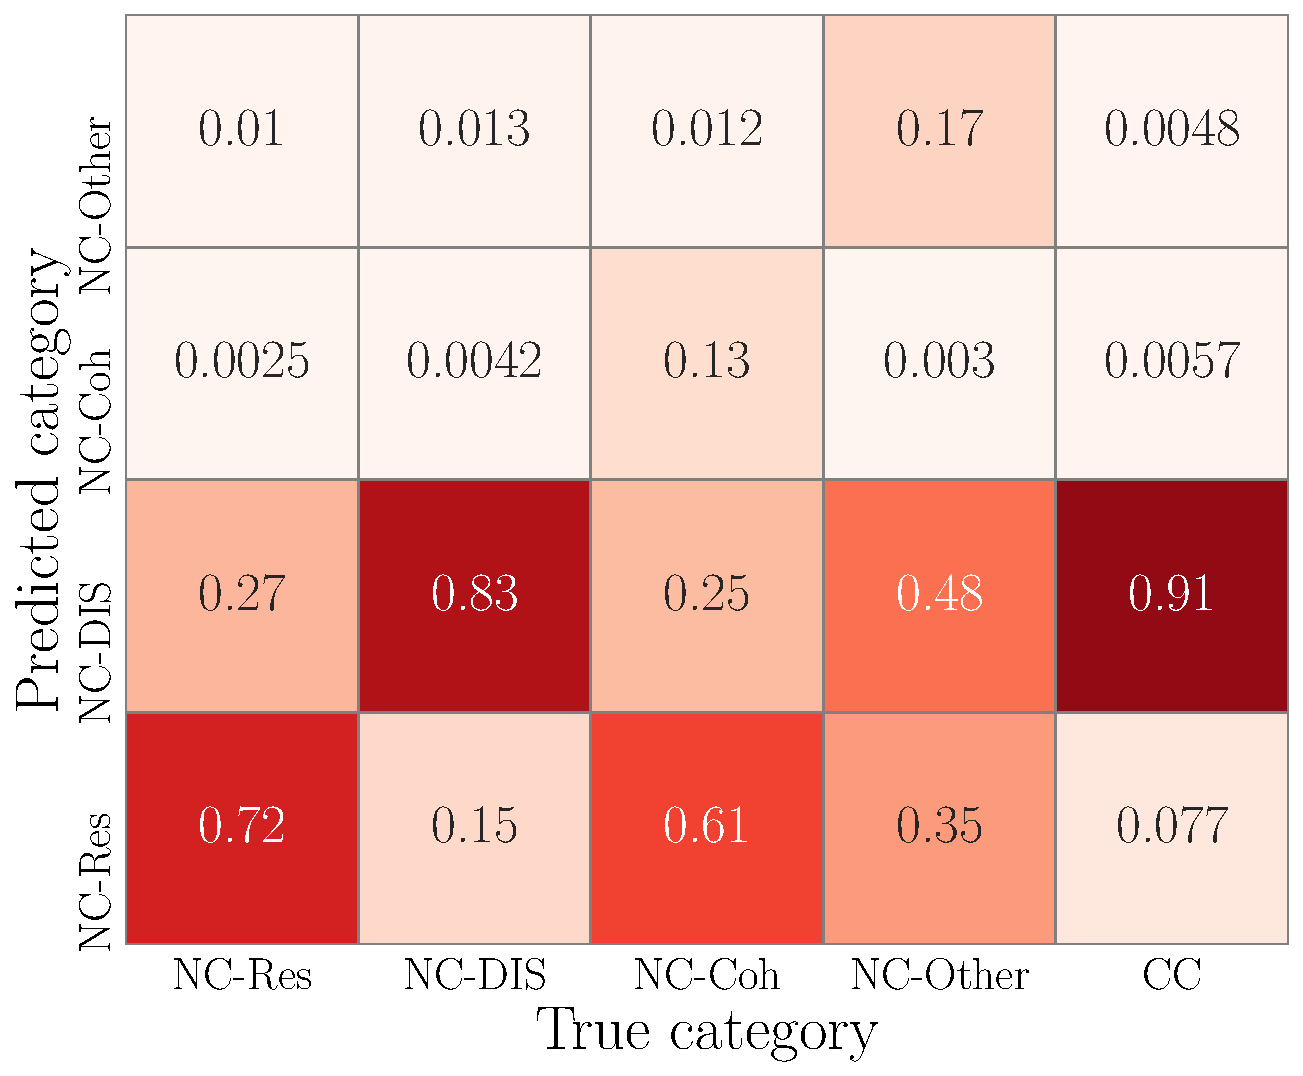
\includegraphics[width=0.7\textwidth]{diagrams/7-results/final_nc_cat_confusion.pdf}
    \caption[Classification matrix for the NC category output of the beam classification network]
    {Classification matrix for the \emph{NC category} output of the trained beam classification
        network. Events are simply classified using the categorical score for which they have the
        highest value. The numbers shown are the fraction of true category events classified into
        each of the four possible categories.}
    \label{fig:final_nc_cat_confusion}
\end{figure}

\subsection{Energy and vertex estimation} %%%%%%%%%%%%%%%%%%%%%%%%%%%%%%%%%%%%%%%%%%%%%%%%%%%%%%%%
\label{sec:results_eval_energy} %%%%%%%%%%%%%%%%%%%%%%%%%%%%%%%%%%%%%%%%%%%%%%%%%%%%%%%%%%%%%%%%%%

By using the CC interaction type classification just presented, the differences between CC
interaction types can be exploited to improve neutrino energy, charged lepton energy, and
interaction vertex position and time estimation. For events classified as either CC $\nu_{e}$ or
CC $\nu_{\mu}$ with an associated \emph{CC category} interaction type, the corresponding bespoke
trained network outlined in Section.~\ref{sec:cnn_specific_energy} is used.

Only three networks for each neutrino type are trained, one for each of the dominant interaction
types CC-QEL(CC-MEC), CC-Res, or CC-DIS. For events not classified by \emph{CC category} as one of
these categories, such as CC-Coh or CC-Other, the CC-Res network is used as it is the most
topologically similar interaction type.

The distributions of CNN estimated (\emph{neutrino energy} output) and true $\nu_{e}$ and
$\nu_{\mu}$ neutrino energies for true CC $\nu_{e}$ and CC $\nu_{\mu}$ events respectively that
are also selected by their corresponding CC selection are shown in
Fig.~\ref{fig:final_energy_dists}. The CNN estimated distributions match the truth well across the
full range of neutrino energies expected within \chipsfive, except perhaps in the peak regions
where the exact truth distribution shape is not fully captured.

\begin{figure} % FINAL ENERGY DISTS DIAGRAM %
    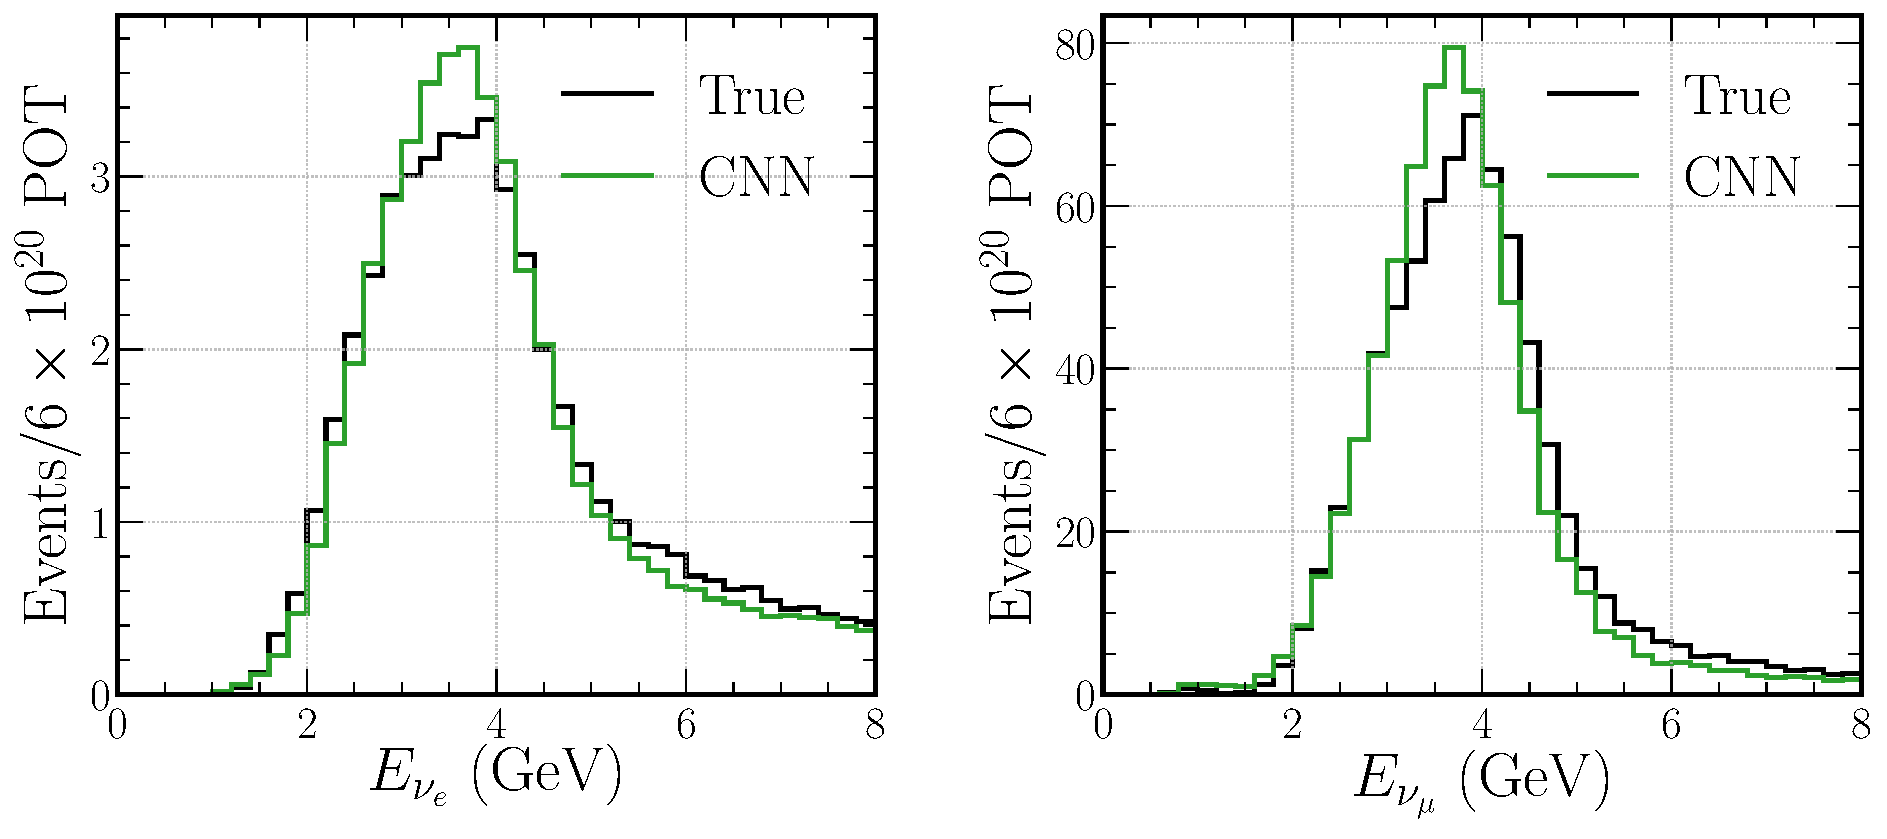
\includegraphics[width=0.8\textwidth]{diagrams/7-results/final_energy_dists.pdf}
    \caption[Distributions of true and CNN estimated neutrino energy]
    {Distributions of true and CNN estimated neutrino energy for CC $\nu_{e}$ (left) and CC
        $\nu_{\mu}$ (right) beam events. Only true CC $\nu_{e}$ and CC $\nu_{\mu}$ events that are
        also selected by the CC $\nu_{e}$ and CC $\nu_{\mu}$ selections respectively are shown.}
    \label{fig:final_energy_dists}
\end{figure}

As the training samples contain a spectrum of events typical of the beam, it is important to check
that the CNN neutrino energy estimation is not simply predicting an energy close to the expected
peak beam energy. The probability of a CNN estimated neutrino energy given a true neutrino energy
is shown in Fig.~\ref{fig:final_energy_2d} for both CC $\nu_{e}$ and CC $\nu_{\mu}$ events. CNN
estimated energy is found to be roughly equivalent to true energy across the full range of
expected \chipsfive beam energies, proving the desired trained network response.

\begin{figure} % FINAL 2D ENERGY DIAGRAM %
    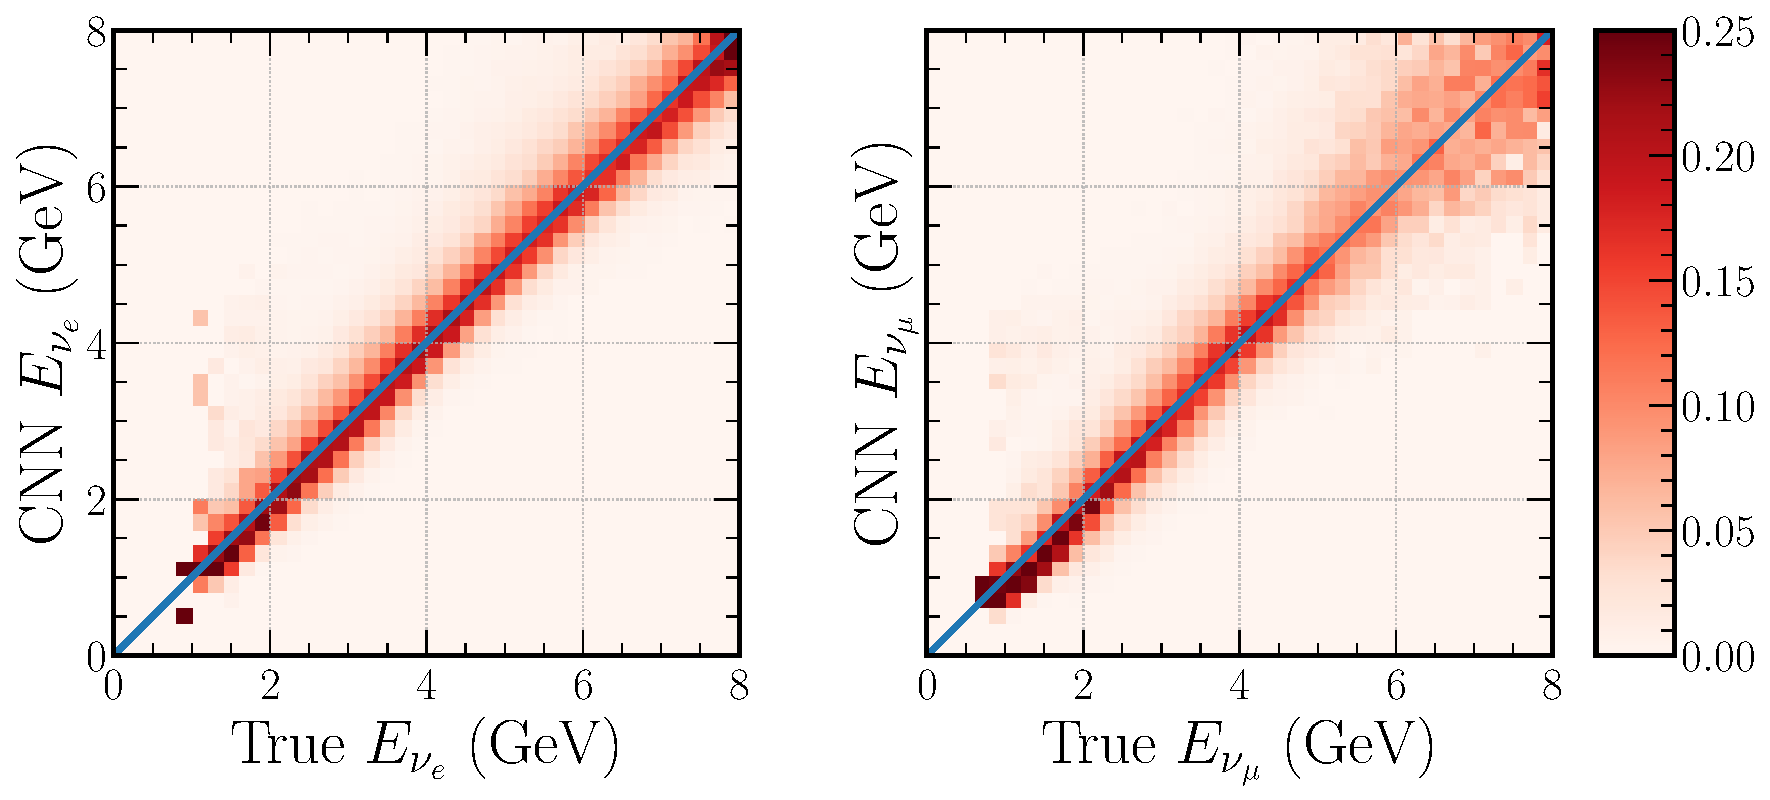
\includegraphics[width=0.8\textwidth]{diagrams/7-results/final_energy_2d.pdf}
    \caption[Probability of CNN estimated neutrino energy given a true neutrino energy]
    {Probability of CNN estimated neutrino energy given a true neutrino energy for CC $\nu_{e}$
        (left) and CC $\nu_{\mu}$ (right) beam events, with their equality shown in blue. Only
        true CC $\nu_{e}$ and CC $\nu_{\mu}$ events that are also selected by the CC $\nu_{e}$ and
        CC $\nu_{\mu}$ selections respectively are shown.}
    \label{fig:final_energy_2d}
\end{figure}

To fully understand CNN energy estimation performance, histograms of ratios of differences between
CNN estimated (reco) and true neutrino energy to true neutrino energy for both CC $\nu_{e}$ and CC
$\nu_{\mu}$ beam events are shown in Fig.~\ref{fig:final_energy_frac}. Distributions are shown for
both \emph{all} selected events and just the true \emph{signal} component within the corresponding
beam selection. Similar distributions splitting the \emph{signal} component by interaction type
are shown in Fig.~\ref{fig:final_energy_frac_split}. Furthermore, a summary of the neutrino energy
resolutions achieved for both CC $\nu_{e}$ and CC $\nu_{\mu}$ events is shown in
Tab.~\ref{tab:energy_resolutions}.

\begin{figure} % FINAL ENERGY FRAC DIAGRAM %
    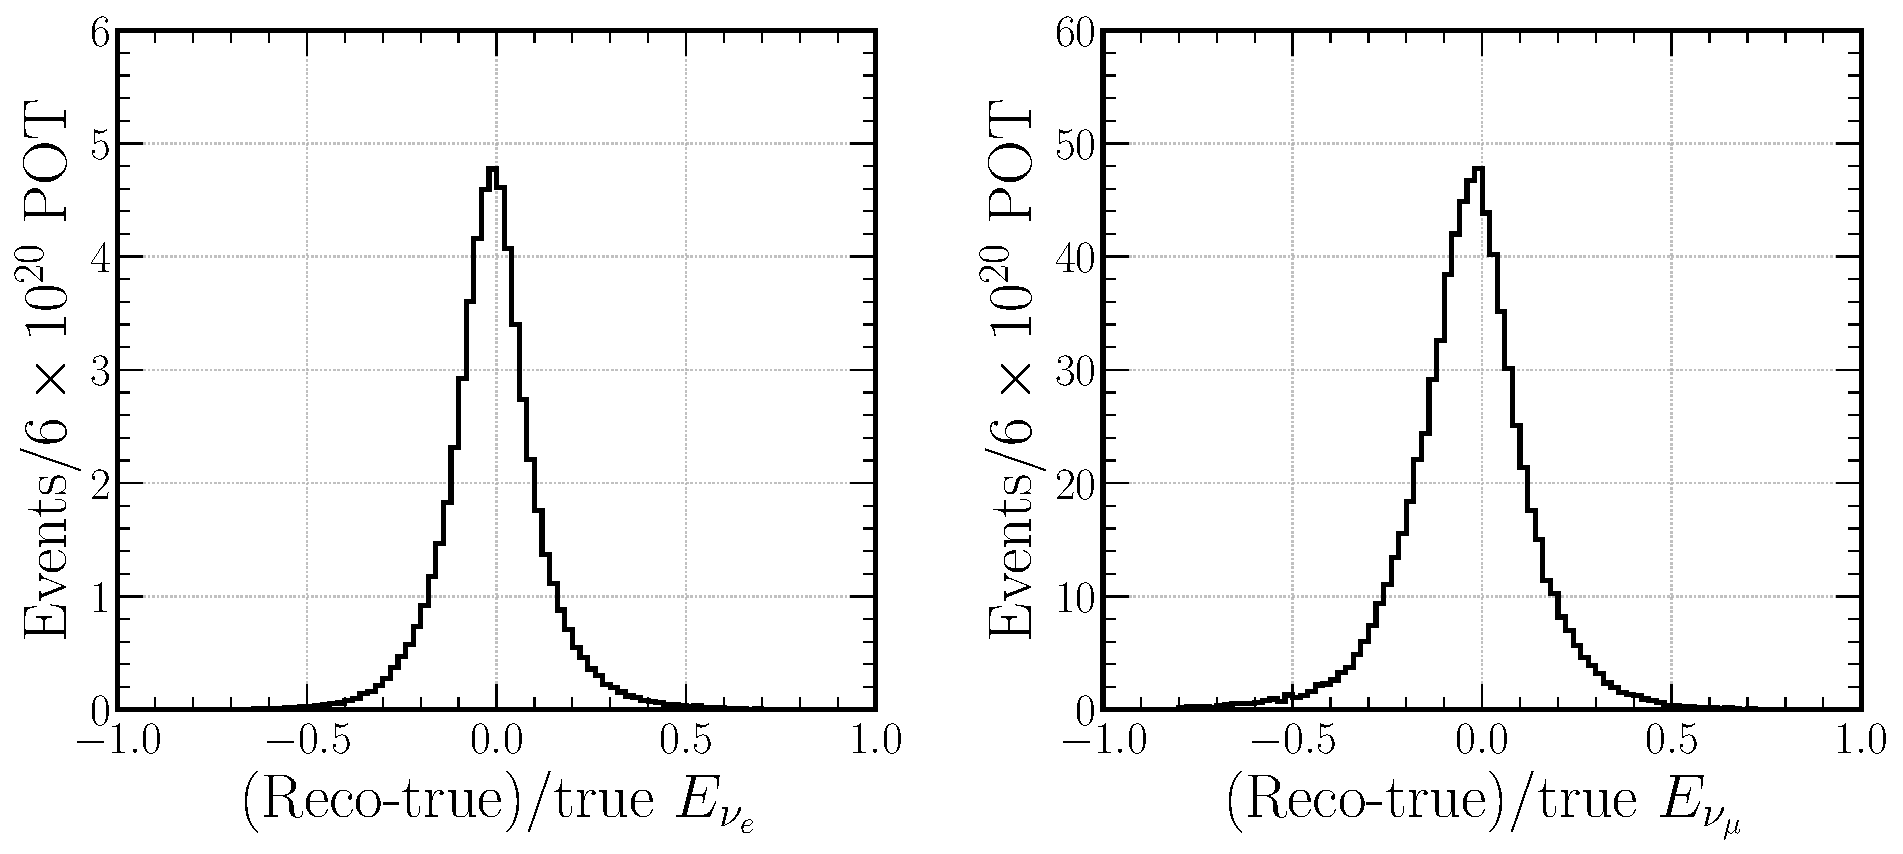
\includegraphics[width=0.8\textwidth]{diagrams/7-results/final_energy_frac.pdf}
    \caption[Distributions of (reco-true)/true neutrino energies]
    {Distributions of (reco-true)/true neutrino energies for both CC $\nu_{e}$ (left) and CC
        $\nu_{\mu}$ (right) beam events. Distributions for both \emph{all} respectively selected
        events and just the \emph{signal} component of each selection are shown.}
    \label{fig:final_energy_frac}
\end{figure}

\begin{figure} % FINAL ENERGY FRAC SPLIT DIAGRAM %
    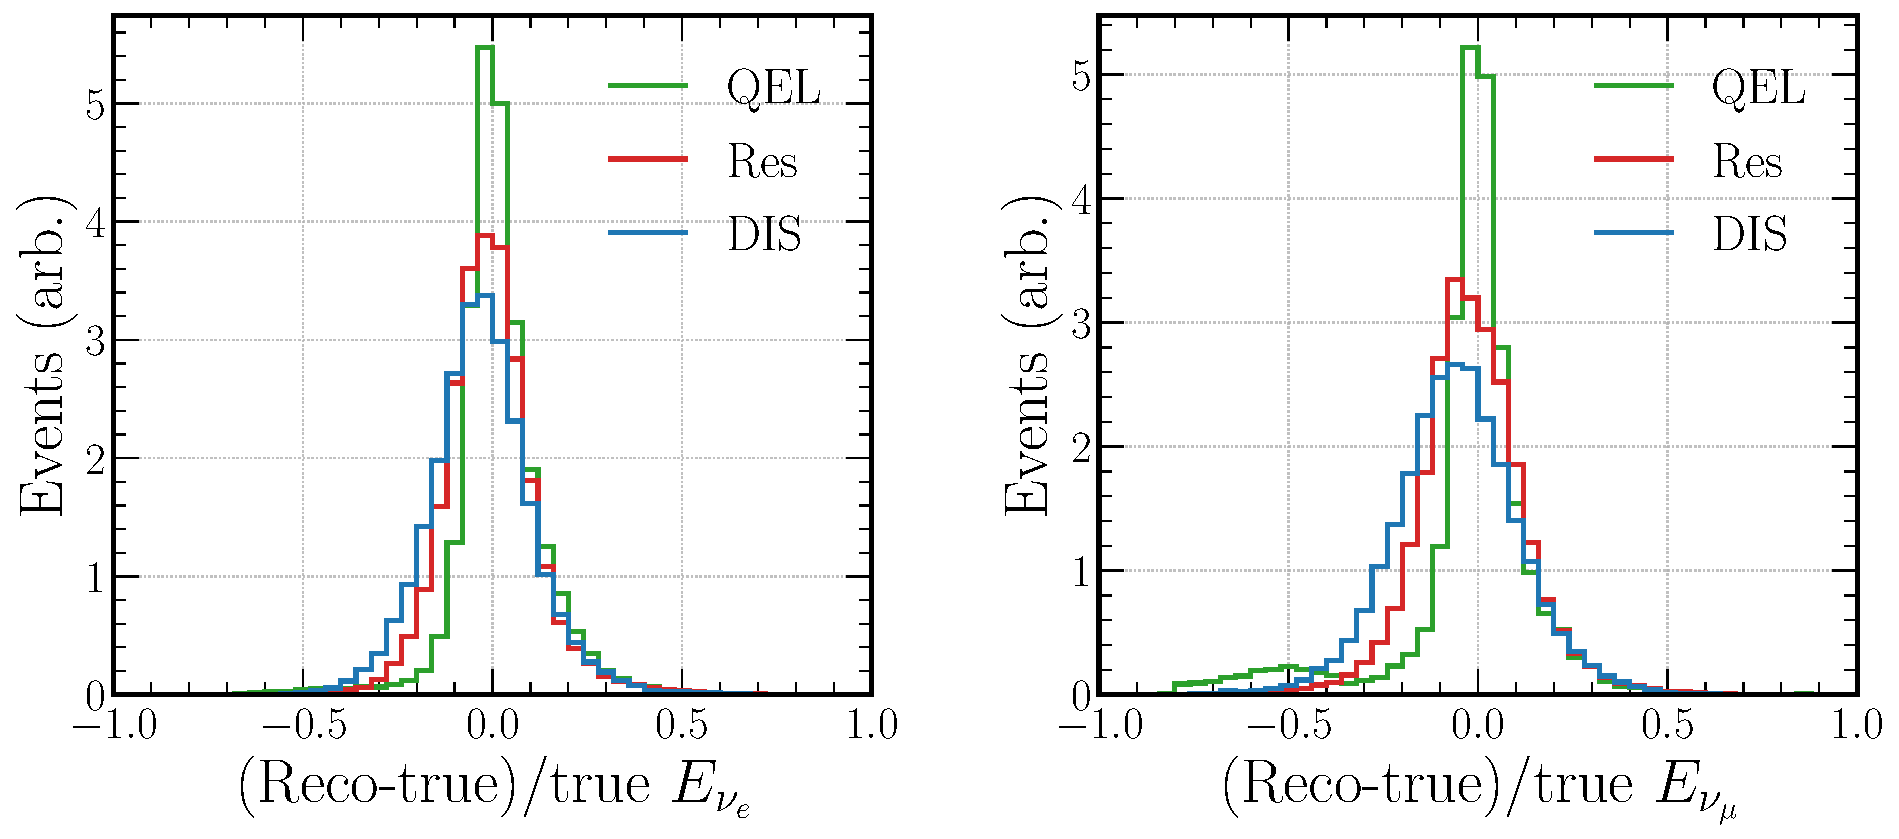
\includegraphics[width=0.8\textwidth]{diagrams/7-results/final_energy_frac_split.pdf}
    \caption[Distributions of (reco-true)/true neutrino energies by interaction type]
    {Distributions of (reco-true)/true neutrino energies for both CC $\nu_{e}$ (left) and CC
        $\nu_{\mu}$ (right) signal beam events by interaction types. The relative number of events
        between interaction types has been scaled for clearer comparison.}
    \label{fig:final_energy_frac_split}
\end{figure}

\begin{table}
    \begin{tabular}{lccccc}
        Event type     & All    & Signal & Signal-QEL & Signal-Res & Signal-DIS \\
        \midrule
        CC $\nu_{e}$   & 12.9\% & 10.3\% & 7.1\%      & 10.3\%     & 13.6\%     \\
        CC $\nu_{\mu}$ & 12.9\% & 12.6\% & 6.2\%      & 11.7\%     & 14.9\%     \\
    \end{tabular}
    \caption[Summary of CC $\nu_{e}$ and CC $\nu_{\mu}$ neutrino energy resolutions]
    {Summary of CC $\nu_{e}$ and CC $\nu_{\mu}$ neutrino energy resolutions. Shown for each sample
        are the resolutions for \emph{all} selected events, the true \emph{signal} selected events
        and the three dominant \emph{signal} interaction type components, QEL, Res, and DIS. The
        resolutions are calculated from the standard deviations of gaussian fits made to the
        distributions shown in Fig.~\ref{fig:final_energy_frac} and
        Fig.~\ref{fig:final_energy_frac_split}.}
    \label{tab:energy_resolutions}
\end{table}

The tail of negative values for the \emph{all} selected CC $\nu_{e}$ distribution in
Fig.~\ref{fig:final_energy_frac} indicates that wrongly classified CC $\nu_{e}$ events, mainly NC
in nature, are typically estimated with neutrino energy lower than their actual value. This is
expected given the missing energy of the final state neutrino. Additionally, the interaction type
resolutions follow the expected pattern, with simple to reconstruct single charged lepton QEL
interactions achieving an improved resolution compared to multi-particle DIS events. Furthermore,
these results are very similar to the selected signal energy resolutions obtained by \nova of
10.7\% for CC $\nu_{e}$ events and 9.1\% for CC $\nu_{\mu}$ events~\cite{acero2019}.

By making gaussian fits to the (reco-true)/true signal neutrino energy distributions shown in
Fig.~\ref{fig:final_energy_frac} in \unit{1}{GeV} wide true neutrino energy bins, how the
resolution changes with energy can be explored. The means and standard deviations of these fits
are shown in Fig.~\ref{fig:final_energy_nuel} and Fig.~\ref{fig:final_energy_numu} for CC
$\nu_{e}$ and CC $\nu_{\mu}$ events respectively, split by interaction type.

Reasonably significant bias in the means is observed with respect to the true neutrino energy for
both $\nu_{e}$ and CC $\nu_{\mu}$ events. This is particularly true of DIS events, but still
significant for Res and QEL events. As a (peaked) flux distribution of events is used for training
as opposed to a flat flux, this is expected. As a consequence, any future energy estimation work
should consider the flat flux approach, as explored in Ref.~\cite{baldi2019}. The standard
deviation is seen to decrease with true neutrino energy for all interaction types, except for
energies above the main flux peak. Again, this is most likely due to the spectrum of events in the
training sample. A contributing factor, however, will be due to the inability of PMTs to
distinguish between numbers of incident photons at higher counts, more likely at higher energies.

\begin{figure} % FINAL NUEL ENERGY DIAGRAM %
    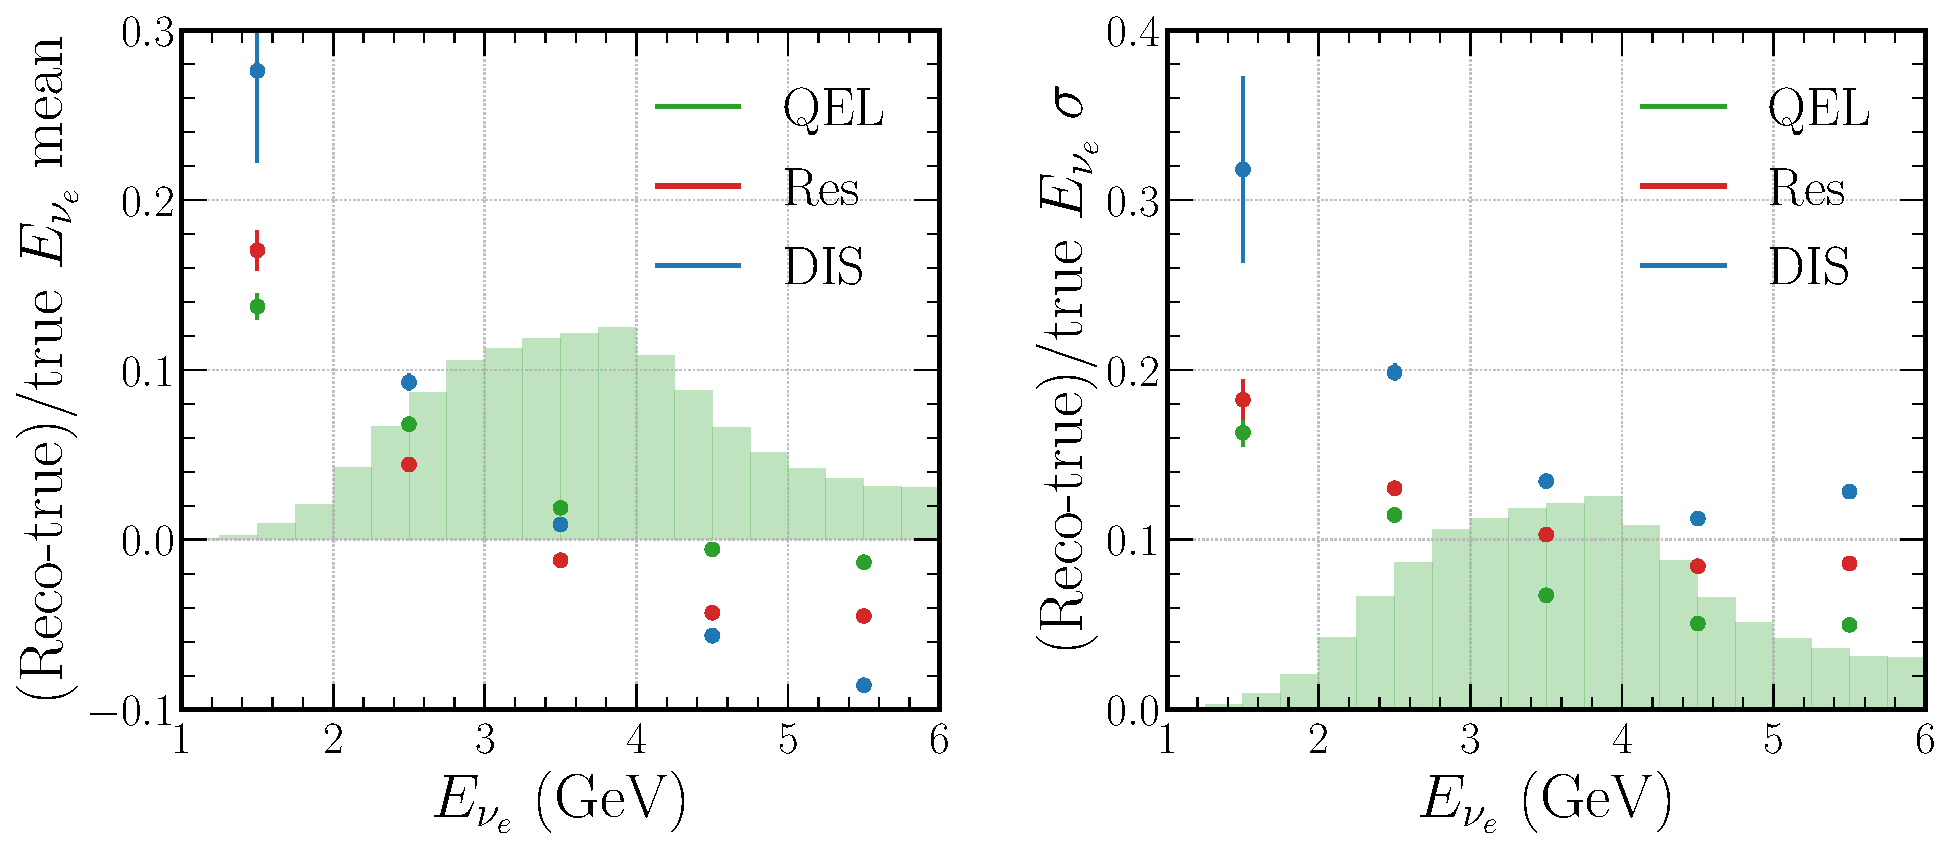
\includegraphics[width=\textwidth]{diagrams/7-results/final_energy_nuel.pdf}
    \caption[Means and standard deviations of fits to $\nu_{e}$ energy distributions]
    {Means (left) and standard deviations (right) of fits made to distributions of
        (reco-true)/true neutrino energy for CC $\nu_{e}$ events across a range of \unit{1}{GeV}
        wide true neutrino energy bins and split by interaction type. The true distribution of CC
        $\nu_{e}$ events is shown in green.}
    \label{fig:final_energy_nuel}
\end{figure}

\begin{figure} % FINAL NUMU ENERGY DIAGRAM %
    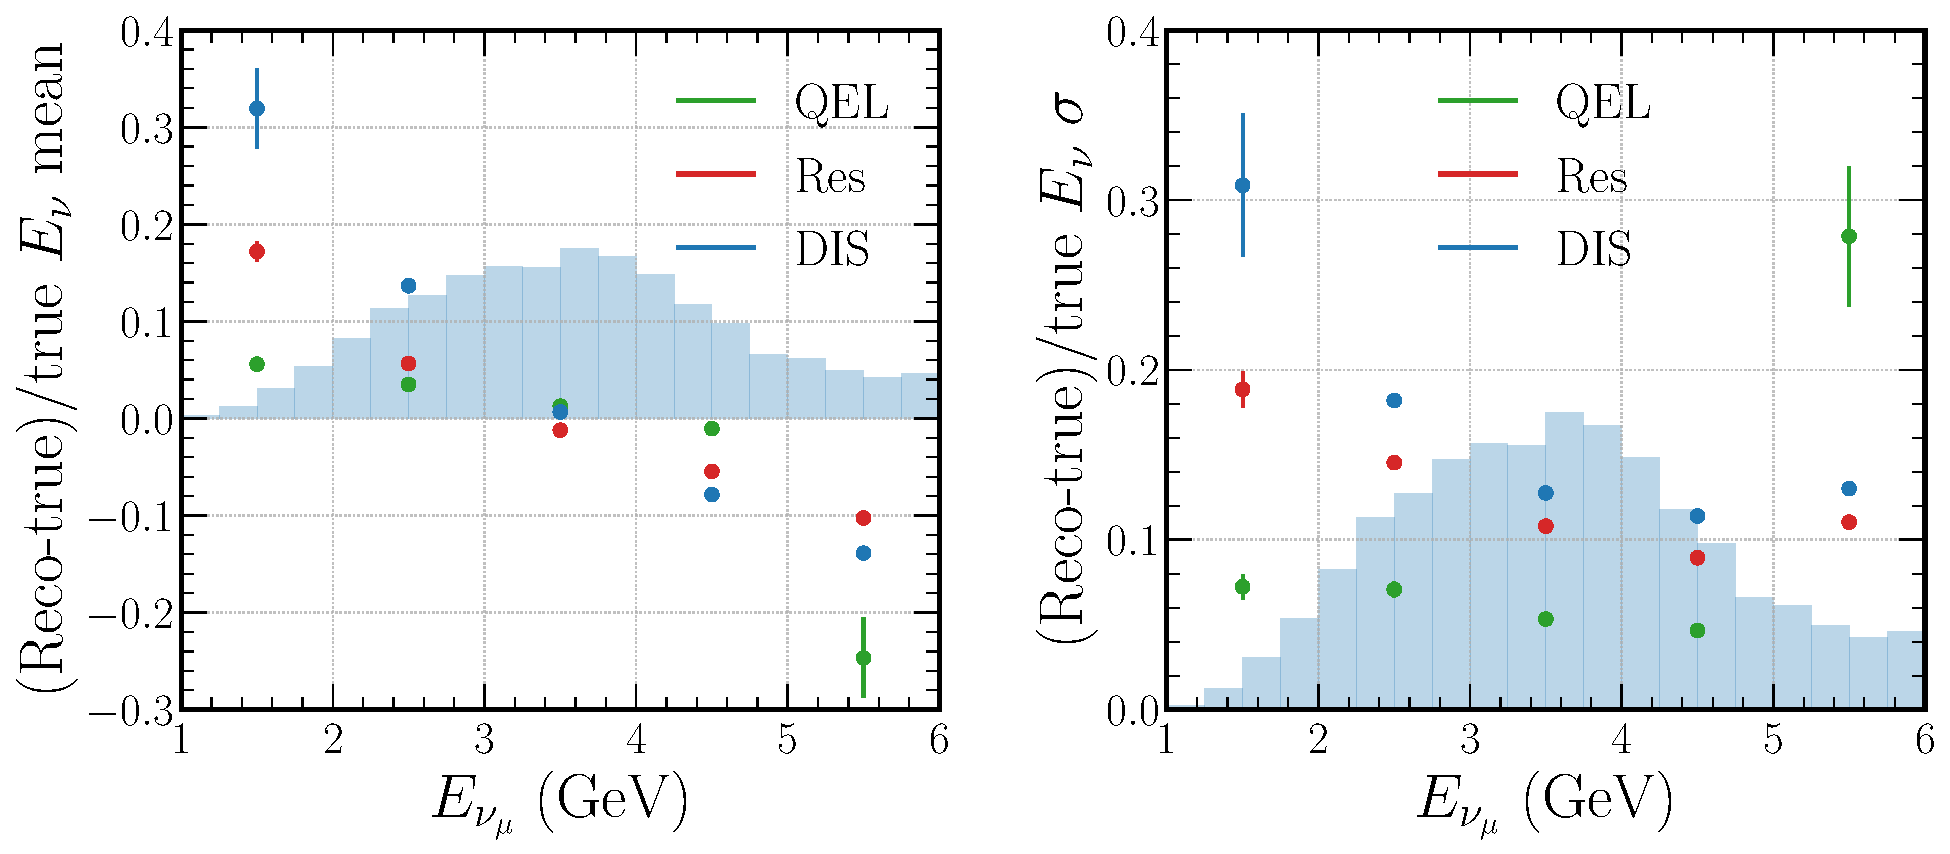
\includegraphics[width=\textwidth]{diagrams/7-results/final_energy_numu.pdf}
    \caption[Means and standard deviations of fits to $\nu_{\mu}$ energy distributions]
    {Means (left) and standard deviations (right) of fits made to distributions of
        (reco-true)/true neutrino energy for CC $\nu_{\mu}$ events across a range of \unit{1}{GeV}
        wide true neutrino energy bins and split by interaction type. The true distribution of CC
        $\nu_{\mu}$ events is shown in blue.}
    \label{fig:final_energy_numu}
\end{figure}

As in the CC $\nu_{e}$ selection case the best way to understand the relative performance of the
energy estimation is by comparison with the standard reconstruction presented in
Section.~\ref{sec:cnn_old_reco}. Although the standard reconstruction does not attempt to estimate
the neutrino energy, the energy of the primary charged lepton in each CC event is predicted, which
can be compared to the \emph{charged lepton energy} output of the energy estimation networks.
Histograms of ratios of differences between CNN estimated (reco) and true charged lepton energy to
true charged lepton energy for both CC $\nu_{e}$ and CC $\nu_{\mu}$ beam QEL events are shown in
Fig.~\ref{fig:final_frac_e_comparison}.

A significant improvement is made using the new CNN approach. An energy resolution 32\%(40\%) the
size of the standard reconstruction resolution for CC $\nu_{e}$($\nu_{\mu}$) QEL events is
achieved, at 4.5\%(4.0\%). When compared to the approximately 2.5\% CC QEL charged lepton energy
resolution reached by the fiTQun algorithm for Super-Kamiokande~\cite{jiang2019}, the performance
presented here is impressive, given the significant differences in detector design.

\begin{figure} % FINAL FRAC E COMPARISON DIAGRAM %
    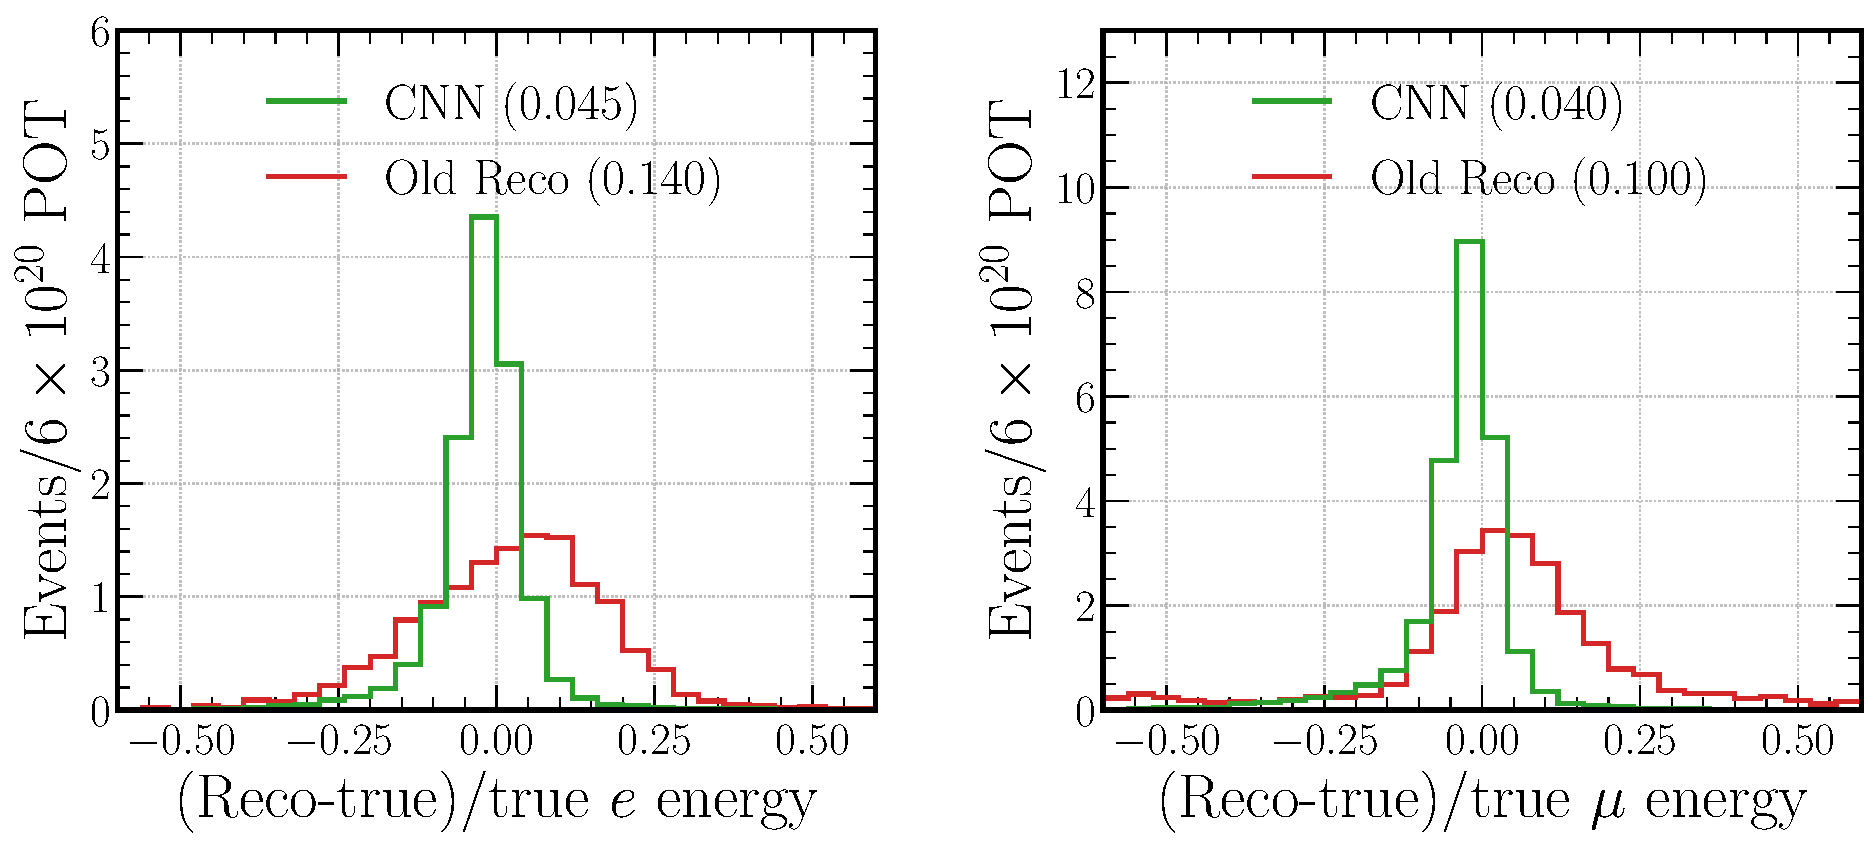
\includegraphics[width=0.8\textwidth]{diagrams/7-results/final_frac_e_comparison.pdf}
    \caption[Distributions of (reco-true)/true primary charged lepton energies for the CNN and standard methods]
    {Distributions of (reco-true)/true primary charged lepton energies for both CC $\nu_{e}$
        (left) and CC $\nu_{\mu}$ (right) beam events for both the new CNN approach and standard
        (old) methods. Only QEL events are shown for clearer comparison with the standard
        reconstruction methods. The standard deviation of a gaussian fit made to each distribution
        is shown in the corresponding brackets.}
    \label{fig:final_frac_e_comparison}
\end{figure}

The \emph{interaction vertex x-position}, \emph{interaction vertex y-position}, \emph{interaction
    vertex z-position}, and \emph{interaction time} outputs from the energy estimation networks can
also be used. Although not employed in this work, future analyses may require accurate fiducial
volume cuts or separation of events in time, therefore, strong performance is desirable. The CNN
estimated (reco) minus truth distributions are shown for selected signal CC $\nu_{e}$ and CC
$\nu_{\mu}$ QEL events in Fig.~\ref{fig:final_vertex_nuel_res_comparison} and
Fig.~\ref{fig:final_vertex_numu_res_comparison} respectively, with the standard reconstruction
method distributions additionally shown for comparison.

Comparable resolutions are achieved for CC $\nu_{e}$ events, while CC $\nu_{\mu}$ events display
considerable improvements in interaction vertex z-position and time. The Super-Kamiokande fiTQun
algorithm reaches an interaction vertex position resolution of \unit{20}{\mathrm{cm}} for CC
$\nu_{e}$ and \unit{15}{\mathrm{cm}} for CC $\nu_{\mu}$ events~\cite{jiang2019}, compared to the
approximately \unit{50}{\mathrm{cm}} and \unit{70}{\mathrm{cm}} resolutions in this work. Again, a
reasonable difference in performance, given the significant detector differences.

The charged lepton energy, interaction vertex position, and interaction vertex time resolutions
also display a clear advantage of the CNN approach. Long tails and mean biases are common in
distributions associated with the standard reconstruction when compared to the generally symmetric
distributions of the CNN approach. Commonly even more prevalent for non QEL events containing
multiple particles. This highlights how the multiple complex (human-influenced) inputs to the
standard reconstruction can both easily bias the outputs and not generalise well to all event
types.

\begin{figure} % FINAL VTX RES NUEL COMPARISON DIAGRAM %
    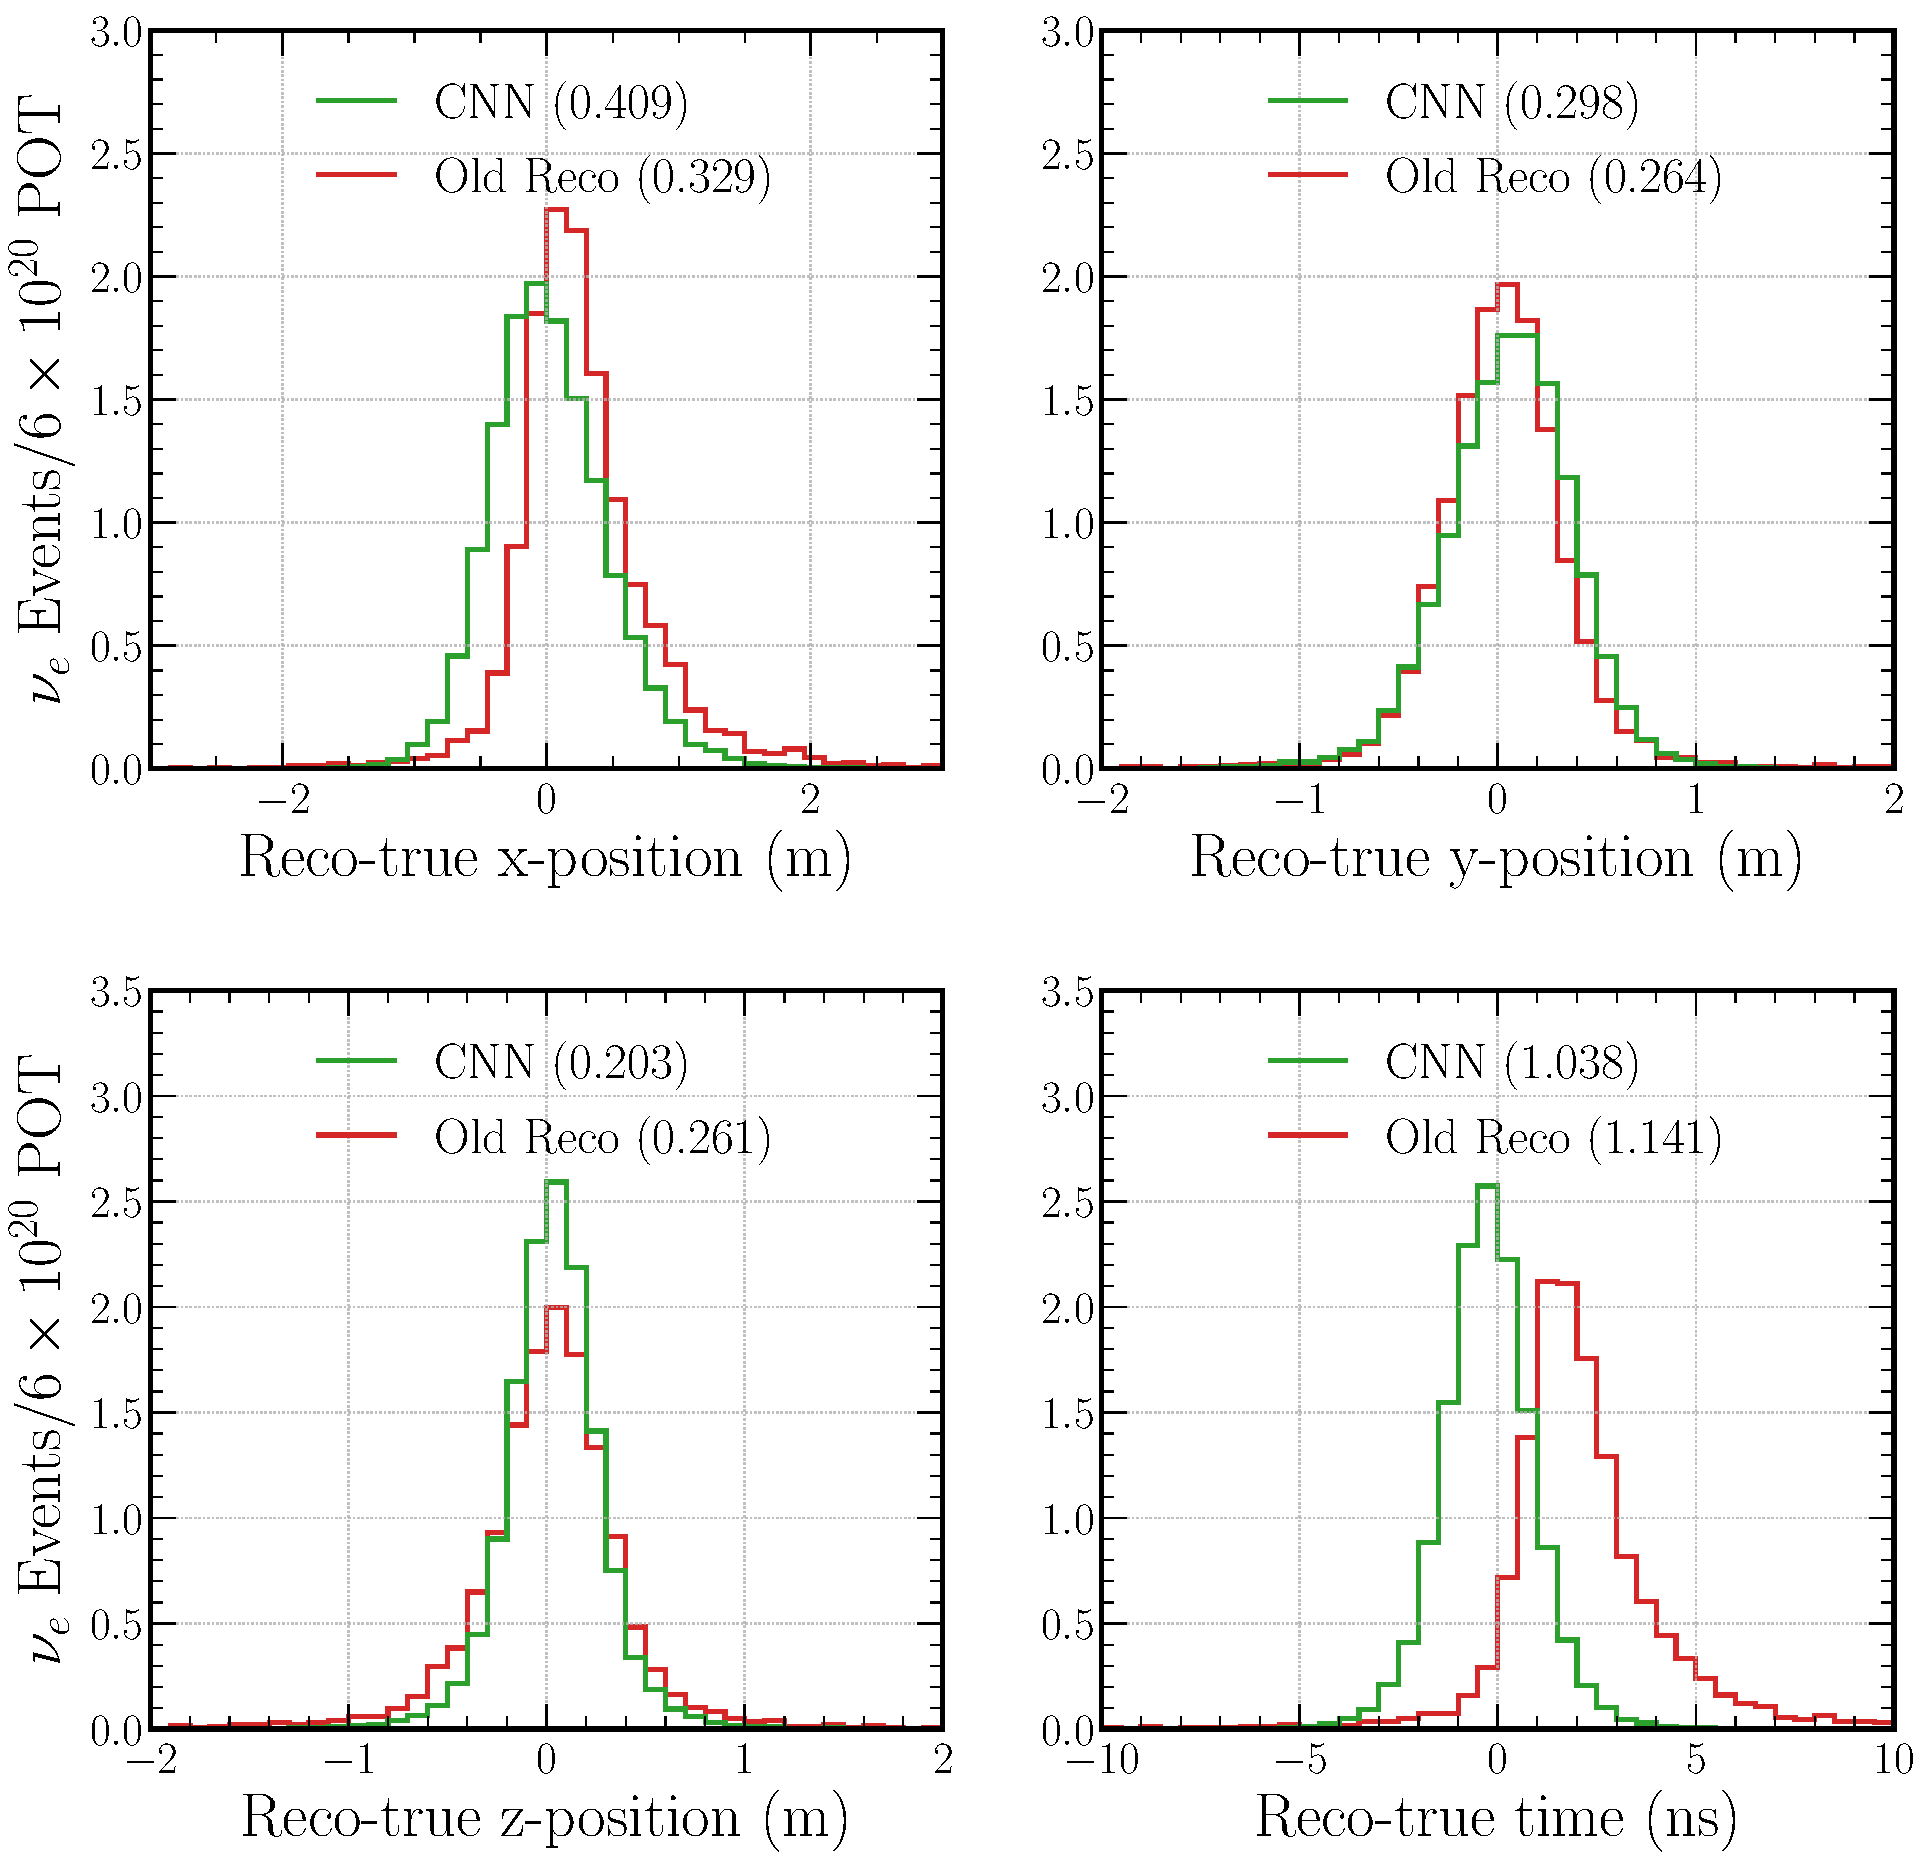
\includegraphics[width=0.8\textwidth]{diagrams/7-results/final_vertex_nuel_res_comparison.pdf}
    \caption[Reco-true distributions for the interaction vertex parameters for CC $\nu_{e}$ QEL
        events] {Reco-true distributions for the interaction vertex position components and time
        for CC $\nu_{e}$ QEL events. Both the distributions for the new CNN approach and standard
        (old) reconstruction methods are shown.}
    \label{fig:final_vertex_nuel_res_comparison}
\end{figure}

\begin{figure} % FINAL VTX RES NUMU COMPARISON DIAGRAM %
    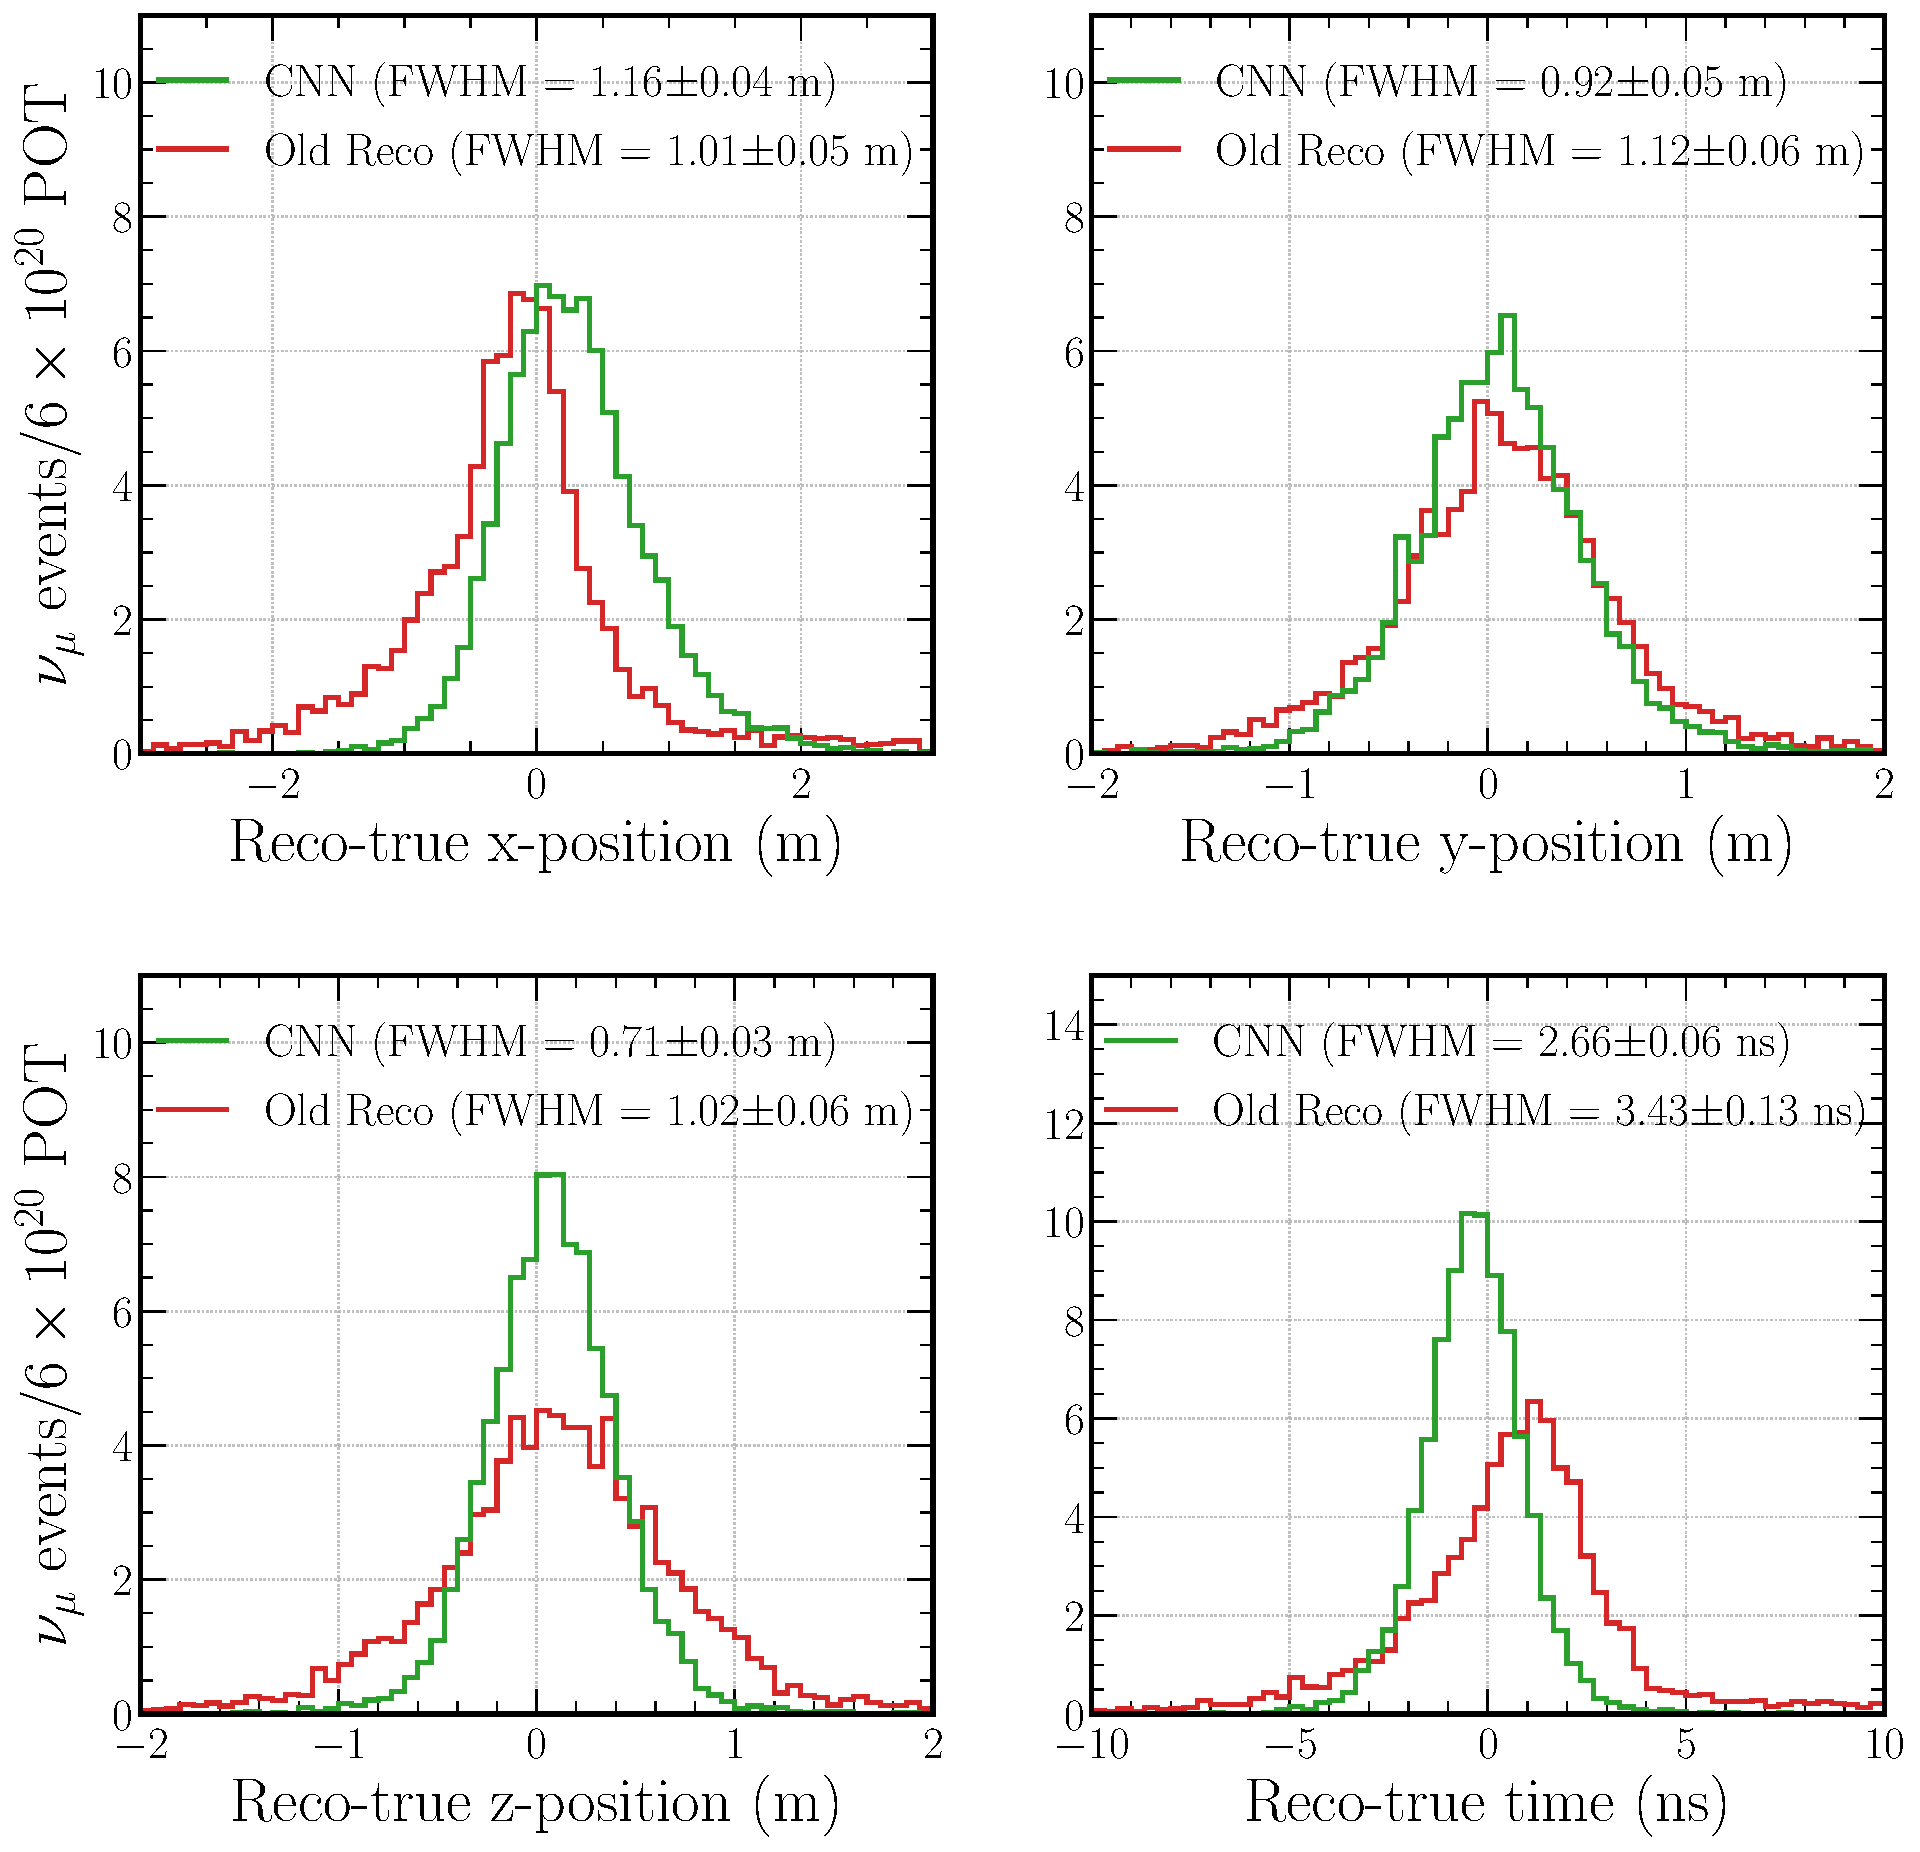
\includegraphics[width=0.8\textwidth]{diagrams/7-results/final_vertex_numu_res_comparison.pdf}
    \caption[Reco-true distributions for the interaction vertex parameters for CC $\nu_{\mu}$ QEL
        events] {Reco-true distributions for the interaction vertex position components and time
        for CC $\nu_{\mu}$ QEL events. Both the distributions for the new CNN approach and
        standard (old) reconstruction methods are shown.}
    \label{fig:final_vertex_numu_res_comparison}
\end{figure}

\subsection{Combined performance} %%%%%%%%%%%%%%%%%%%%%%%%%%%%%%%%%%%%%%%%%%%%%%%%%%%%%%%%%%%%%%%%
\label{sec:results_eval_combined} %%%%%%%%%%%%%%%%%%%%%%%%%%%%%%%%%%%%%%%%%%%%%%%%%%%%%%%%%%%%%%%%

By combining CC $\nu_{e}$ and CC $\nu_{\mu}$ selections with energy estimation, the final selected
spectrum of events within \chipsfive running for a year can be estimated for both. These are shown
in Fig.~\ref{fig:final_nuel_passed_energy_dist} and Fig.~\ref{fig:final_numu_passed_energy_dist}
for CC $\nu_{e}$ and CC $\nu_{\mu}$ selections respectively. Although, a detailed \chipsfive
sensitivity analysis is not included in this work, the expected curves for different values of
$\delta_{CP}$ are shown in the CC $\nu_{e}$ case for interest.

\begin{figure} % FINAL NUEL ENERGY DIST DIAGRAM %
    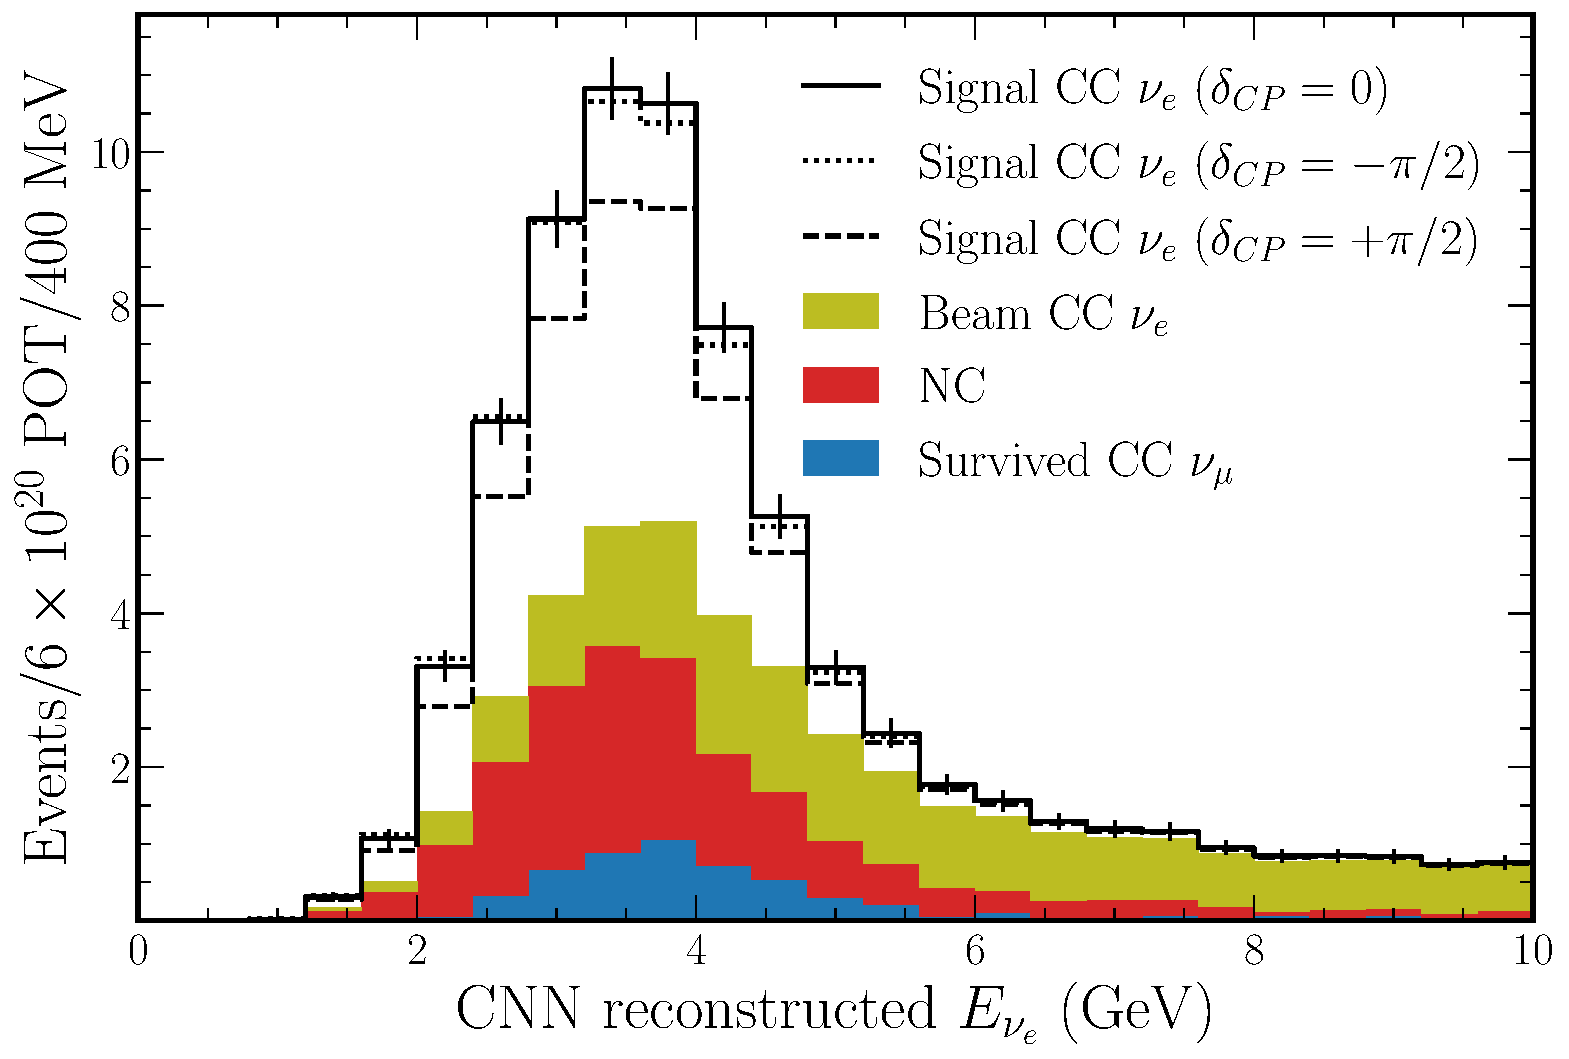
\includegraphics[width=0.8\textwidth]{diagrams/7-results/final_nuel_passed_energy_dist.pdf}
    \caption[Distribution of CNN reconstructed $\nu_{e}$ energies for CC $\nu_{e}$ selected events]
    {Distribution of CNN reconstructed $\nu_{e}$ energies for CC $\nu_{e}$ selected events. The
        appeared CC $\nu_{e}$ signal component as well as the intrinsic beam CC $\nu_{e}$, NC and
        survived CC $\nu_{\mu}$ background components are shown stacked to generate the full
        distribution. Expected totals are show in each bin for
        $\delta_{CP}=-\pi/2,~0,~\mathrm{and}~+\pi/2$.}
    \label{fig:final_nuel_passed_energy_dist}
\end{figure}

\begin{figure} % FINAL NUMU ENERGY DIST DIAGRAM %
    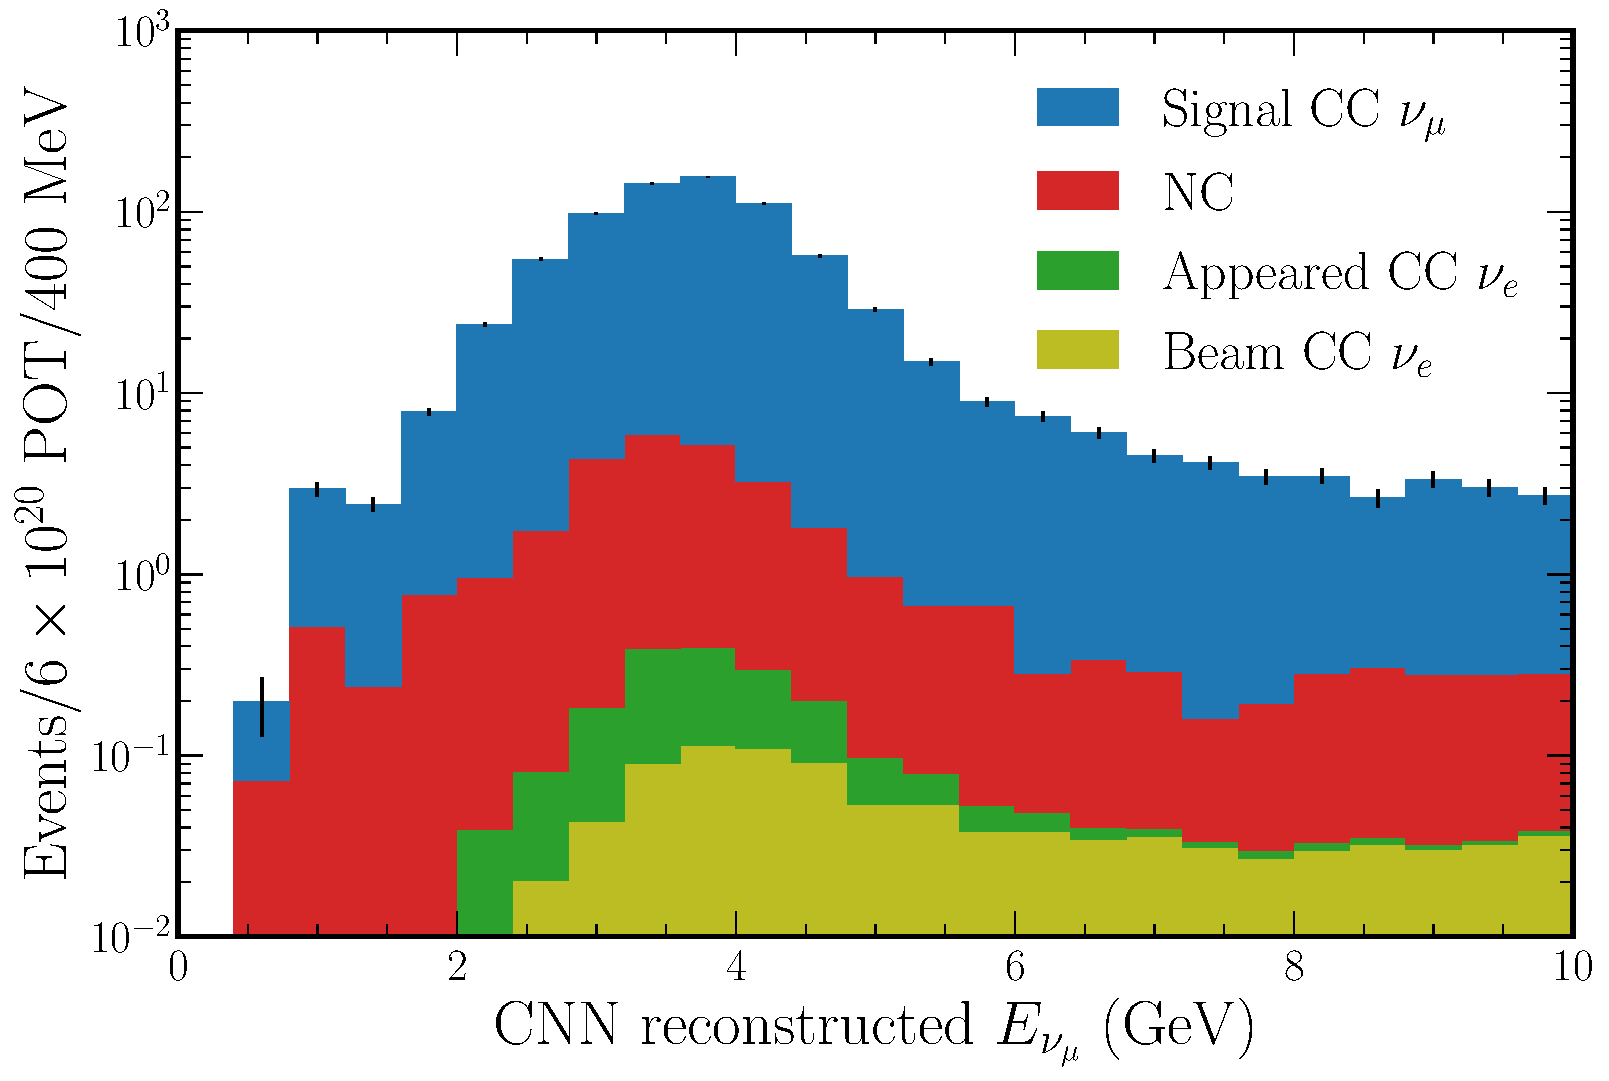
\includegraphics[width=0.8\textwidth]{diagrams/7-results/final_numu_passed_energy_dist.pdf}
    \caption[Distribution of CNN reconstructed $\nu_{\mu}$ energies for CC $\nu_{\mu}$ selected events]
    {Distribution of CNN reconstructed $\nu_{\mu}$ energies for CC $\nu_{\mu}$ selected events.
        The survived CC $\nu_{\mu}$ signal component as well as the appeared CC $\nu_{e}$,
        intrinsic beam CC $\nu_{e}$, and NC background components are shown stacked to generate
        the full distribution.}
    \label{fig:final_numu_passed_energy_dist}
\end{figure}

\section{Explainability} %%%%%%%%%%%%%%%%%%%%%%%%%%%%%%%%%%%%%%%%%%%%%%%%%%%%%%%%%%%%%%%%%%%%%%%%%
\label{sec:results_explain} %%%%%%%%%%%%%%%%%%%%%%%%%%%%%%%%%%%%%%%%%%%%%%%%%%%%%%%%%%%%%%%%%%%%%%

A common and justified concern with deep neural networks is their tendency to be used as a black
box (inputs in, outputs out) with no understanding of their inner working. For detailed physics
analyses, this can have significant implications for confidence in final results. Although
difficult quantitatively, qualitative assessments of the trained networks can go a long way to
proving they behave as desired. Here a sample of efforts to \emph{explain} the inner workings of
the trained CNNs presented in this work are described.

Visualisations of the output feature maps from the first, second, and third VGG blocks for each of
the trained networks (cosmic rejection, beam classification, and energy estimation) are shown in
Fig.~\ref{fig:cnn_visualisations} using the event shown in Fig.~\ref{fig:explain_example_event} as
input. Learnt Cherenkov ring features are observed, with different features activating different
feature maps differently. Ring edges, ring holes, outlying hits, Hough peaks, and a myriad of
combinations are observed proving each network learns features found to be important for its
outputs (tasks). Additionally, there are clear differences between the networks, with different
ring features proving important for different tasks.

\begin{figure} % EXPLAIN EXAMPLE EVENT DIAGRAM %
    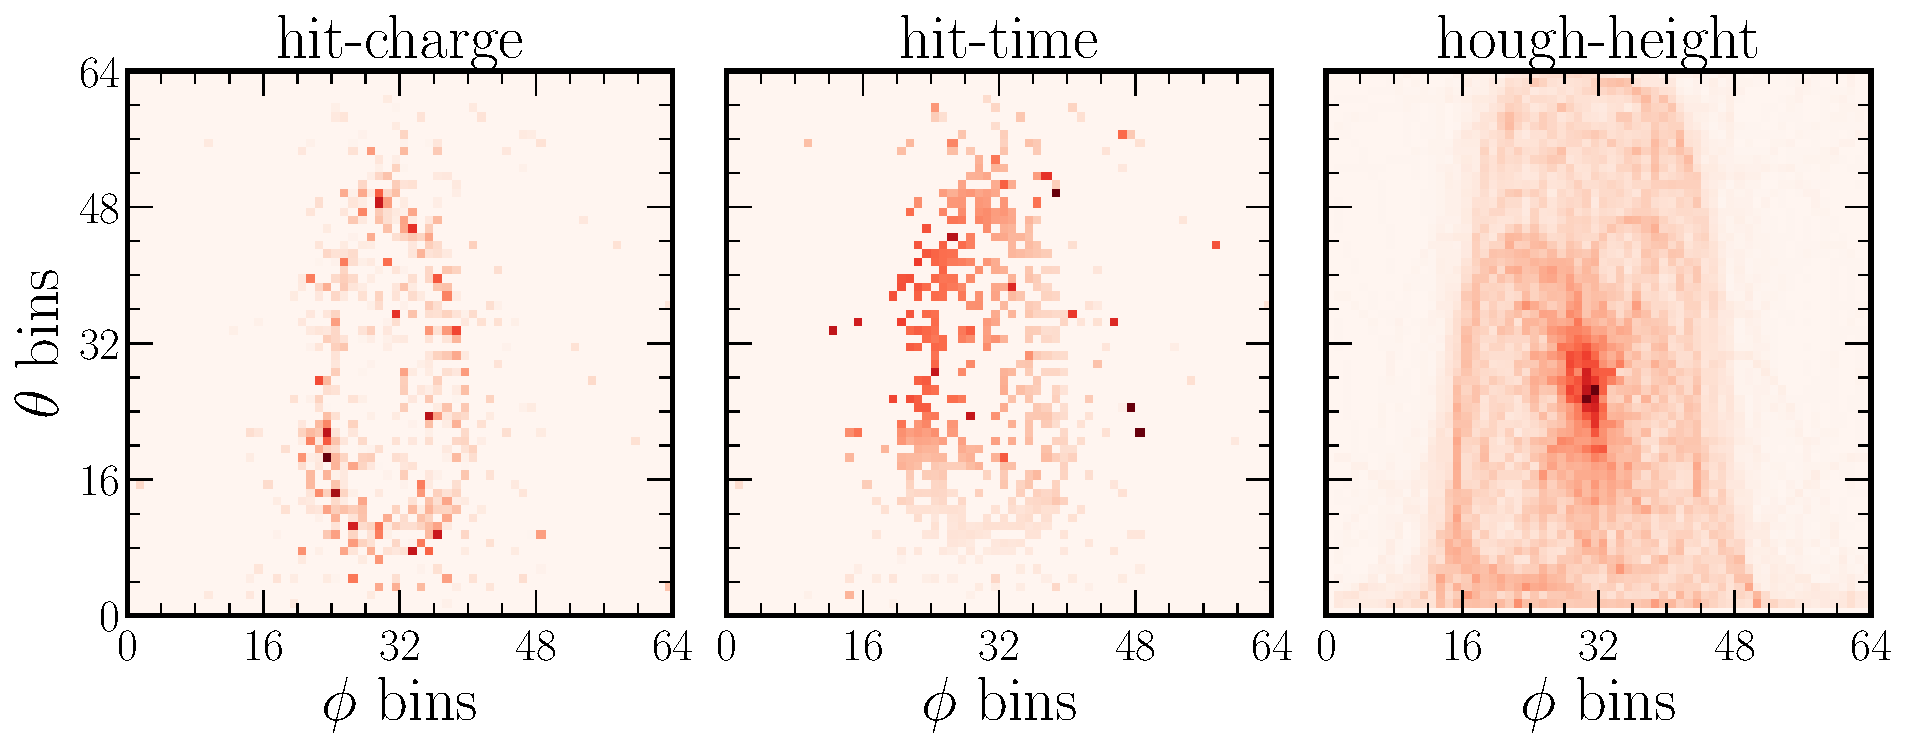
\includegraphics[width=\textwidth]{diagrams/7-results/explain_example_event.pdf}
    \caption[Example CC quasi-elastic $\nu_{e}$ event for explainability]
    {Three map representation of a CC quasi-elastic $\nu_{e}$ event. Initiated by a $\nu_{e}$ of
        energy \unit{2.4}{\GeV} with a final state $e^{-}$ of energy \unit{1.6}{\GeV}.}
    \label{fig:explain_example_event}
\end{figure}

\begin{figure} % ACTIVATIONS DIAGRAM %
    \centering
    \subcaptionbox{Cosmic rejection\label{fig:explain_cosmic_activations}}{%
        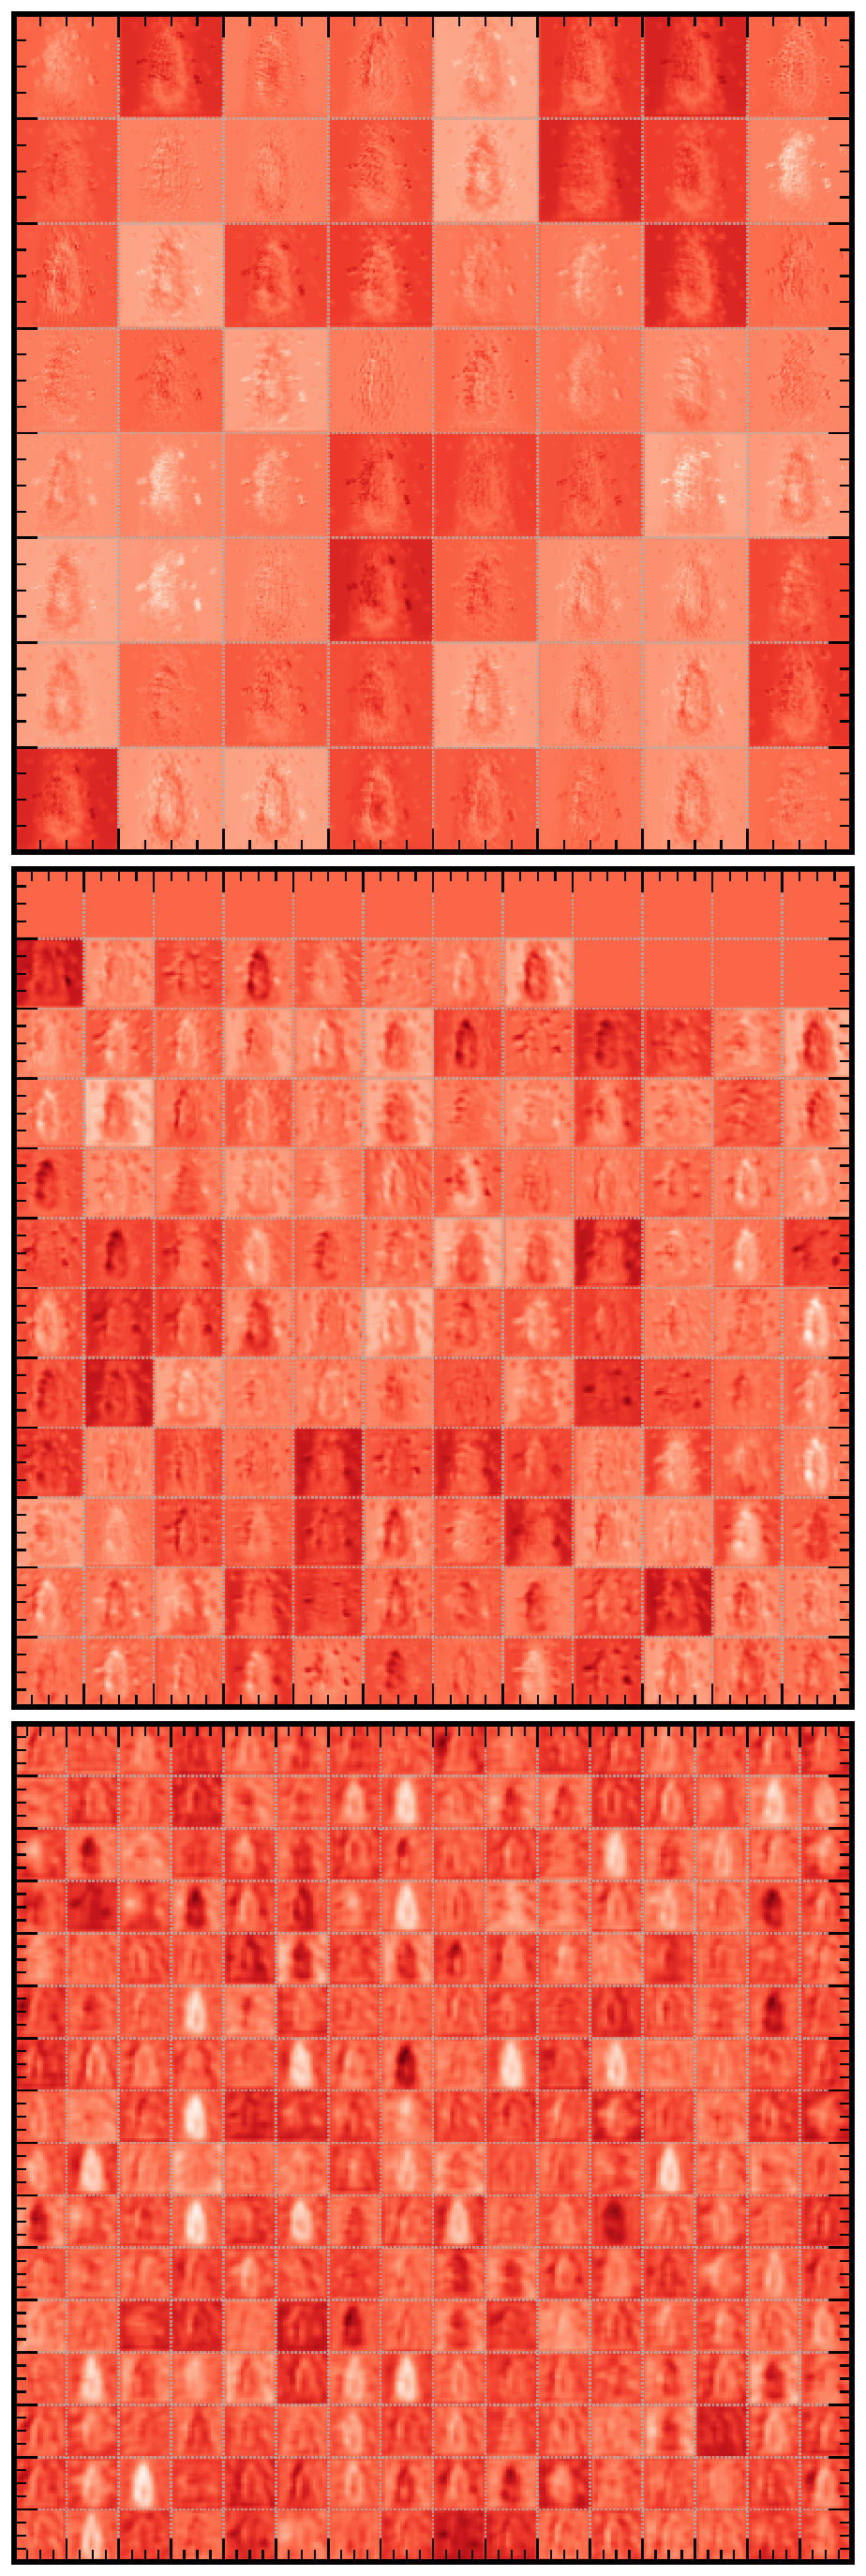
\includegraphics[height=14cm]{diagrams/7-results/explain_cosmic_activations.pdf}%
    }
    \quad
    \subcaptionbox{Beam classification\label{fig:explain_beam_activations}}{%
        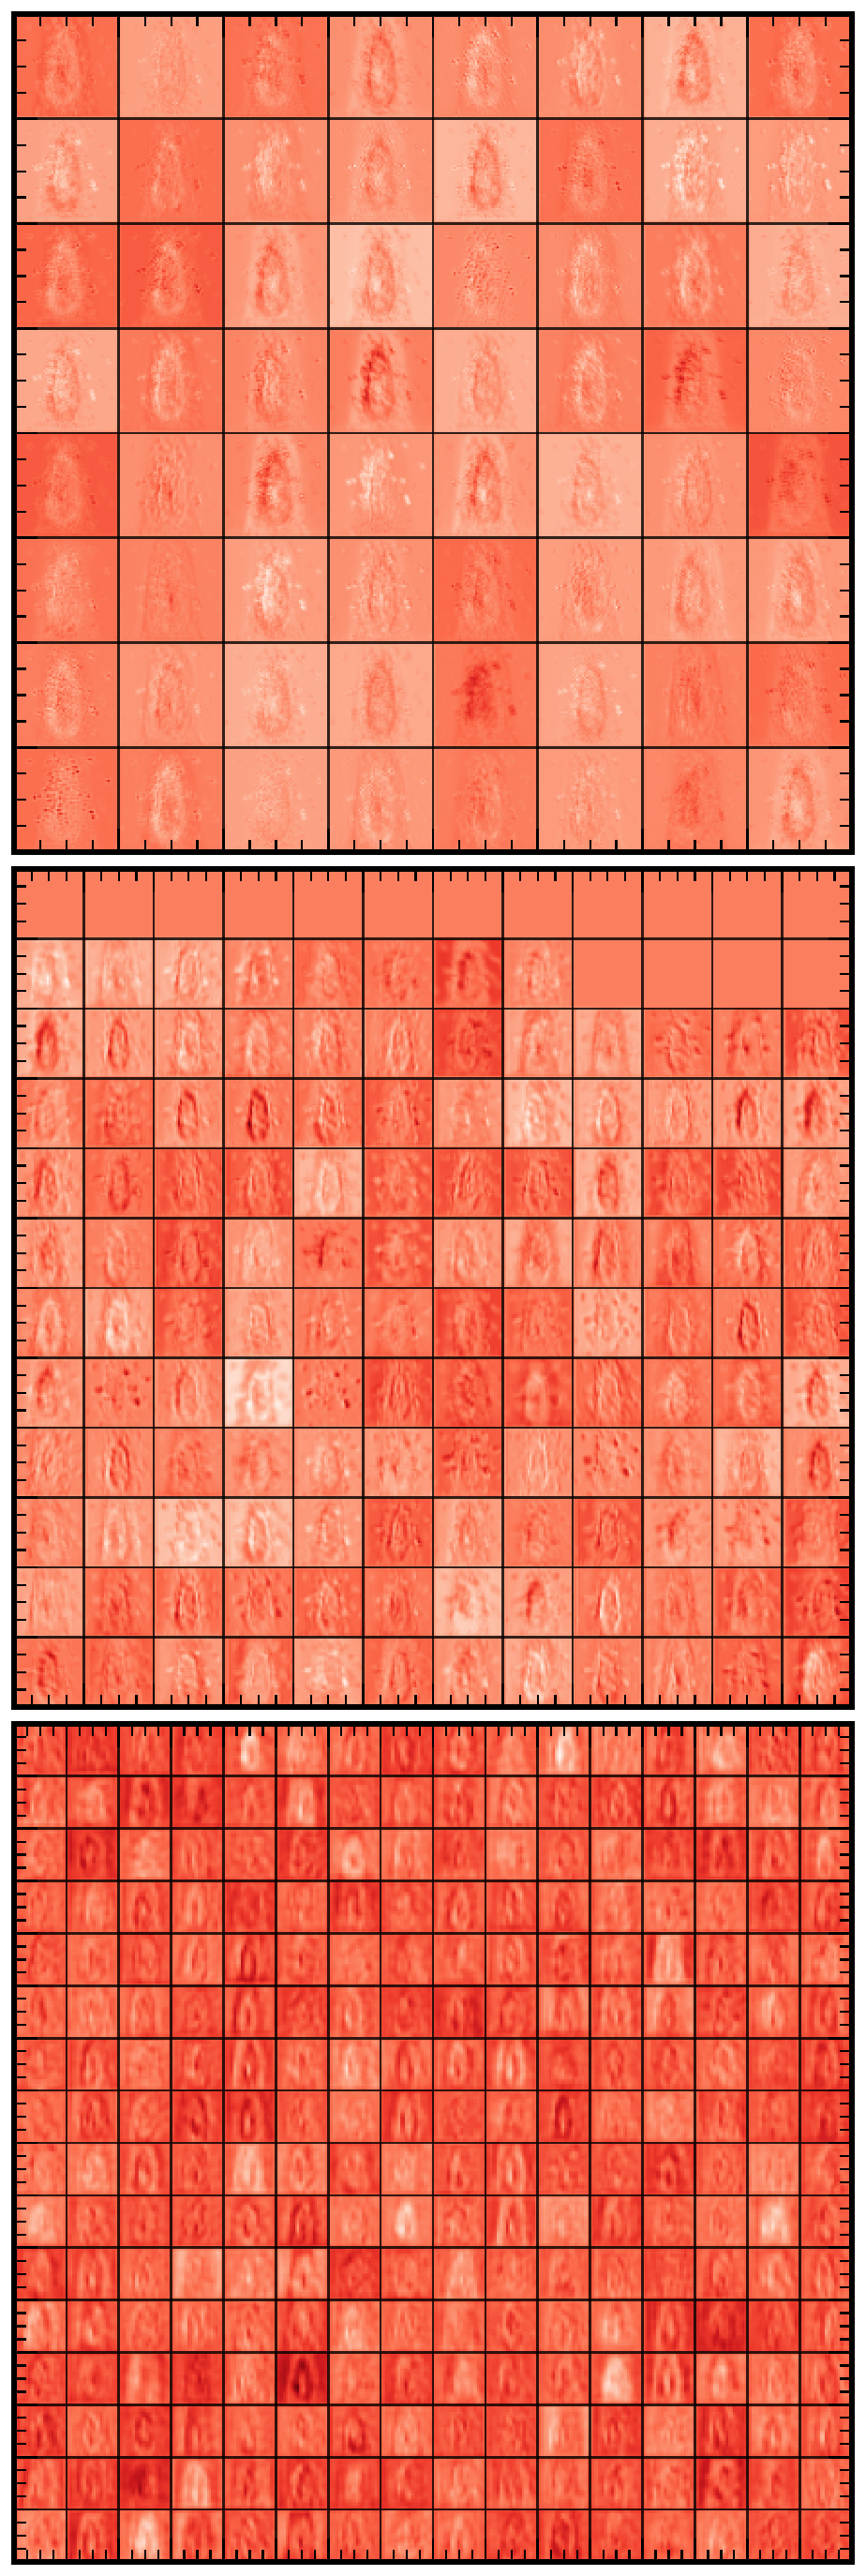
\includegraphics[height=14cm]{diagrams/7-results/explain_beam_activations.pdf}%
    }
    \quad
    \subcaptionbox{Energy estimation\label{fig:explain_energy_activations}}{%
        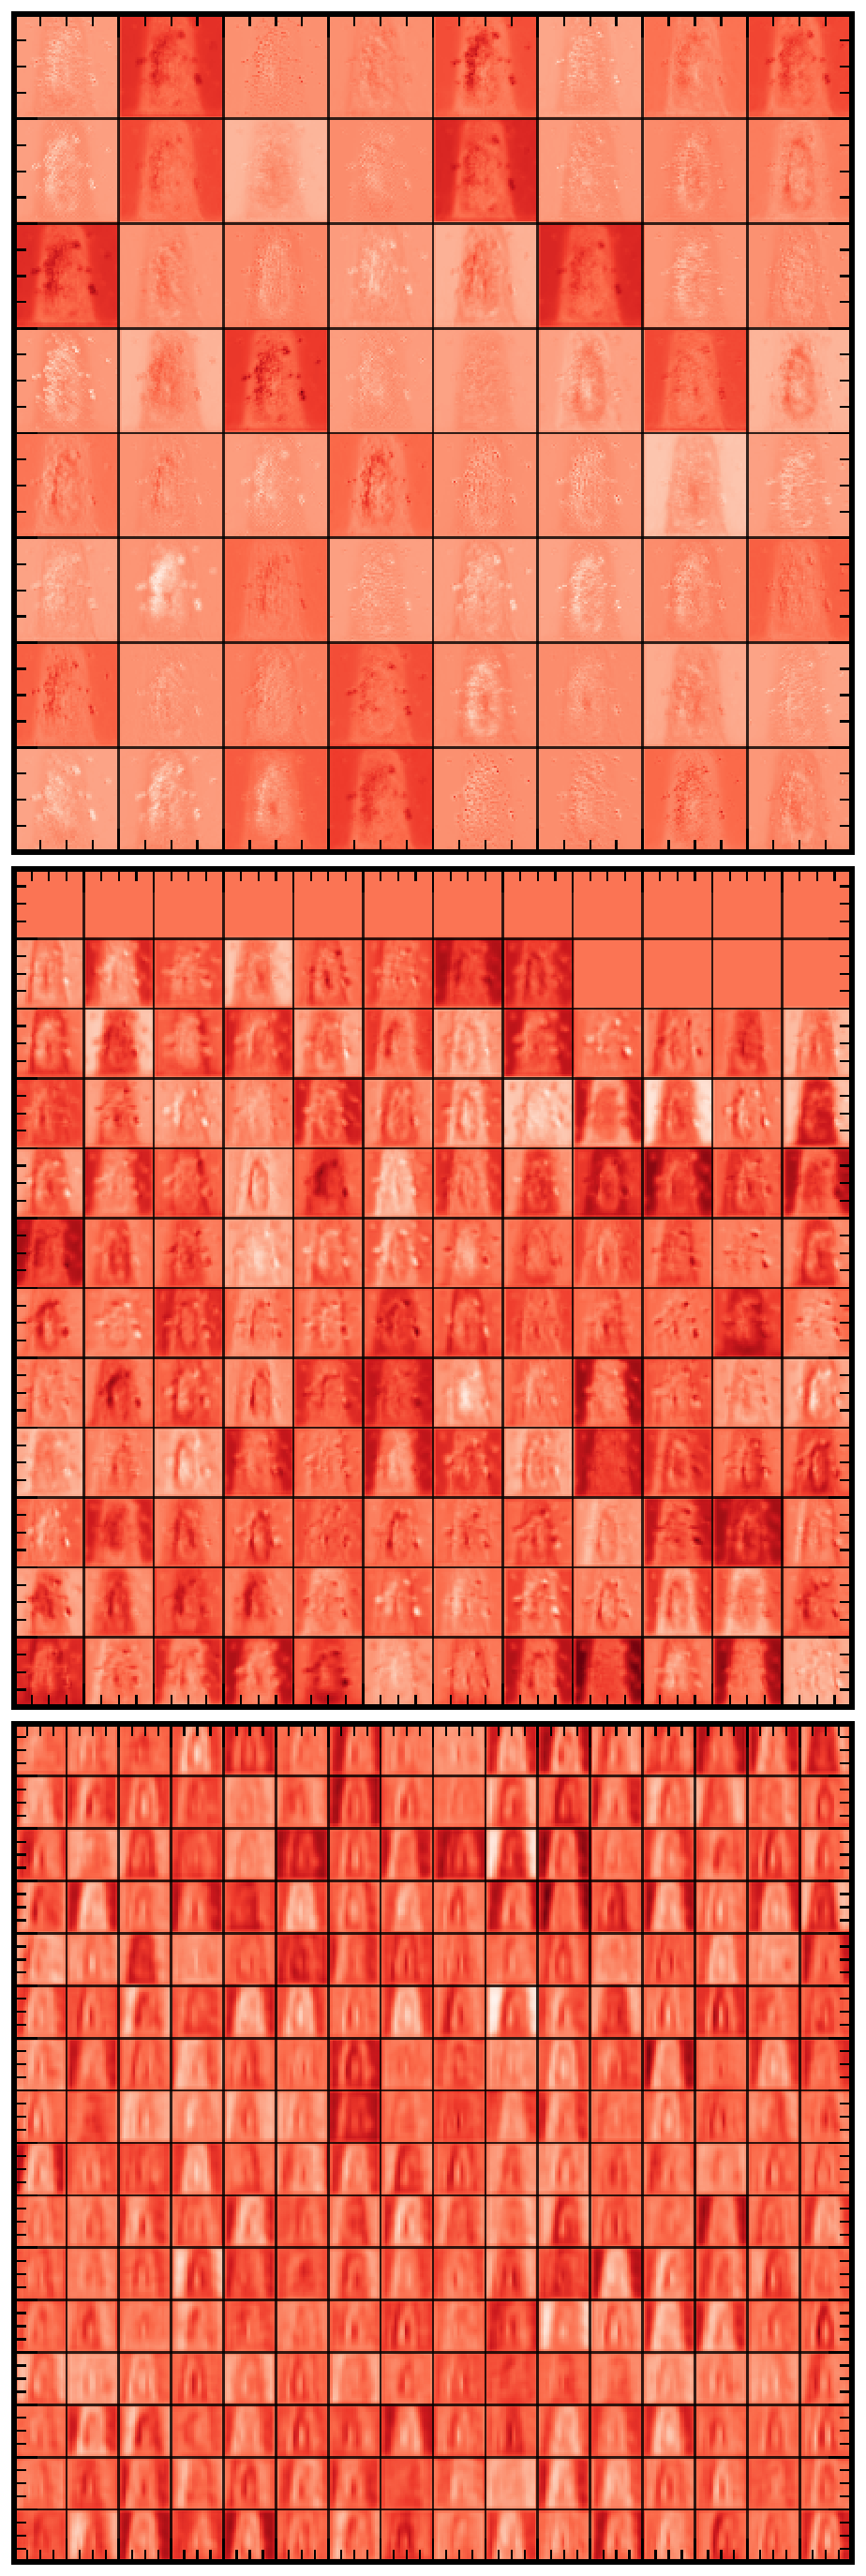
\includegraphics[height=14cm]{diagrams/7-results/explain_energy_activations.pdf}%
    }
    \caption[Visualisations of trained feature map outputs]
    {Visualisations of the feature map outputs using as input the event shown in
        Fig.~\ref{fig:explain_example_event}. Shown are the activated outputs from the first
        (top), the second (middle), and the third (bottom) VGG blocks for each of the trained
        network types. A chipsnet architecture with only a single branch and all three input event
        maps stacked into a single three-channel input image is used for simplicity.}
    \label{fig:cnn_visualisations}
\end{figure}

Another technique to analyse trained CNNs is t-Distributed Stochastic Neighbour embedding
(t-SNE)~\cite{maaten2008}. The t-SNE procedure is an unsupervised learning algorithm to visualise
the learnt high-dimensional feature-space of a trained network in two dimensions. It accomplishes
this by clustering events with similar features nearby in two-dimensional space and separating
events with dissimilar features. Here, the last fully connected layer before the network outputs
(512 dimensions) are used as input as they provide the best representation of the learnt network
features.

Visualisations of the t-SNE algorithm applied to both the trained cosmic rejection and beam
classification networks are shown in Fig.~\ref{fig:final_cosmic_tsne} and
Fig.~\ref{fig:final_beam_tsne} respectively. The very strong cosmic like to beam like separation
presented in the previous chapter is clear from the cosmic rejection visualisation. For the beam
classification network, as expected, the separation is weaker, with major overlap between
categories, especially CC $\nu_{e}$ and NC events.

For the beam classification network, three events, highlighted in t-SNE space, are shown in
Fig.~\ref{fig:final_beam_tsne_events}. Each event is highly representative of the corresponding
category achieving a high respective `combined category' score. Both the CC $\nu_{e}$ and NC
events shown are typical of that expected. However, the CC $\nu_{\mu}$ event clearly contains a
primary charged that escapes the detector (identified by the central peak). This suggests that
strongly classified CC $\nu_{\mu}$ are identified by this `escaping' feature rather than the shape
of the muon ring. Future work, therefore, should explore using only fully contained events during
beam classification training.

\begin{figure} % COSMIC t-SNE DIAGRAM %
    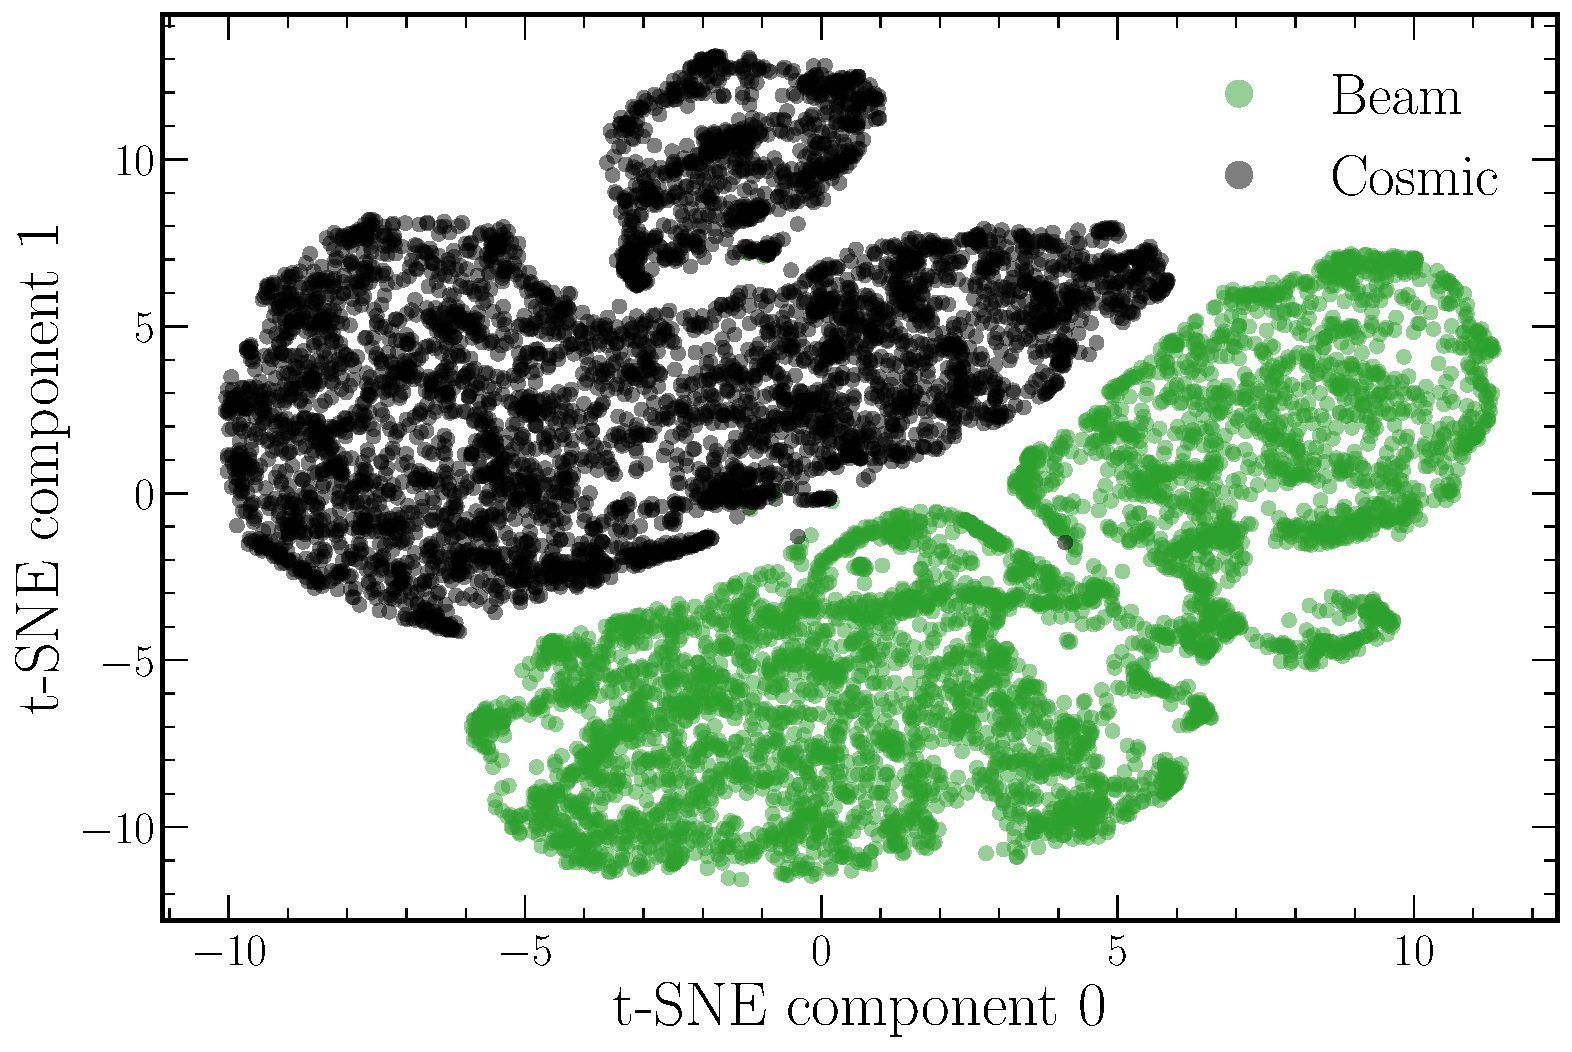
\includegraphics[width=\textwidth]{diagrams/7-results/final_cosmic_tsne.pdf}
    \caption[Cosmic rejection network t-SNE space]
    {Two dimensional probability space of beam and cosmic events generated using the t-SNE
        procedure on the final fully-connected layer of the trained cosmic rejection network.}
    \label{fig:final_cosmic_tsne}
\end{figure}

\begin{figure} % BEAM t-SNE DIAGRAM %
    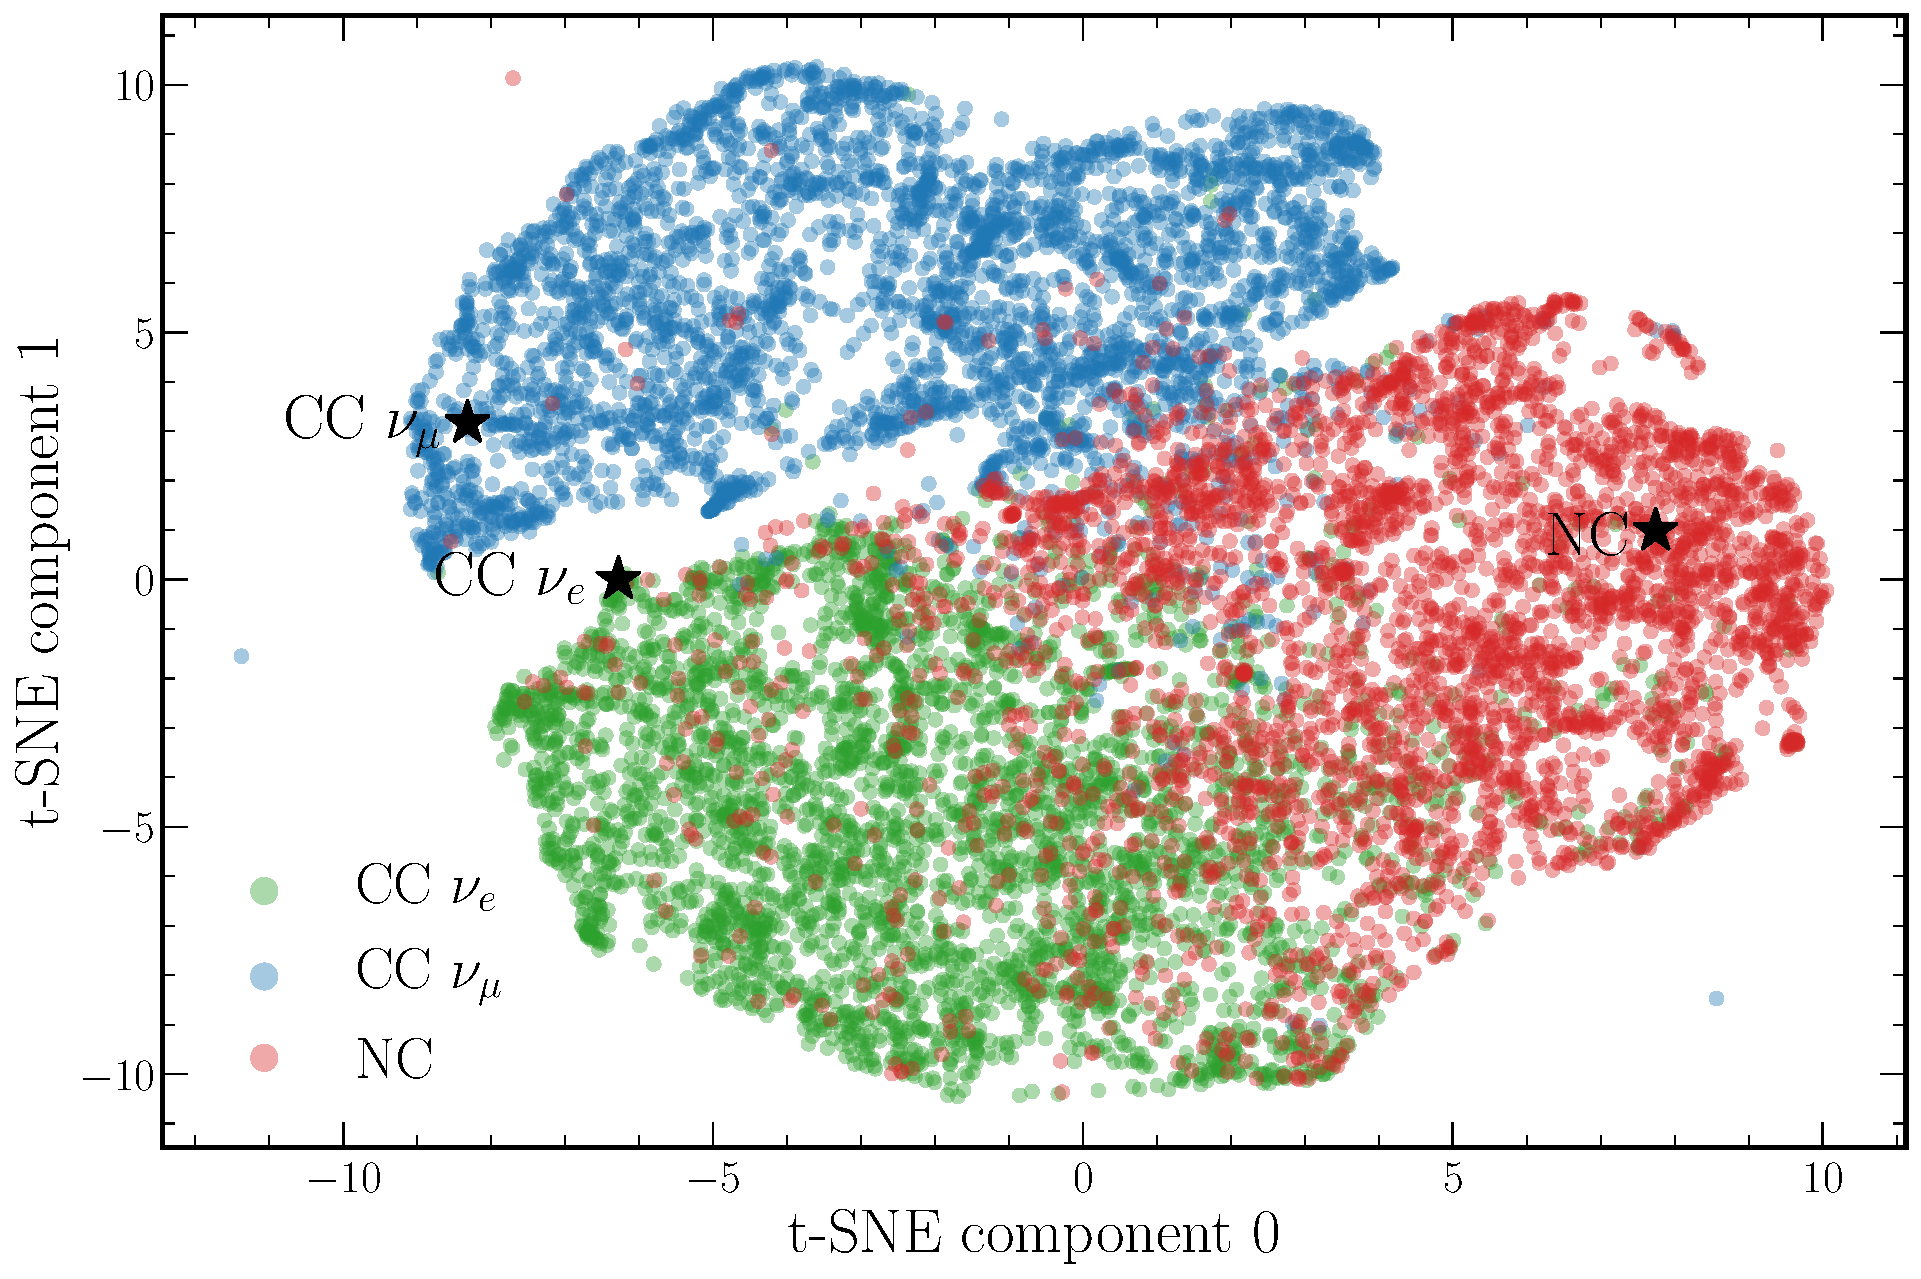
\includegraphics[width=\textwidth]{diagrams/7-results/final_beam_tsne.pdf}
    \caption[Beam classification network t-SNE space]
    {Two dimensional probability space of different beam events generated using the t-SNE
        procedure on the final fully-connected layer of the trained beam classification network.
        Three events, one highly CC $\nu_{e}$ like, one highly CC $\nu_{\mu}$ like, and one highly
        NC like are highlighted and shown in Fig.~\ref{fig:final_beam_tsne_events}.}
    \label{fig:final_beam_tsne}
\end{figure}

\begin{figure} % BEAM t-SNE EVENTS DIAGRAM %
    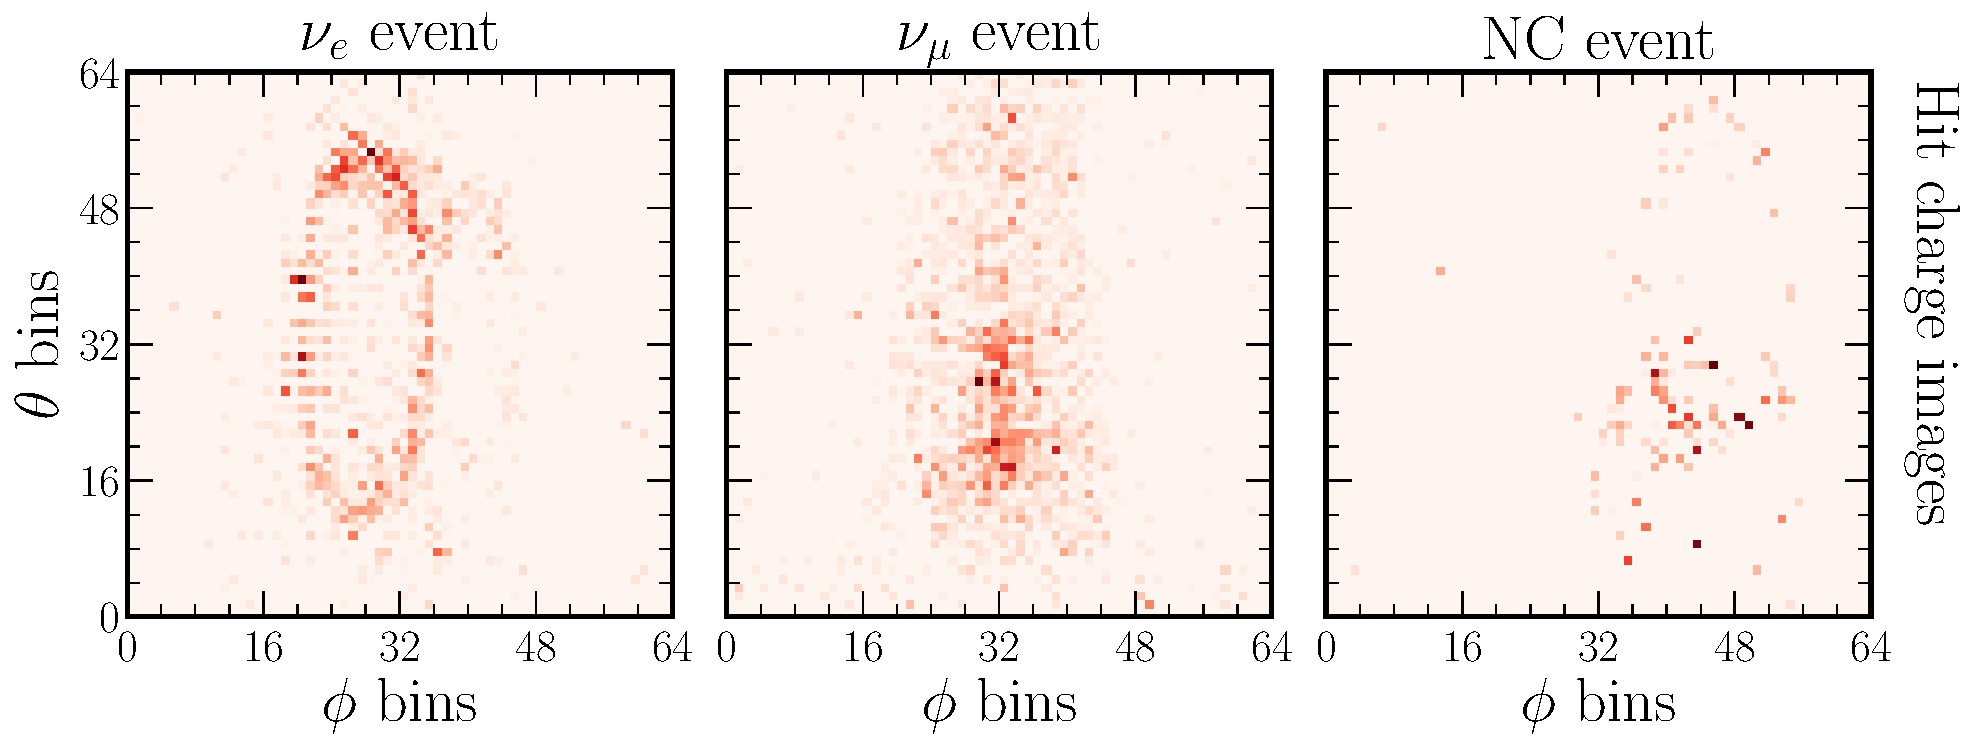
\includegraphics[width=\textwidth]{diagrams/7-results/final_beam_tsne_events.pdf}
    \caption[Hit-charge maps of highly CC $\nu_{e}$ like, CC $\nu_{\mu}$ like, and NC like events]
    {Hit-charge maps of the most CC $\nu_{e}$ like, CC $\nu_{\mu}$ like, and NC like events from
        Fig.~\ref{fig:final_beam_tsne}.}
    \label{fig:final_beam_tsne_events}
\end{figure}

\section{Robustness} %%%%%%%%%%%%%%%%%%%%%%%%%%%%%%%%%%%%%%%%%%%%%%%%%%%%%%%%%%%%%%%%%%%%%%%%%%%%%
\label{sec:results_robust} %%%%%%%%%%%%%%%%%%%%%%%%%%%%%%%%%%%%%%%%%%%%%%%%%%%%%%%%%%%%%%%%%%%%%%%

- Go back and mention how augmentation in the implementation hopes to make the models more robust.
What are the things we need to be robust against? Mainly the calibration, wrong Monte Carlo etc,
position, time, charge are the things that can chance about the input, position is obviously
robust as our bins are 2.5m is theta and 2m in phi approx (when viewed from the centre of the
detector), this means the absolute position of PMTs is not very important in the context of the
networks trained here, maybe future work could look at making the images bigger, but did that hee
to speed up optimisation process and make training not take too long.

\subsection*{Time calibration} %%%%%%%%%%%%%%%%%%%%%%%%%%%%%%%%%%%%%%%%%%%%%%%%%%%%%%%%%%%%%%%%%%%

\begin{figure} % CALIB TIME NUEL EFF CURVES DIAGRAM %
    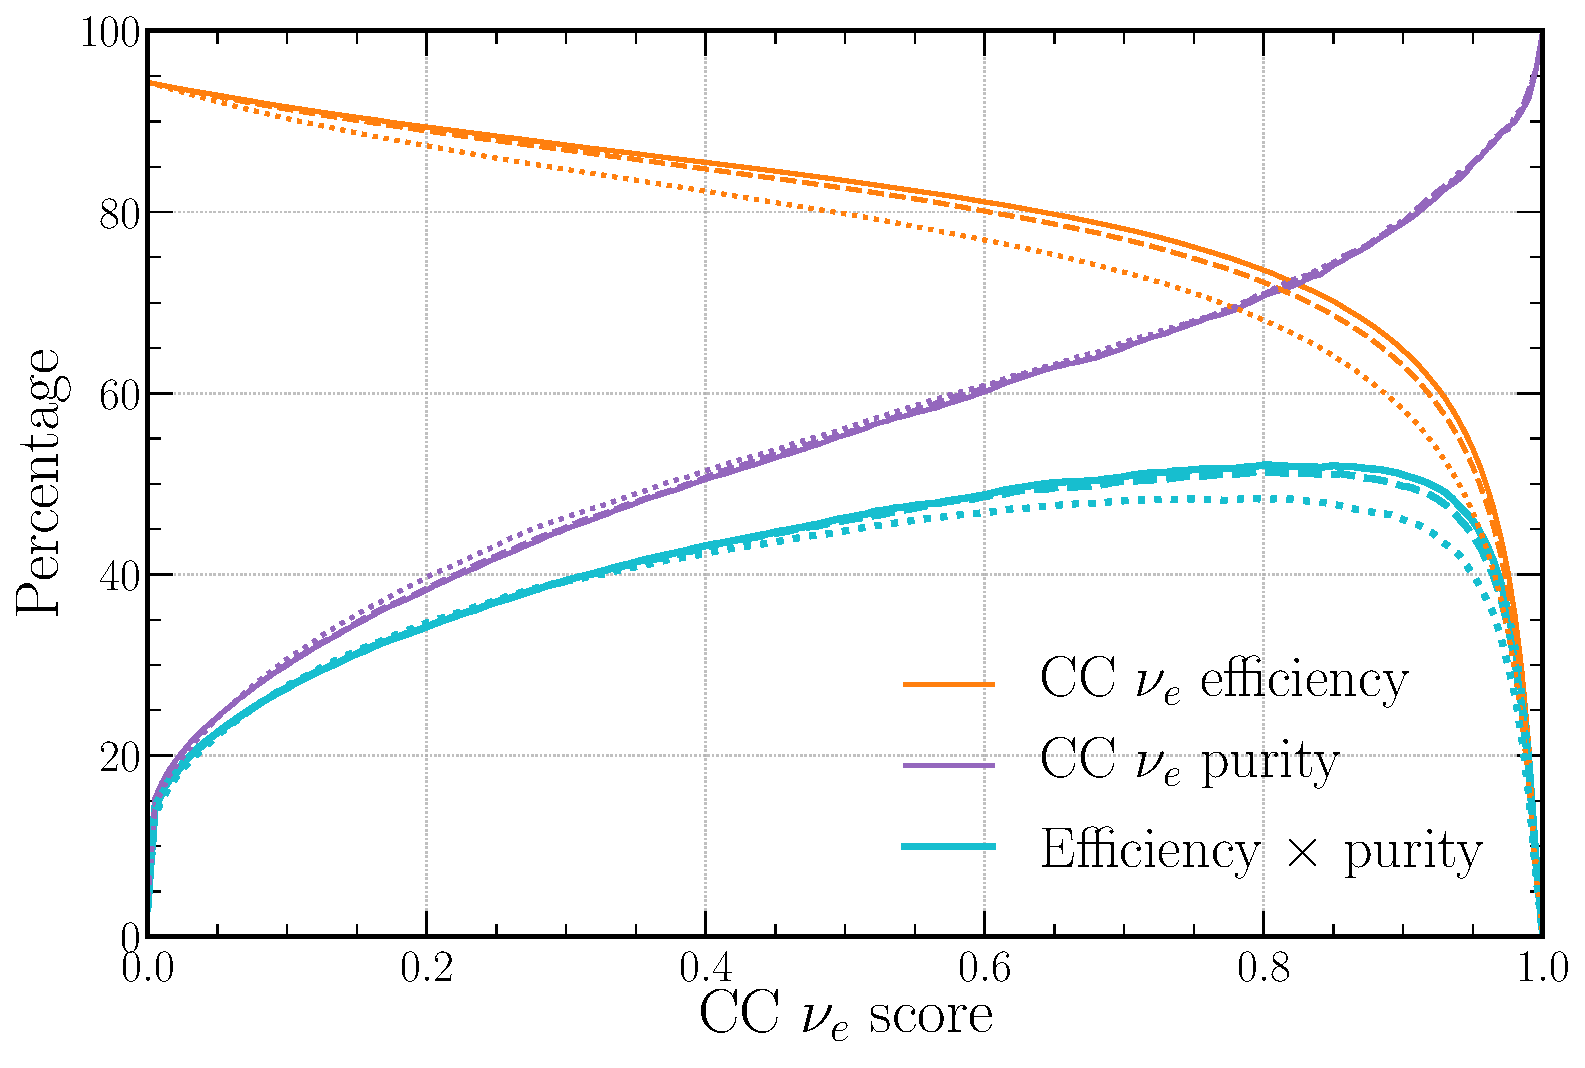
\includegraphics[width=0.7\textwidth]{diagrams/7-results/calib_time_nuel_eff_curves.pdf}
    \caption[CC $\nu_{e}$ efficiency and purity curves for the three input image representations]
    {CC $\nu_{e}$ efficiency, purity and $\mathrm{efficiency}\times\mathrm{purity}$ for different
        values of CC $\nu_{e}$ score selection for the three input image representations
        considered. The \emph{vertex view} curves are shown by the solid lines, the \emph{origin
            raw view} curves by the dashed lines, and the \emph{origin dotted} surves by the dotted
        lines.}
    \label{fig:calib_time_nuel_eff_curves}
\end{figure}

\begin{figure} % CALIB TIME NUEL COMP CURVES DIAGRAM %
    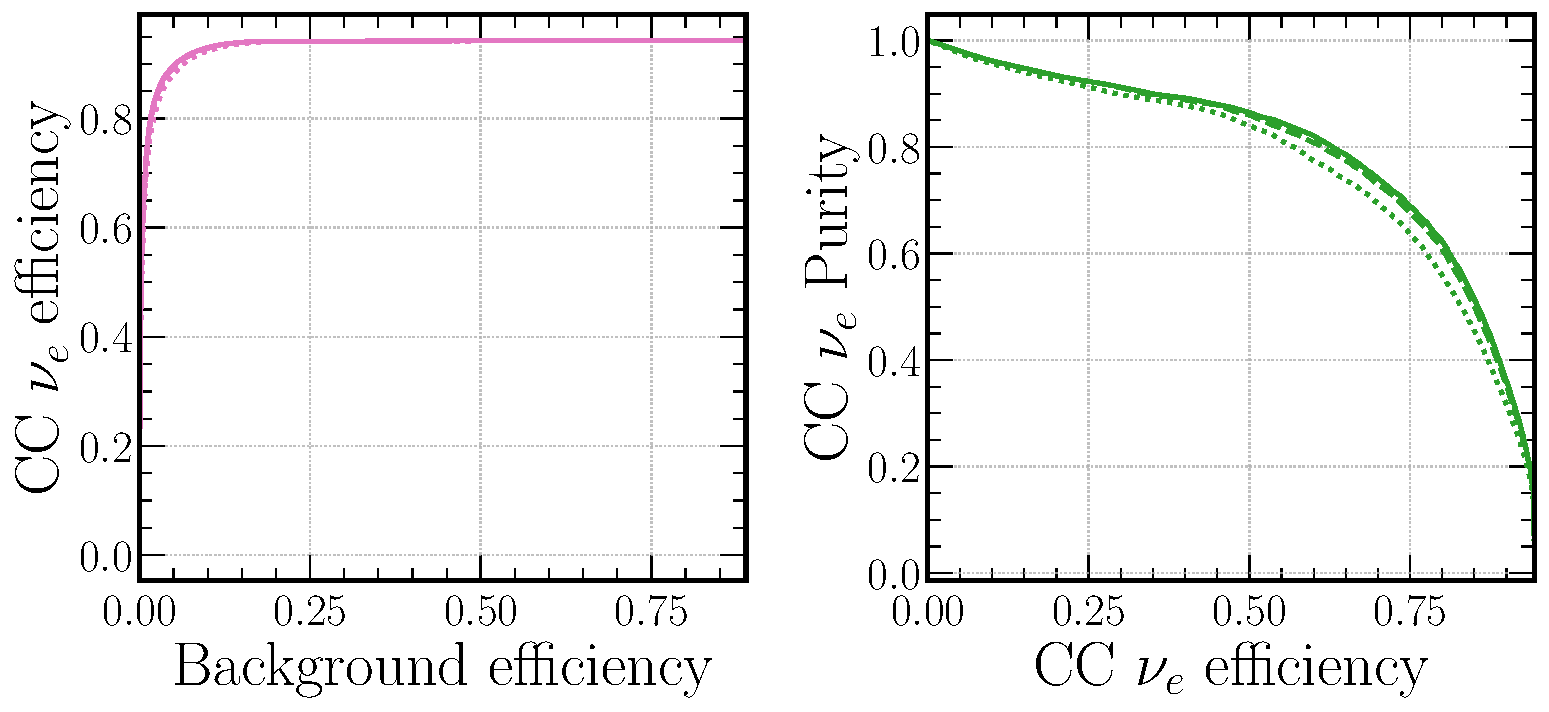
\includegraphics[width=0.7\textwidth]{diagrams/7-results/calib_time_nuel_comp_curves.pdf}
    \caption[CC $\nu_{e}$ efficiency and purity curves for the three input image representations]
    {CC $\nu_{e}$ efficiency, purity and $\mathrm{efficiency}\times\mathrm{purity}$ for different
        values of CC $\nu_{e}$ score selection for the three input image representations
        considered. The \emph{vertex view} curves are shown by the solid lines, the \emph{origin
            raw view} curves by the dashed lines, and the \emph{origin dotted} surves by the dotted
        lines.}
    \label{fig:calib_time_nuel_comp_curves}
\end{figure}

\subsection*{Charge calibration} %%%%%%%%%%%%%%%%%%%%%%%%%%%%%%%%%%%%%%%%%%%%%%%%%%%%%%%%%%%%%%%%%

\subsection*{Random noise} %%%%%%%%%%%%%%%%%%%%%%%%%%%%%%%%%%%%%%%%%%%%%%%%%%%%%%%%%%%%%%%%%%%%%%%

\section{Alternative implementations} %%%%%%%%%%%%%%%%%%%%%%%%%%%%%%%%%%%%%%%%%%%%%%%%%%%%%%%%%%%%
\label{sec:results_alt} %%%%%%%%%%%%%%%%%%%%%%%%%%%%%%%%%%%%%%%%%%%%%%%%%%%%%%%%%%%%%%%%%%%%%%%%%%

Here we present a sample of alternative (but not as good) implementation as they help understand
which factors are important for network performance, just look at beam classification as this is
the main one, these findings translate to both the cosmic rejection and energy estimation networks
also, extensive testing, this is just a selection of the findings from that process also hints and
informs our choice of future work.

\subsection*{Alternative inputs} %%%%%%%%%%%%%%%%%%%%%%%%%%%%%%%%%%%%%%%%%%%%%%%%%%%%%%%%%%%%%%%%%
% The way you represent the event as an image has a significant impact on performance
% The different channels don't provide a huge improvement over a single one

- Many different possible event representation, three different ones considered in this work, a
simple theta and phi view from the origin and a new idea for constant PMT density with x+ x-
mapping in Ref.~\cite{berns2020}, fraction of deposited charge in endcaps is 48\%

\begin{equation} % ISO CASE EQUATION %
    X_{\pm}=
    \begin{cases}
        1-\chi_{\mp} & (z \geq 0) \\
        \chi_{\pm}   & (z < 0)
    \end{cases}
    \label{eq:iso_case}
\end{equation}

\begin{equation} % ISO MAIN EQUATION %
    \chi_{\pm}=W(\rho,z)\frac{\pi\pm\phi}{2\pi}
    \label{eq:iso_main}
\end{equation}

\begin{equation} % ISO PART EQUATION %
    W(\rho,z)=\sqrt{\frac{\rho^{2}-2R|z|+RH}{R^{2}+RH}}
    \label{eq:iso_part}
\end{equation}

- where R and Z are the radius and height of the detector cylinder and W is chosen for constant
surface density.
- Turns out removing the distortions of not viewing the event from the vertex is the most
important thing!!!

- Approaches in the past for event classification using CNNs for water cherenkov detectors have
taken a few Approaches to generating the input image representation.
- Projecting onto a 2d surface "outside" the detector

\begin{table}
    \begin{tabular}{cccc}
        Metric                   & Vertex View & Origin Raw View & Origin Iso View \\
        \midrule
        Maximum FOM              & 0.461       & 0.422           & 0.419           \\
        Highest Score Efficiency & 0.878       & 0.874           & 0.867           \\
        Highest Score Purity     & 0.354       & 0.291           & 0.298           \\
        ROC Integral             & 0.825       & 0.822           & 0.821           \\
        PRC Integral             & 0.707       & 0.675           & 0.670           \\
    \end{tabular}
    \caption[Comparison of performance metrics for three input image representations.]
    {Comparison of performance metrics for the three input image representations considered. The
        highest score selection uses the highest scoring output neuron for classification. The ROC
        and PRC integrals are taken from the curves shown in
        Fig.~\ref{fig:repr_nuel_comp_curves}.}
    \label{tab:repr}
\end{table}

\begin{figure} % REPR NUEL EFF CURVES DIAGRAM %
    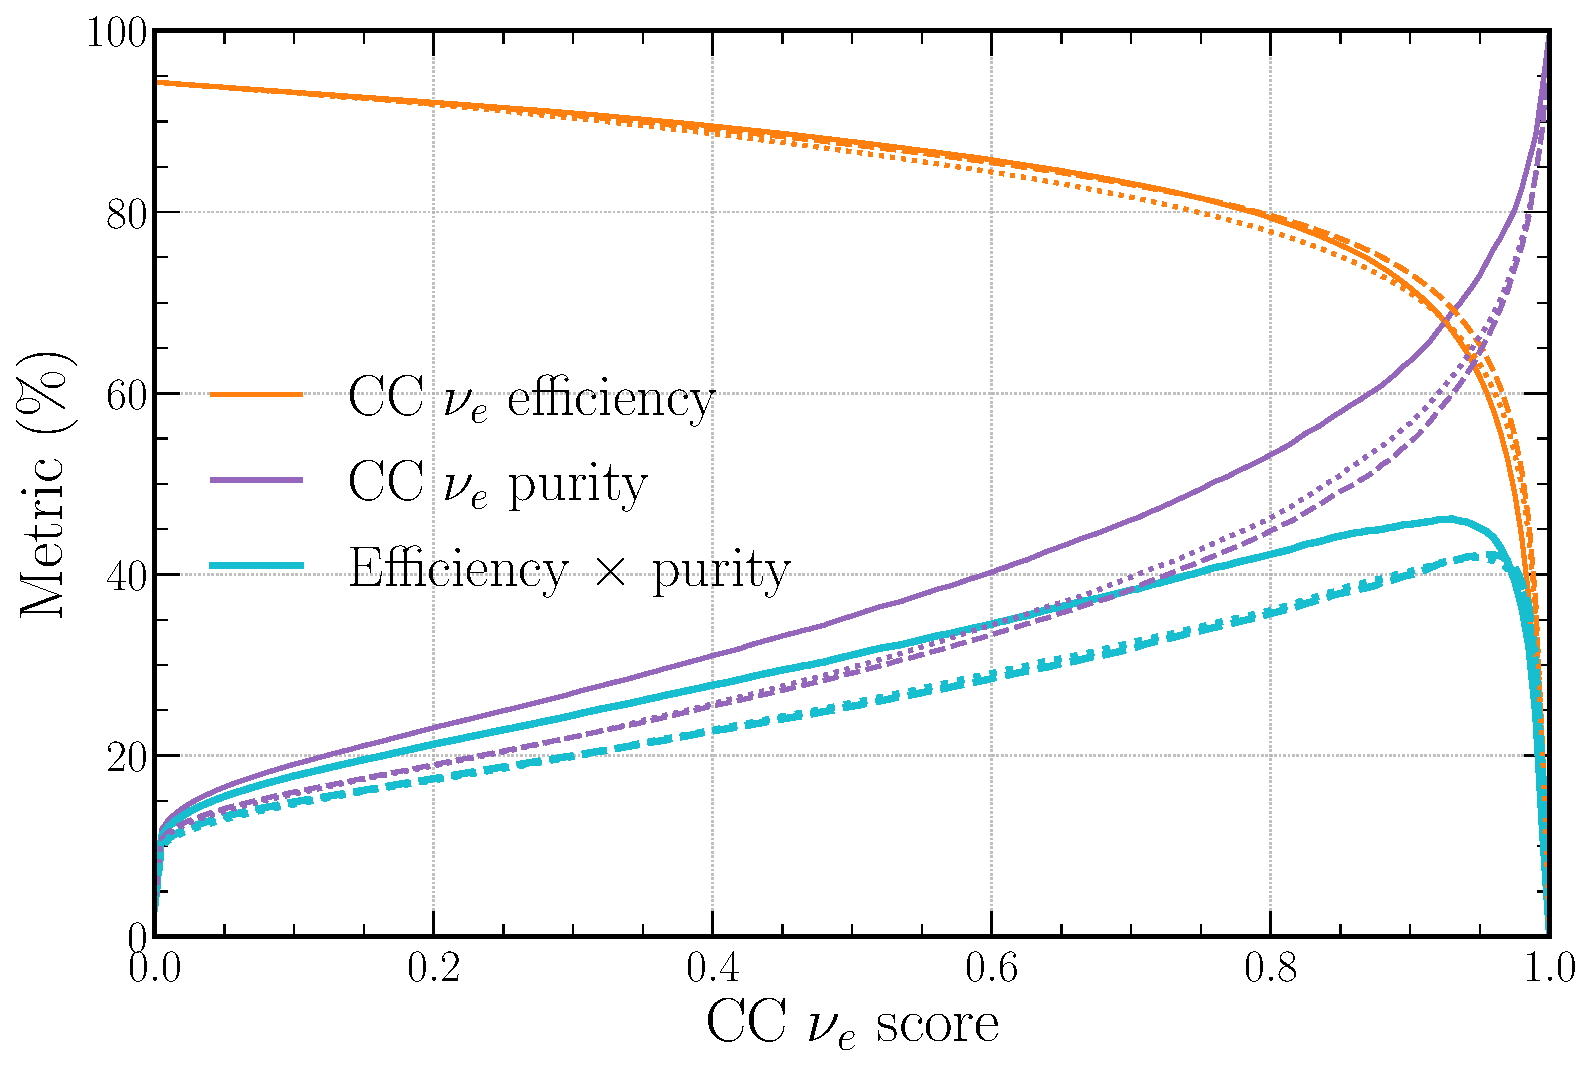
\includegraphics[width=0.7\textwidth]{diagrams/7-results/repr_nuel_eff_curves.pdf}
    \caption[CC $\nu_{e}$ efficiency and purity curves for the three input image representations]
    {CC $\nu_{e}$ efficiency, purity and $\mathrm{efficiency}\times\mathrm{purity}$ for different
        values of CC $\nu_{e}$ score selection for the three input image representations
        considered. The \emph{vertex view} curves are shown by the solid lines, the \emph{origin
            raw view} curves by the dashed lines, and the \emph{origin dotted} surves by the dotted
        lines.}
    \label{fig:repr_nuel_eff_curves}
\end{figure}

\begin{figure} % REPR NUEL COMP CURVES DIAGRAM %
    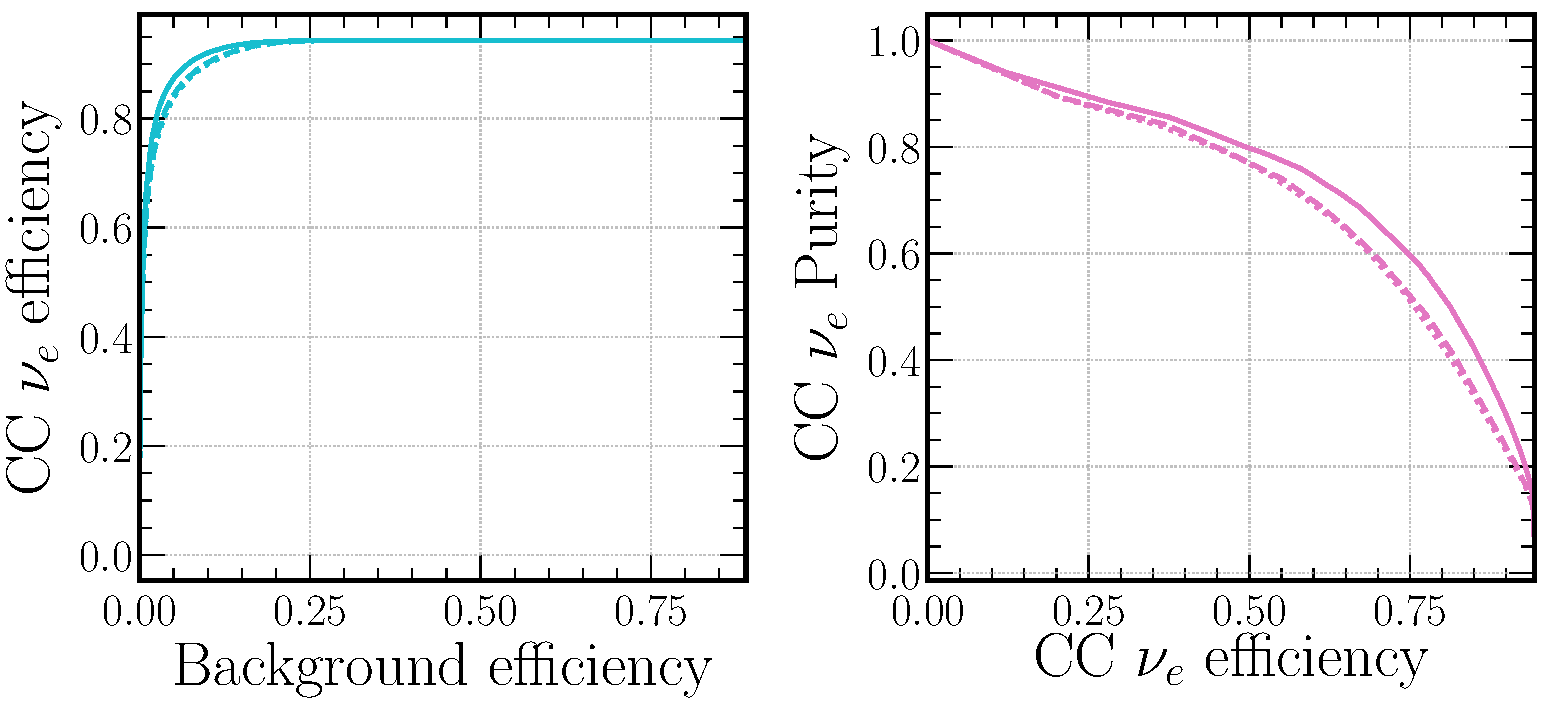
\includegraphics[width=0.8\textwidth]{diagrams/7-results/repr_nuel_comp_curves.pdf}
    \caption[Comparison curves for the three input image representations considered]
    {Comparison curves for the three input image representations considered. Signal vs background
        selection efficiencies as the CC $\nu_{e}$ score selection is varied (left). Signal CC
        $\nu_{e}$ purity vs efficiency as the CC $\nu_{e}$ score selection is varied (right). The
        \emph{vertex view} curves are shown by the solid lines, the \emph{origin raw view} curves
        by the dashed lines, and the \emph{origin dotted} curves by the dotted lines. The left
        plot contains what are commonly referred to as receiver-operator curves (ROC), while the
        right plot contains precision-recall (PRC) curves.}
    \label{fig:repr_nuel_comp_curves}
\end{figure}

\begin{table}
    \begin{tabular}{cccc}
        Metric                   & Charge & Charge+Time & Charge+Time+Hough \\
        \midrule
        Maximum FOM              & 0.436  & 0.461       & 0.465             \\
        Highest Score Efficiency & 0.869  & 0.878       & 0.877             \\
        Highest Score Purity     & 0.357  & 0.354       & 0.369             \\
        ROC Integral             & 0.824  & 0.825       & 0.826             \\
        PRC Integral             & 0.689  & 0.707       & 0.712             \\
    \end{tabular}
    \caption[Comparison of performance metrics for each additional input image map.]
    {Comparison of performance metrics for each additional input image map. The highest score
        selection uses the highest scoring output neuron for classification.}
    \label{tab:chan}
\end{table}

\subsection*{Alternative training samples} %%%%%%%%%%%%%%%%%%%%%%%%%%%%%%%%%%%%%%%%%%%%%%%%%%%%%%%
% Using a training sample representative of the expected event composition is very important.

- It may be tempting to use the same number of training samples from each category, but this is
not found to improve performance, shows that the network does use an averaging technique to some
degree. This is not the same for energy estimation, that may be better to use a uniform one in
energy.

\begin{figure} % REPR NUEL EFF CURVES DIAGRAM %
    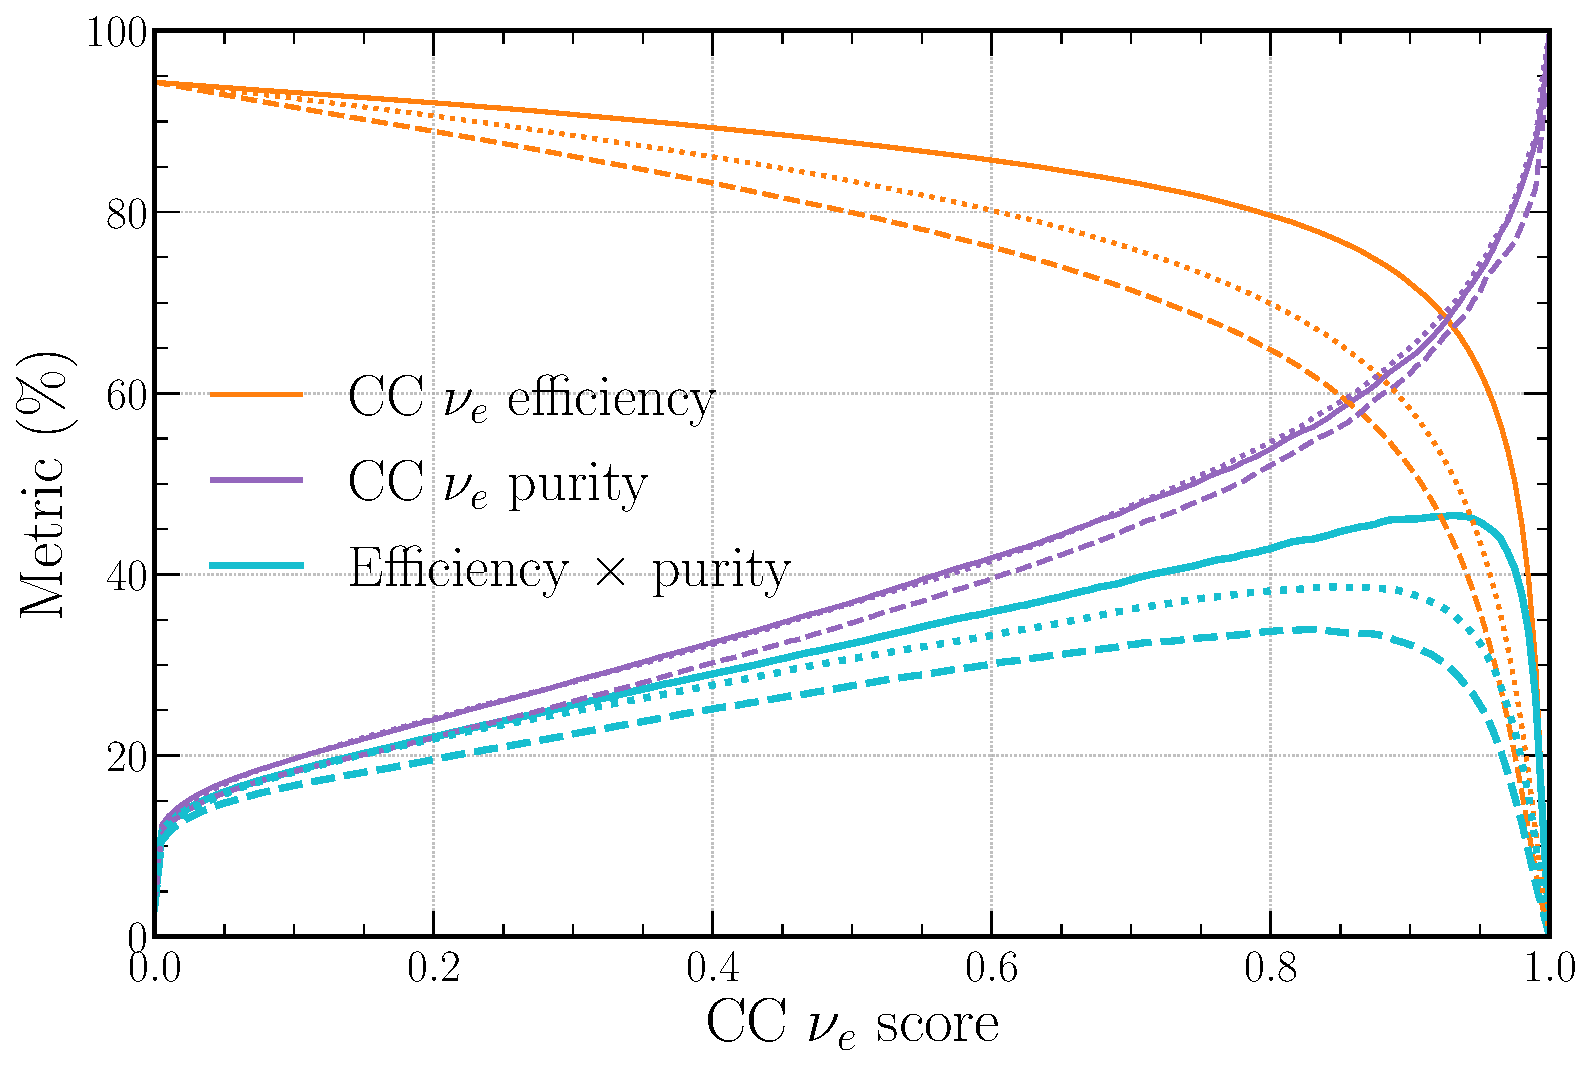
\includegraphics[width=0.7\textwidth]{diagrams/7-results/sample_nuel_eff_curves.pdf}
    \caption[CC $\nu_{e}$ efficiency and purity curves for the different training samples]
    {CC $\nu_{e}$ efficiency, purity and $\mathrm{efficiency}\times\mathrm{purity}$ for different
        values of CC $\nu_{e}$ score selection for the different training samples considered. The
        \emph{vertex view} curves are shown by the solid lines, the \emph{origin raw view} curves
        by the dashed lines, and the \emph{origin dotted} curves by the dotted lines.}
    \label{fig:sample_nuel_eff_curves}
\end{figure}

\begin{figure} % REPR NUEL COMP CURVES DIAGRAM %
    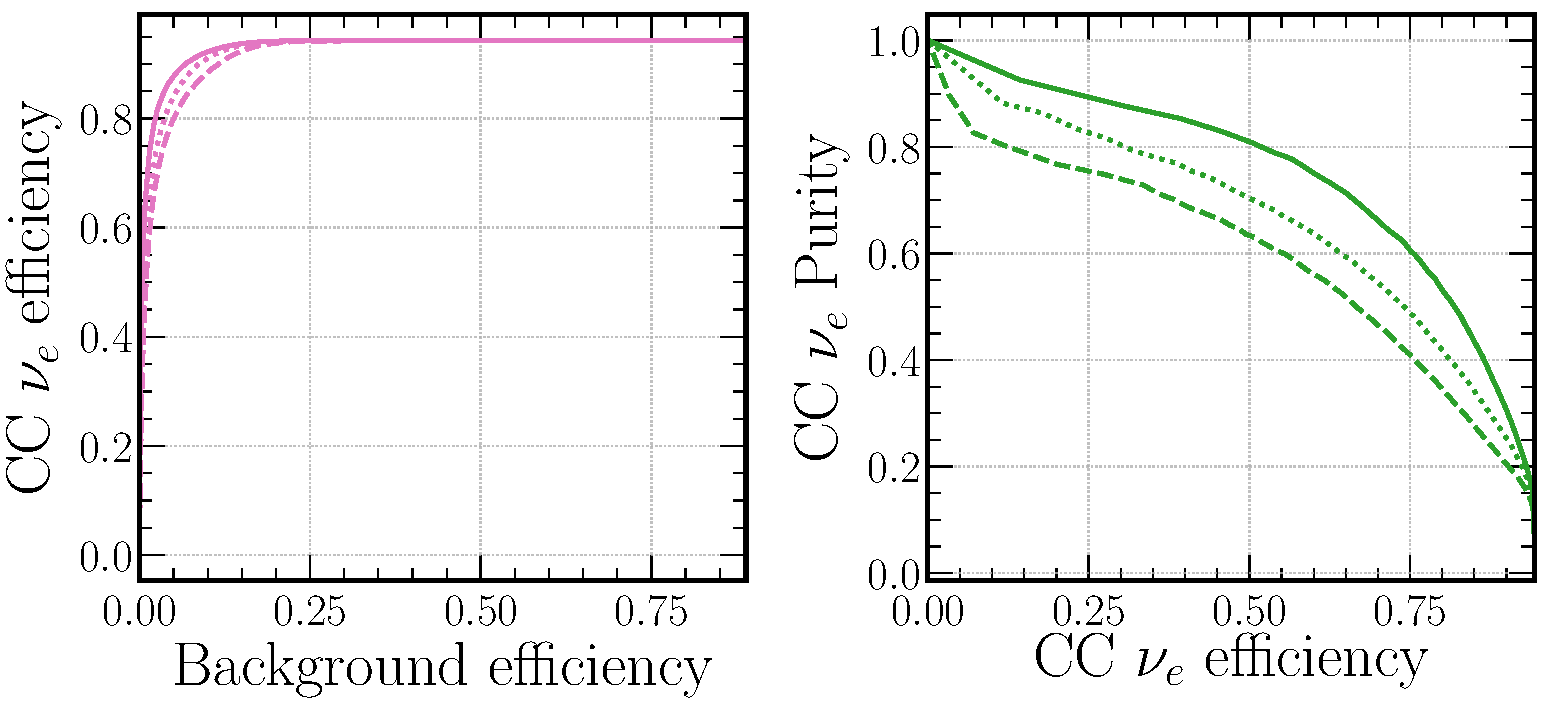
\includegraphics[width=0.8\textwidth]{diagrams/7-results/sample_nuel_comp_curves.pdf}
    \caption[Comparison curves for the different training samples considered]
    {Comparison curves for the different training samples considered. Signal vs background
        selection efficiencies as the CC $\nu_{e}$ score selection is varied (left). Signal CC
        $\nu_{e}$ purity vs efficiency as the CC $\nu_{e}$ score selection is varied (right). The
        \emph{flux+uniform} curves are shown by the solid lines, the \emph{flux} curves by the
        dashed lines, and the \emph{uniform} curves by the dotted lines. The left plot contains
        what are commonly referred to as receiver-operator curves (ROC), while the right plot
        contains precision-recall (PRC) curves.}
    \label{fig:sample_nuel_comp_curves}
\end{figure}

\begin{table}
    \begin{tabular}{cccc}
        Metric                   & Flux  & Uniform & Flux+Uniform \\
        \midrule
        Maximum FOM              & 0.465 & 0.339   & 0.386        \\
        Highest Score Efficiency & 0.877 & 0.799   & 0.834        \\
        Highest Score Purity     & 0.369 & 0.347   & 0.368        \\
        ROC Integral             & 0.826 & 0.815   & 0.820        \\
        PRC Integral             & 0.712 & 0.568   & 0.634        \\
    \end{tabular}
    \caption[Comparison of performance metrics for the different training samples considered.]
    {Comparison of performance metrics for the different training samples considered. The highest
        score selection uses the highest scoring output neuron for classification.}
    \label{tab:sample}
\end{table}

\subsection*{Alternative architectures} %%%%%%%%%%%%%%%%%%%%%%%%%%%%%%%%%%%%%%%%%%%%%%%%%%%%%%%%%%
% The network architecture doesn't seem to matter, easy problem, use fastest

- The network architecture is not found to matter that much, we tested on truncated versions of
other networks, all roughly same number of parameters for comparison, maybe that larger images
would allow these network to become better, possibility for future work to explore this.

\begin{table}
    \begin{tabular}{ccccc}
        Metric                   & VGG        & Inception  & ResNet     & Inception-ResNet \\
        \midrule
        Number of parameters     & 17,225,296 & 16,893,216 & 16,526,288 & 17,145,238       \\
        Iteration time (ms)      & 88         & 192        & 112        & 209              \\
        Maximum FOM              & 0.465      & 0.459      & 0.445      & 0.444            \\
        Highest Score Efficiency & 0.877      & 0.870      & 0.869      & 0.874            \\
        Highest Score Purity     & 0.369      & 0.373      & 0.374      & 0.349            \\
        ROC Integral             & 0.825      & 0.825      & 0.824      & 0.824            \\
        PRC Integral             & 0.712      & 0.706      & 0.688      & 0.699            \\
    \end{tabular}
    \caption[Comparison of performance metrics for the different network architectures considered.]
    {Comparison of performance metrics the different network architectures considered. The highest
        score selection uses the highest scoring output neuron for classification.}
    \label{tab:arch}
\end{table}

\section{Summary} %%%%%%%%%%%%%%%%%%%%%%%%%%%%%%%%%%%%%%%%%%%%%%%%%%%%%%%%%%%%%%%%%%%%%%%%%%%%%%%%
\label{sec:results_summary} %%%%%%%%%%%%%%%%%%%%%%%%%%%%%%%%%%%%%%%%%%%%%%%%%%%%%%%%%%%%%%%%%%%%%%

% PERFORMANCE
1) Cosmic rejection is brilliant, with a descent overburden, don't need veto,
2) Beam classification
3) Neutrino energy estimation
% EXPLAINABILITY
1) Clearly learning ring and peak like features that we hoped the networks would
2) Clear separation between categories
3) Maybe want to only train on contained events and look at final state categorisation
% ROBUSTNESS
1) Robust to time calibration
2) Robust to charge calibration
3) Robust to noise
% ALTERNATIVES
1) Input representation, how you map neutrino event in cylinder to input image is important
2) The training sample must match the expected composition of events
3) The network architecture does not matter much in the context of this work
% FUTURE WORK AND IMPROVEMENTS
1) Larger images and new architectures
2) Input distributions of events
3) Use of graph convolutional network or transformers hehe

TODO: Mention upstream neutrinos in the context of similarity with cosmics